\documentclass[11pt]{article}
\usepackage[review]{acl}
\usepackage{times}
\usepackage{latexsym}
\usepackage[T1]{fontenc}
\usepackage[utf8]{inputenc}
\usepackage{microtype}
\usepackage{hyperref}
\usepackage{url}
\usepackage{booktabs}
\usepackage{amsfonts}
\usepackage{amsmath}
\usepackage{amssymb}
\usepackage{graphicx}
\usepackage{multirow}
\usepackage{subcaption}
\usepackage{makecell}
\usepackage{enumitem}
\usepackage{xcolor}

\setlength\titlebox{6.5cm}

\newcommand{\method}{\textsc{INSIGHT}}
\newcommand{\methodfull}{Interpretable Safety-Guided Accident Anticipation via Concept Bottleneck and Temporal Actor-Critic}
\newcommand{\cbm}{\textsc{CBM}}
\newcommand{\caac}{\textsc{CAAC}}
\newcommand{\cgta}{\textsc{CGTA}}
\newcommand{\crs}{\textsc{CRS}}
\newcommand{\tsd}{\textsc{TSD}}
\newcommand{\R}{\mathbb{R}}
\newcommand{\etal}{et~al.}

\title{\method: A Language-Grounded Risk Concept Interface for Interpretable Accident Anticipation}

\author{Anonymous Submission}

\begin{document}
\maketitle

\begin{abstract}
Traffic accident anticipation models are usually evaluated as opaque binary
predictors: given a video prefix, estimate whether an accident will occur.
For safety-critical use, the missing object is not only a better score, but an
auditable semantic interface. Such an interface should expose what the model
treats as risky, make alternative vocabularies comparable, and let researchers
ask how semantic evidence affects anticipation behavior. Current methods rarely
offer this object; most optimize prediction quality while leaving their
internal evidence latent or relying on post-hoc explanation.

We present \method{}, a framework for interpretable accident anticipation built
around a governed language-grounded risk concept interface. The core
contribution is a reproducible multimodal concept construction pipeline that
mines candidate risk concepts from driving frames, performs risk-first
refinement, applies family balancing and canonical merge consolidation, and
exports a trainable ontology with explicit review metadata, family structure,
and merge provenance. This ontology becomes the semantic bottleneck of the
anticipation model rather than an appendix-only descriptive artifact.

On top of this interface, \method{} trains a concept-bottleneck anticipation
model with concept-linked temporal modeling and auditable per-concept scoring.
This design lets us study not only prediction quality, but also how ontology
choice changes the predictive--timing operating point under matched launchers.
Across DAD and A3D, matched ontology comparisons show that ontology source
materially affects the AP--mTTA frontier, making semantic interface design a
first-class modeling decision rather than hidden preprocessing. We pair these
model-side results with language-side audits over a 500-frame DAD slice,
canonical naming and paraphrase robustness checks, and light human review
across all 80 released concepts, so that the ontology can be evaluated as a
governed semantic artifact rather than as a prompt byproduct. The resulting model
reaches a strong interpretable operating point, including \textbf{93.40\% AP}
and \textbf{4.90\,s mTTA} on A3D, and \textbf{68.19\% AP} on the canonical DAD
curriculum line, while using only $\sim$30M parameters. We further present
semantic audit and intervention analyses showing that the concept layer is
structurally meaningful and partially intervenable; actor-policy timing is
reported as scoped supporting evidence rather than as the main claim.
\end{abstract}

\section{Introduction}
\label{sec:intro}

A useful accident anticipation system should do more than output a risk score.
In a safety-critical setting, the central research object should be an
inspectable semantic interface: a layer that lets people see what the model
regards as dangerous, compare alternative risk vocabularies, and audit how
those semantics affect warning behavior.
Current accident anticipation systems rarely provide that interface.
Most methods are still evaluated as binary predictors that optimize AP and
related timing metrics while leaving their internal evidence latent, or at best
attach a post-hoc explanation after the prediction is made.
For deployment-facing systems in ADAS and autonomous driving pipelines, this is
an important limitation, because safety decisions still rely on interpretable
failure-oriented signals beyond global score accuracy~\citep{who2023global,NHTSA2023}.

\begin{figure*}[t]
  \centering
  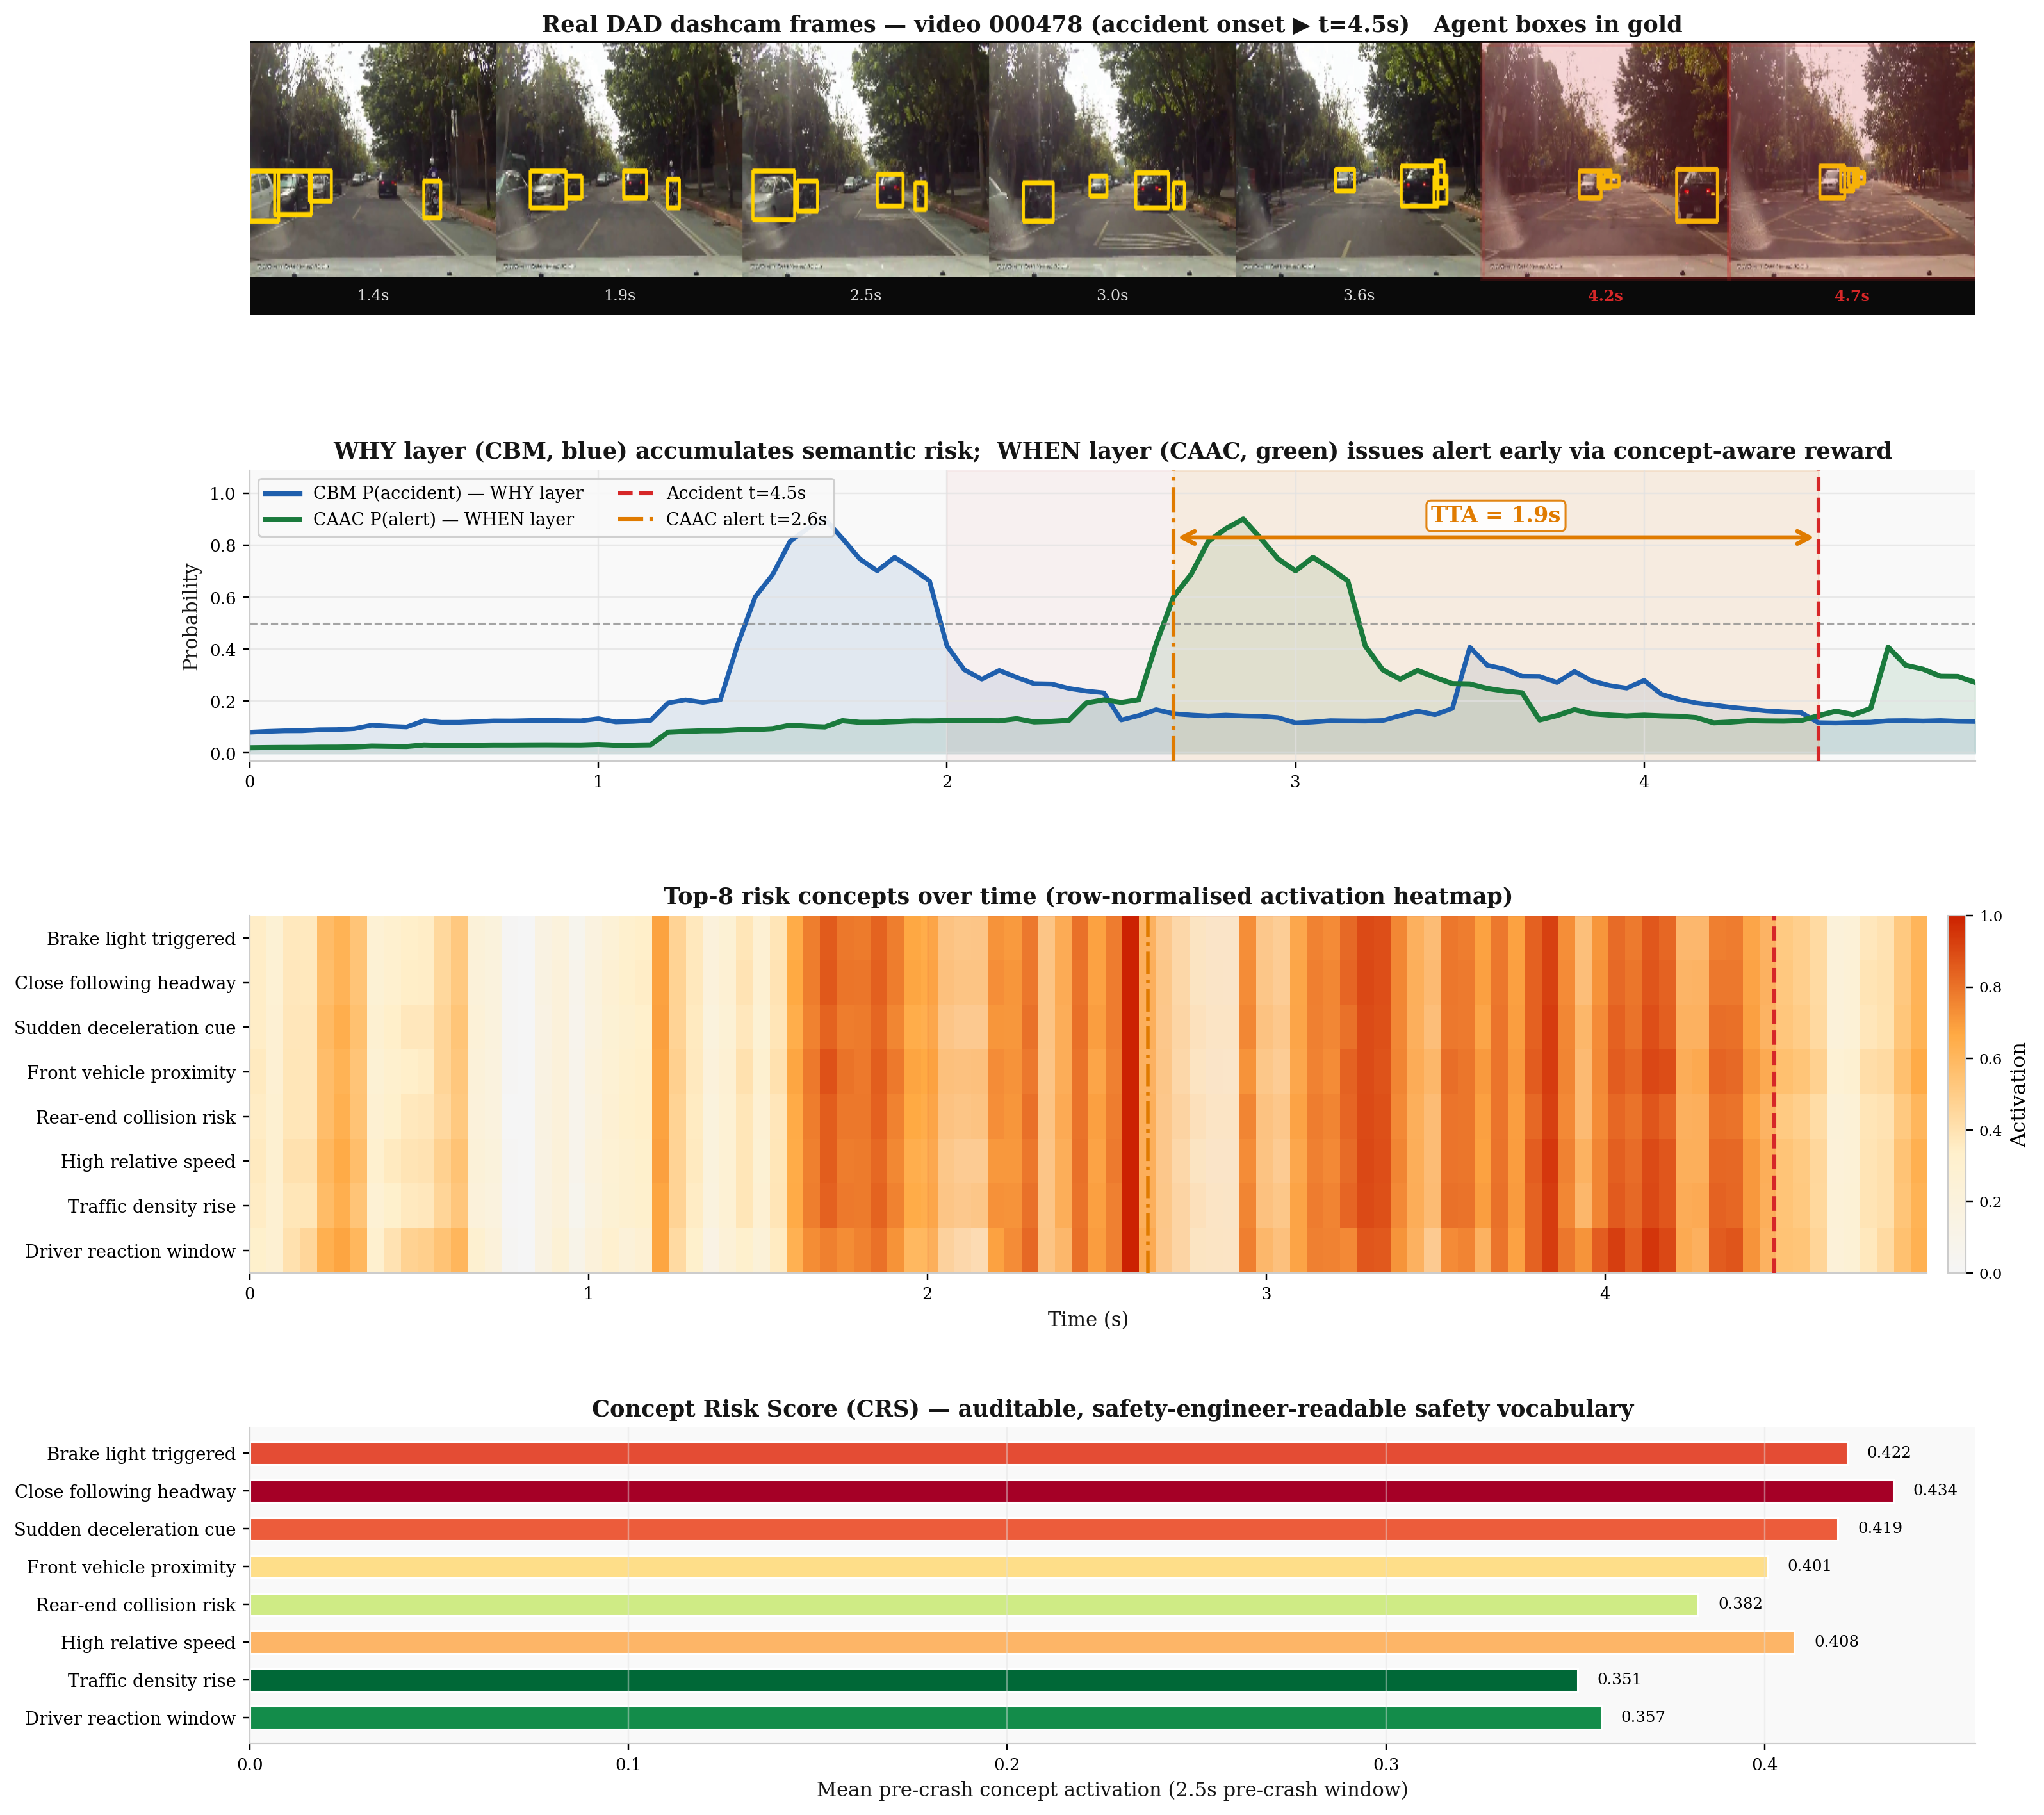
\includegraphics[width=0.98\textwidth]{../figures/insight_fig1_hero_dad_real.pdf}
  \caption{\textbf{A compact motivated example of the semantic interface.}
  One real crash sequence is read through named risk concepts before
  impact. The model does not expose only one final risk score; it exposes an
  inspectable semantic trajectory that can be inspected, compared, and audited
  as the scene evolves. The risk trajectory, concept activations, and alert
  marker are quantified in the headline, ontology, and timing-support evidence
  blocks rather than treated as a standalone case-study claim.}
  \label{fig:motivation}
\end{figure*}

\begin{figure*}[t]
  \centering
  \begin{subfigure}{0.495\textwidth}
    \centering
    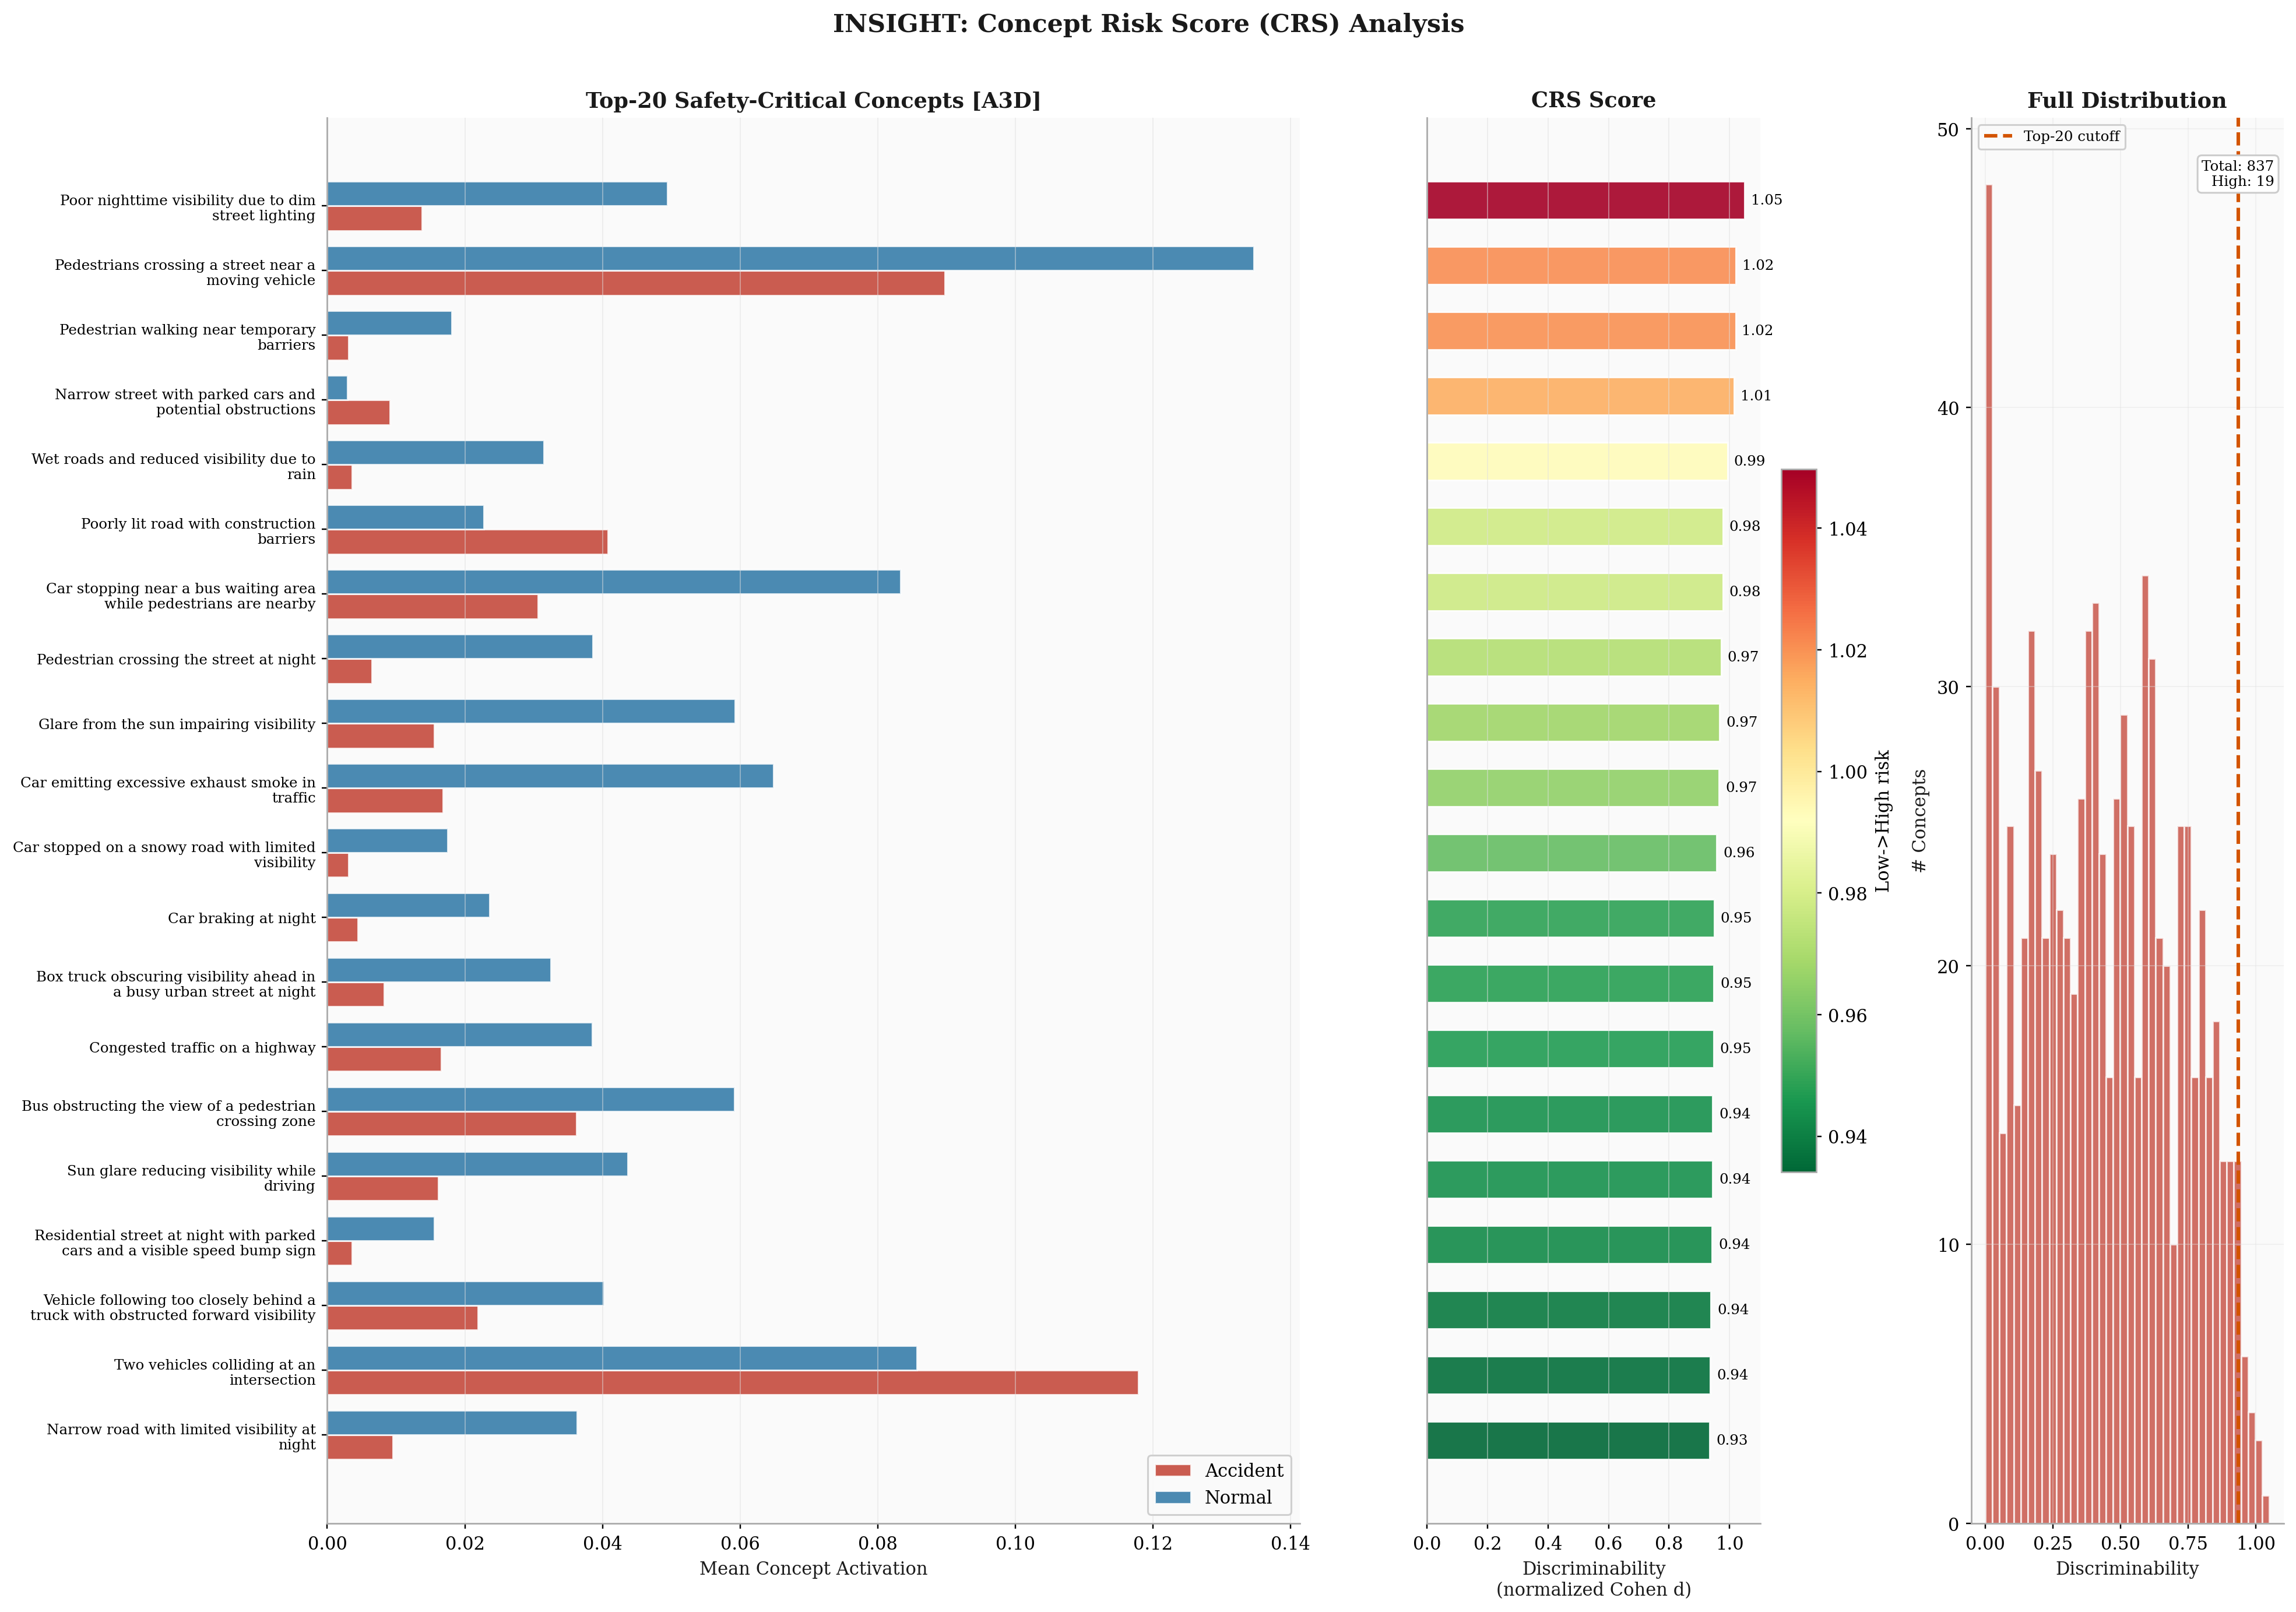
\includegraphics[width=\linewidth]{../figures/insight_fig3_crs_a3d.png}
    \caption{A3D CRS trace}
    \label{fig:vis_crs_a3d}
  \end{subfigure}
  \hfill
  \begin{subfigure}{0.495\textwidth}
    \centering
    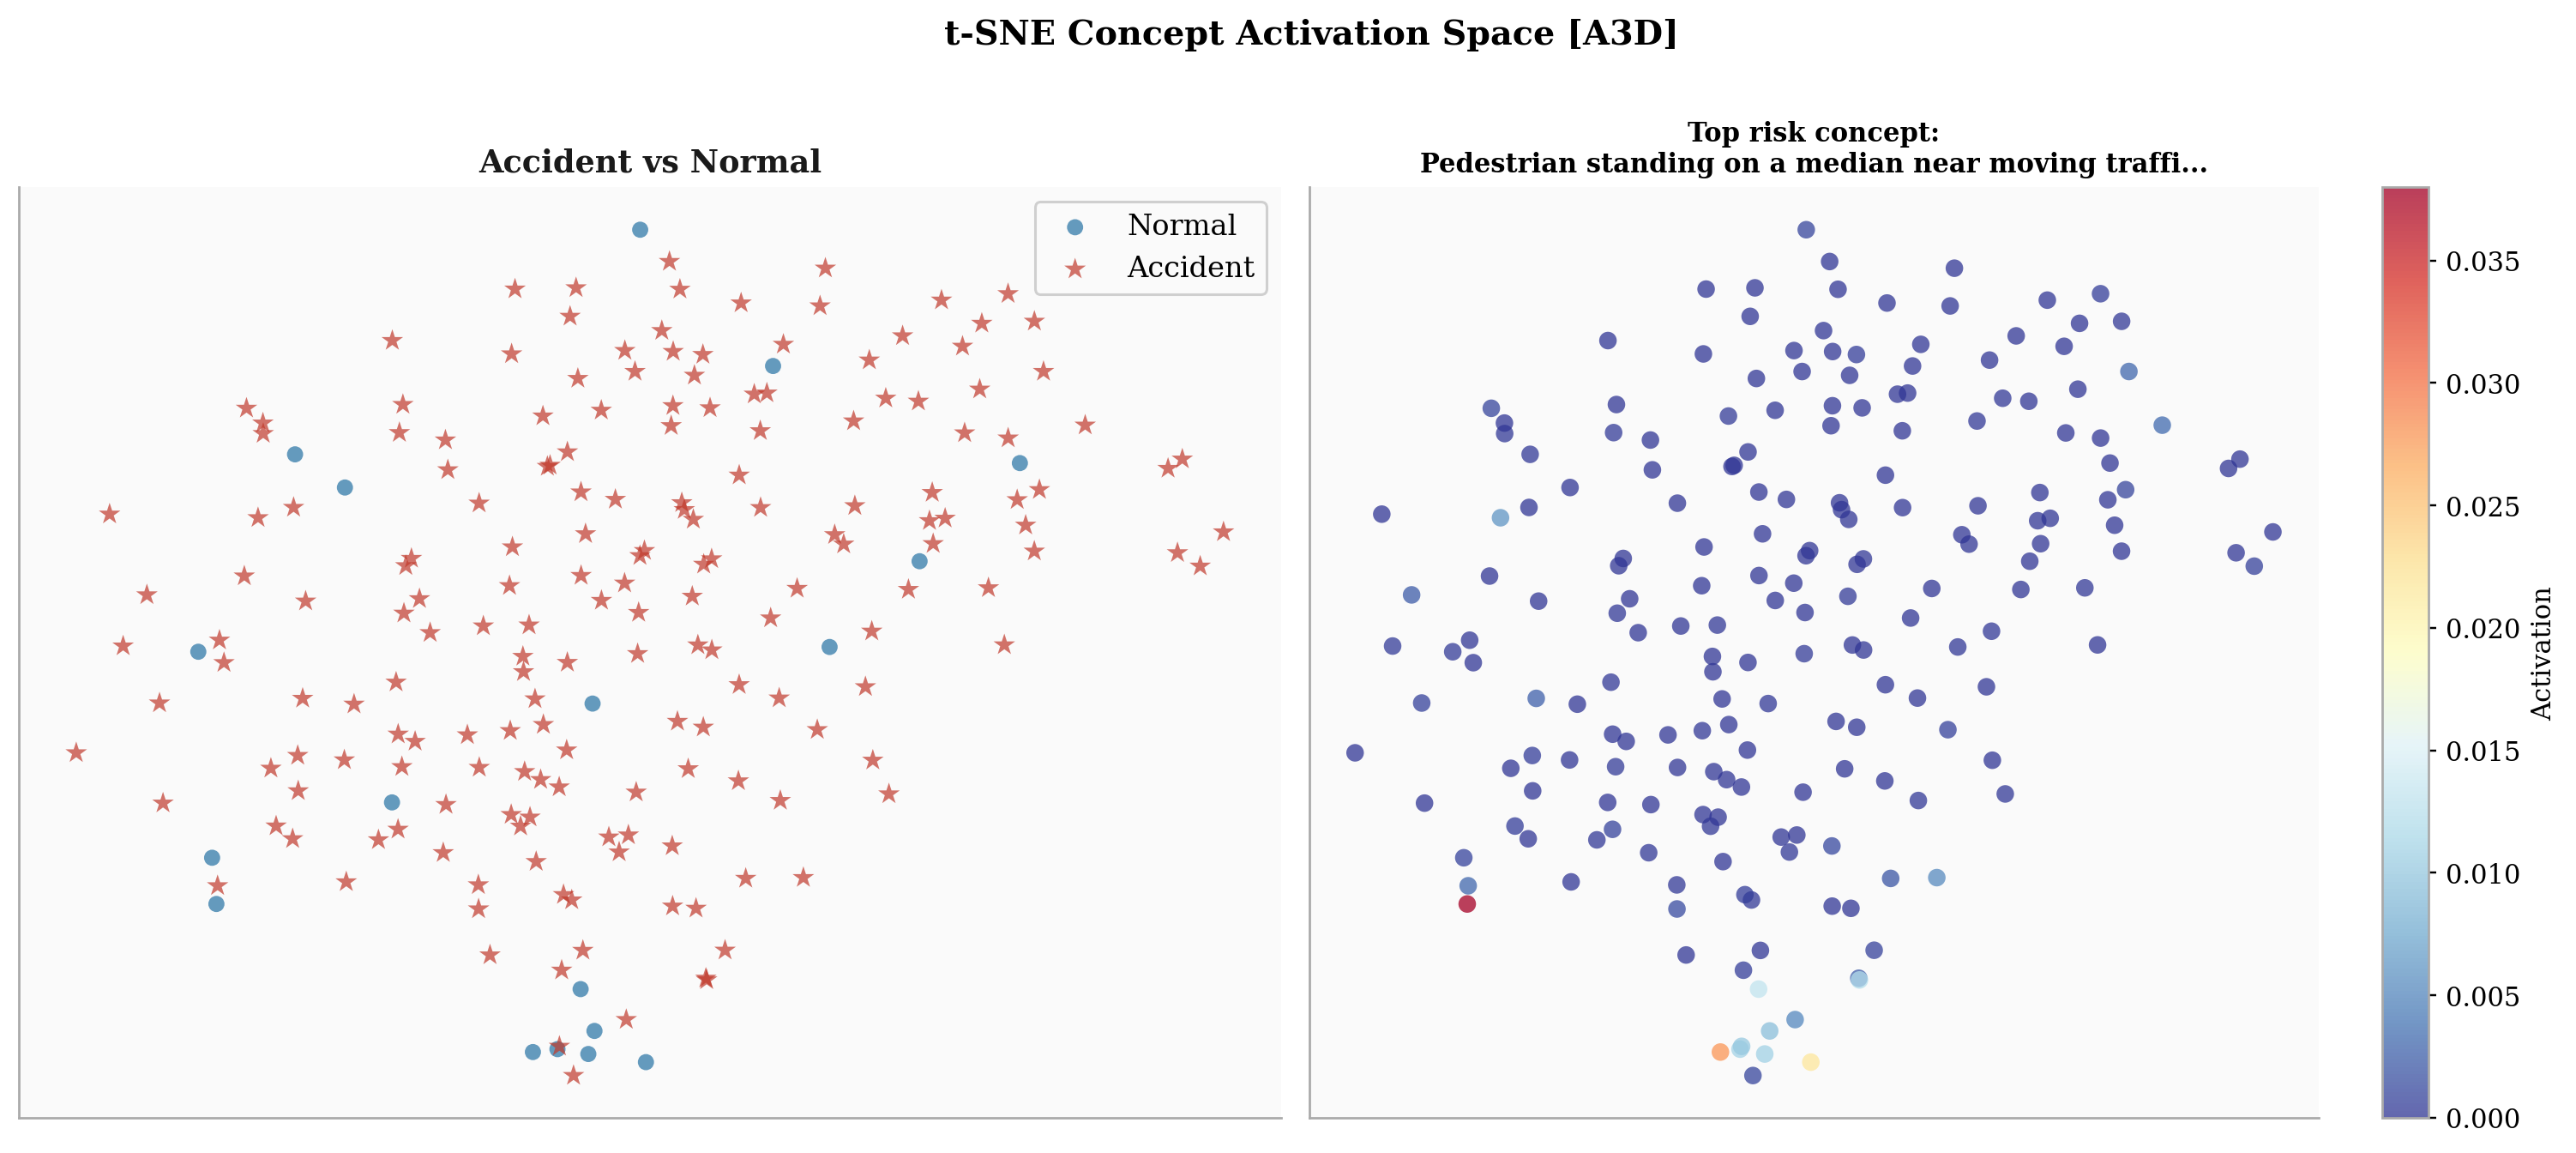
\includegraphics[width=\linewidth]{../figures/insight_fig4_tsne_a3d.png}
    \caption{A3D concept-space geometry}
    \label{fig:vis_tsne_a3d}
  \end{subfigure}
  \caption{\textbf{Interpretability bridge.}
  CRS and concept-space geometry provide a quick, intuition-first view of how the semantic interface behaves across pre-impact phases.
  }
  \label{fig:vis_bridge}
\end{figure*}

Figure~\ref{fig:motivation} and Figure~\ref{fig:vis_bridge} are intentionally paired with
Table~\ref{tab:a3d}, Table~\ref{tab:concept_sets}, and
Figure~\ref{fig:safety_utility}, Figure~\ref{fig:data_efficiency}, and
Figure~\ref{fig:intervention_gallery}:
the motivated example and bridge view show what the semantic interface looks like per case,
while the later headline/support blocks and the intervention gallery test whether
the same behavior survives quantitative, mechanistic, and cross-regime scrutiny.
The score trace and concept activations in Figure~\ref{fig:motivation} should
therefore be read as entry points to the quantitative ontology and timing
blocks, not as standalone evidence.


\paragraph{The missing object in accident anticipation: a semantic interface.}
The literature has made impressive progress on predictive quality.
Methods such as CRASH~\citep{liao2024crash}, CCAF-Net~\citep{liu2025ccaf}, and
LATTE~\citep{ZHANG2025103173} show that large-capacity models can deliver
strong AP and timing metrics. But from the perspective of interpretability and
scientific audit, a crucial object is still missing: an explicit semantic
interface between visual evidence and anticipation behavior. Without such an
interface, it is difficult to answer simple but important questions:
\emph{What risk concepts does the model actually rely on?}
\emph{How should those concepts be named, merged, or reviewed?}
\emph{Does changing the ontology change the predictive--timing trade-off?}

\paragraph{Why post-hoc explanation is not enough.}
Prior work offers only partial answers.
DRIVE~\citep{ref2} appends Grad-CAM after prediction;
W3AL~\citep{liao2024and} verbalizes accident location with an LLM;
other strong anticipation systems provide no intrinsic concept-level semantic
layer at all.
These approaches may help describe or localize a prediction, but they do not
turn the model's internal evidence into a stable, trainable, and auditable
representation that can be compared across runs or governed as a research
artifact. In a safety domain, that distinction matters: a system is easier to
audit and debug when its exposed semantics are part of the forward path, not an
after-the-fact visualization.

\paragraph{Scope we claim and do not claim.}
We make a focused claim: a language-grounded ontology is a governed research
variable, and that variable changes forecasting behavior in measurable ways under
matched training protocols.
We do not claim dataset-agnostic superiority, complete policy-level intervention control,
or that the same ontology choice is optimal across all driving distributions.
In this paper, CRASH materials are used as support-oriented stress and transfer
signals and are not pooled into the headline DAD/A3D claims.
This restraint is central to how we frame both our headline and support evidence.

\paragraph{Reading convention.}
We keep one compact convention throughout the paper: headline tables establish
the primary predictive position, controlled ontology comparisons test the
central semantic-interface claim, and stress analyses (including actor-policy
timing and CRASH transfer) are reported as bounded support evidence.

\paragraph{Our central insight.}
In accident anticipation, ontology construction should be treated as part of
the method rather than as hidden preprocessing.
A concept bottleneck is only as useful as the vocabulary it exposes. A generic
traffic word list is often too noisy; a fully manual ontology is hard to scale;
and an ungoverned pool of multimodal concept proposals is hard to defend as a
scientific interface. We therefore elevate concept construction itself to a
first-class modeling problem: sample risk-relevant frames, mine candidate risk
concepts, perform risk-first refinement, merge duplicates, balance semantic
families, and export a trainable ontology with explicit provenance. In the
language-interface framing of this paper, the key point is not merely that language is used
somewhere in the pipeline. It is that the language layer is governed:
canonical names, merge decisions, family structure, prompt policy, and light
review are all recorded as part of the research object.

\paragraph{\method{}: from risk ontology to trainable semantic interface.}
We propose \method{} (\textbf{In}terpretable \textbf{S}afety-\textbf{G}uided
accident anti\textbf{ci}pation via concep\textbf{t} bott\textbf{le}neck and
concept-aware actor-critic), but in this paper the center of gravity is
the \emph{language-grounded risk concept interface}. The model uses a
reproducible multimodal ontology pipeline to construct the semantic bottleneck,
then trains an interpretable anticipation system on top of that interface.
Concretely, the full framework contains
(i) a concept discovery and adjudication pipeline,
(ii) the \cbm{} semantic bottleneck,
(iii) the global \crs{} audit layer,
(iv)~\cgta{} for concept-linked temporal modeling,
(v)~\tsd{} for anticipatory representation learning, and
(vi) \caac{} as a downstream timing consumer of the concept state.
This design allows us to study not only model quality, but also how ontology
design changes the operating point of an interpretable anticipation system.
It also lets us separate three evidence questions cleanly: whether the
interface improves or preserves prediction quality, whether ontology choice
changes downstream behavior under matched training protocols, and whether the
release ontology's
canonical names and semantic families remain reviewable on the language side.

\paragraph{Contributions.}
\begin{itemize}[leftmargin=1.4em,topsep=2pt,itemsep=1pt]
  \item We argue that accident anticipation needs an auditable semantic interface, and that ontology construction should be treated as part of the method rather than hidden preprocessing.
  \item We introduce a reproducible multimodal risk-concept construction pipeline that mines, refines, merges, balances, and reviews risk concepts to produce a trainable ontology with explicit provenance, family structure, and canonical naming policy.
  \item We build \method{}, an interpretable anticipation framework that uses this ontology as a concept bottleneck and exposes auditable concept-level risk signals during prediction.
  \item We show, under matched training-protocol controls, that ontology choice changes the AP--mTTA operating point on both DAD and A3D, making the semantic interface itself an empirical variable rather than a cosmetic report.
  \item We pair predictive claims with language-side audits (500-frame pseudo-label and paraphrase stress), concept-level governance logs, and full review coverage for the released ontology. Under this protocol, \method{} reaches 93.40\% AP / 4.90s mTTA on A3D and 68.19\% AP on the canonical DAD line, while actor-policy timing is reported as scoped supporting evidence.
  \item We keep the central claim intentionally constrained: \method{} advances semantic-interface methodology and auditing, with the strongest current contribution in interpretability and controlled ontology science rather than policy-level causal intervention.
\end{itemize}

\section{Related Work}
\label{sec:related}

\paragraph{Accident anticipation and the benchmark tradition.}
Accident anticipation has moved from early temporal modeling for DAD~\citep{ref4} to larger multi-branch and graph-based predictors~\citep{ref45,ref17,ref32,ref36,ref37,ref208}. Large-capacity fusion systems now report strong AP and mTTA values on benchmark splits~\citep{liao2024crash,liu2025ccaf,ZHANG2025103173}, and several lines also add auxiliary interpretability signals~\citep{ref2,ref102}. The field therefore has a mature predictive toolbox, but most methods still optimize toward one central axis: score quality over time. In safety-critical forecasting, this leaves an unclosed question about what the model is using, and whether that ``why'' can be governed across runs and deployment settings.
The broader interpretability literature frames this same gap as one between local
faithfulness and reusable trust, with recent work emphasizing explicit interfaces
 explanations in risky settings~\citep{ribeiro2016loco,lundberg2017unified,doshi2017towards,rudin2019stop}. Some policy-oriented lines for safety timing introduce explicit uncertainty and control objectives~\citep{osband2016bootstrapped,konda1999actor}, yet they optimize decision behavior rather than providing a governed semantic vocabulary as an explicit method object.
In road-safety settings, deployment practice also raises this question to system
validity: interpretation is part of validation, not only visualization~\citep{who2023global,NHTSA2023}.
Related forecasting and trajectory work motivates the same concern about whether the
underlying representation is trustworthy under operational decisions~\citep{liao2024cognitive,ref13,ref23}.
The transportation literature further shows that operator safety judgment is tied to
semantic alignment and interpretable cueing, not solely raw confidence scores~\citep{kim2025understanding,guan2025experimental}.
Recent works on richer localization and accident context estimation~\citep{ref100,wang2024deepaccident} strengthen practical utility, while still leaving the semantic interface design itself mostly implicit.
Related datasets and precursor lines, including uncertainty-aware anticipation
and driver-attention-oriented benchmarks~\citep{ref1,ref33,fang2021dada,karim2023attention},
similarly emphasize predictive behavior more than governed semantic interfaces.

\paragraph{Governance and human factors context.}
Recent safety standards and practitioner guidance stress that model evidence is one part of readiness.
Validation protocols for safety-critical forecasting increasingly require interpretable
artifacts, explicit uncertainty behavior, and auditability paths, especially when
warnings trigger human or automation actions~\citep{who2023global,NHTSA2023}.
\method{} positions the semantic interface as one such artifact: a method-level
object whose names, families, and timing behavior are reviewable across protocol
choices.

In high-stakes settings, this matters because interpretability without governance
is often non-actionable. Concept-level claims require evidence about how concepts are
constructed, maintained, and constrained across runs; the paper therefore treats the
ontology and scoring pipeline as part of the model method and not as a detached
annotation step. This aligns with the broader call in high-stakes ML to keep
modeling choices auditable by design rather than evaluated only after training
~\citep{doshi2017towards,rudin2019stop}.

\paragraph{Post-hoc explanation versus embedded semantics.}
Post-hoc methods such as feature attribution and verbalization provide useful
diagnostics (e.g., LIME and SHAP) but are often attached after prediction.
DRIVE adds attention
visualizations to the output path~\citep{ref2}; W3AL introduces natural language
reporting around location and timing~\citep{liao2024and}. These designs increase
transparency to users but do not usually enforce a stable semantic state that is
shared by training, evaluation, and intervention. In our setting, this distinction is
critical: an attached explanation can show what looked important for one
prediction, while an embedded semantic interface must support reusable claims
about what risk concepts are consistently represented by the model.
\method{} positions itself in this gap by making the concept state part of the
model's forward computation.

\paragraph{Interpretability and concept-level learning.}
Concept bottlenecks provide a principled intermediate layer that remains
human-interpretable and mathematically tractable~\citep{tishby2000information,koh2020concept}.  
Subsequent work has reduced reliance on dense annotations and expanded
concept-supervision design~\citep{zarlenga2022concept,yuksekgonul2023posthoc,oikarinen2023label}.  
In accident anticipation, those ideas are harder to apply because concepts must
be temporally meaningful and task-governable across long horizons. This is why
our method treats concept vocabulary construction as a first-class component,
not a fixed side input.

This framing also distinguishes \method{} from post-hoc explanation pipelines.
In the broader accident-anticipation literature, most prior work does not treat
concept vocabulary as a tunable, auditable method component, so semantic signals
cannot be directly governed across matched launches.
Attribution methods such as Grad-CAM
\citep{selvaraju2017gradcam} explain individual predictions, while
concept-activation techniques such as TCAV
\citep{kim2018tcav} test global class-level concept sensitivity.
Both are useful, but neither becomes a reusable interface artifact unless the
concept layer is constructed, constrained, and audited as part of the model.
This also makes the actor-policy caution more central: prior reinforcement-learning
and credit-assignment work emphasize that policy- or intervention-level claims require explicit control-focused validation, not prediction-only benchmarking~\citep{konda1999actor,meulemans2023cocoa}.
Our contribution is therefore not only semantic readability, but the governance
of that interface under matched launchers and matched family-level controls.
Automatic concept discovery lines such as ACE~\citep{ghorbani2019ace} are also
relevant here: they motivate scalable concept proposal, but our focus is the
downstream governance and deployment of a fixed, auditable concept interface.

\paragraph{Language-grounded ontology for multimodal safety systems.}
Recent progress in vision-language pretraining enables language to act as
semantic glue for risky-scene understanding~\citep{radford2021learning,jia2021align}.  
In driving, VL supervision has improved scene grounding and text-aware
reasoning~\citep{liao2024gpt,shi2025scvlm}. In contrast to trajectory-prediction systems that rely heavily on map constraints and route semantics~\citep{ref215}, we use it as a conservative
bootstrap: CLIP-style pseudo-labeling and paraphrase stress tests produce
candidate semantic structure while avoiding claims of full semantic correctness.
Temporal distillation then anchors the interface to future-aware representations,
so the semantic layer is coupled to anticipation timing~\citep{fang2022traffic}.

\paragraph{Ontology governance as method, not ornament.}
Compared with systems where semantic terms are implicit prompts, prompt templates,
or uncontrolled phrase pools, our pipeline explicitly performs mining,
canonicalization, family balancing, and light review. This changes the research
question from \emph{``Can we predict with higher AP?''} to \emph{``How does
semantic design change behavior under matched training and evaluation?''}.  
That shift aligns with current language-oriented evaluation culture because the
interface itself is now an accountable artifact: its names, merges, and coverage can
be inspected and compared.

\paragraph{Position in this paper.}
Our paper is not attempting to turn accident anticipation into a text-generation
task. Instead, it studies whether a governed, language-grounded interface can be
designed for a forecasting pipeline, and whether that interface changes what can
be audited and compared. In this framing, \method{} contributes primarily at the
representation-design layer: a reproducible ontology construction path and a
matched-evaluation protocol that turns ontology choice into an explicit variable.
\method{} is strongest where this differs from prior accident systems: it links
concept construction, model training, and intervention-oriented auditing into one
methodological unit rather than treating semantics as a visualization overlay.

\section{\method: A Language-Grounded Semantic Interface for Accident Anticipation}
\label{sec:method}

We present \method{}, a framework whose central object is a
\emph{language-grounded risk concept interface}. The interface is built first
through a reproducible ontology pipeline and then used as the semantic
bottleneck of an interpretable anticipation model. Figure~\ref{fig:framework}
summarizes the full system.
This design follows the information-bottleneck principle in that a constrained,
named intermediate space is explicitly optimized for downstream utility while
remaining inspectable to users and protocol designers~\citep{tishby2000information}.

\begin{figure*}[t]
  \centering
  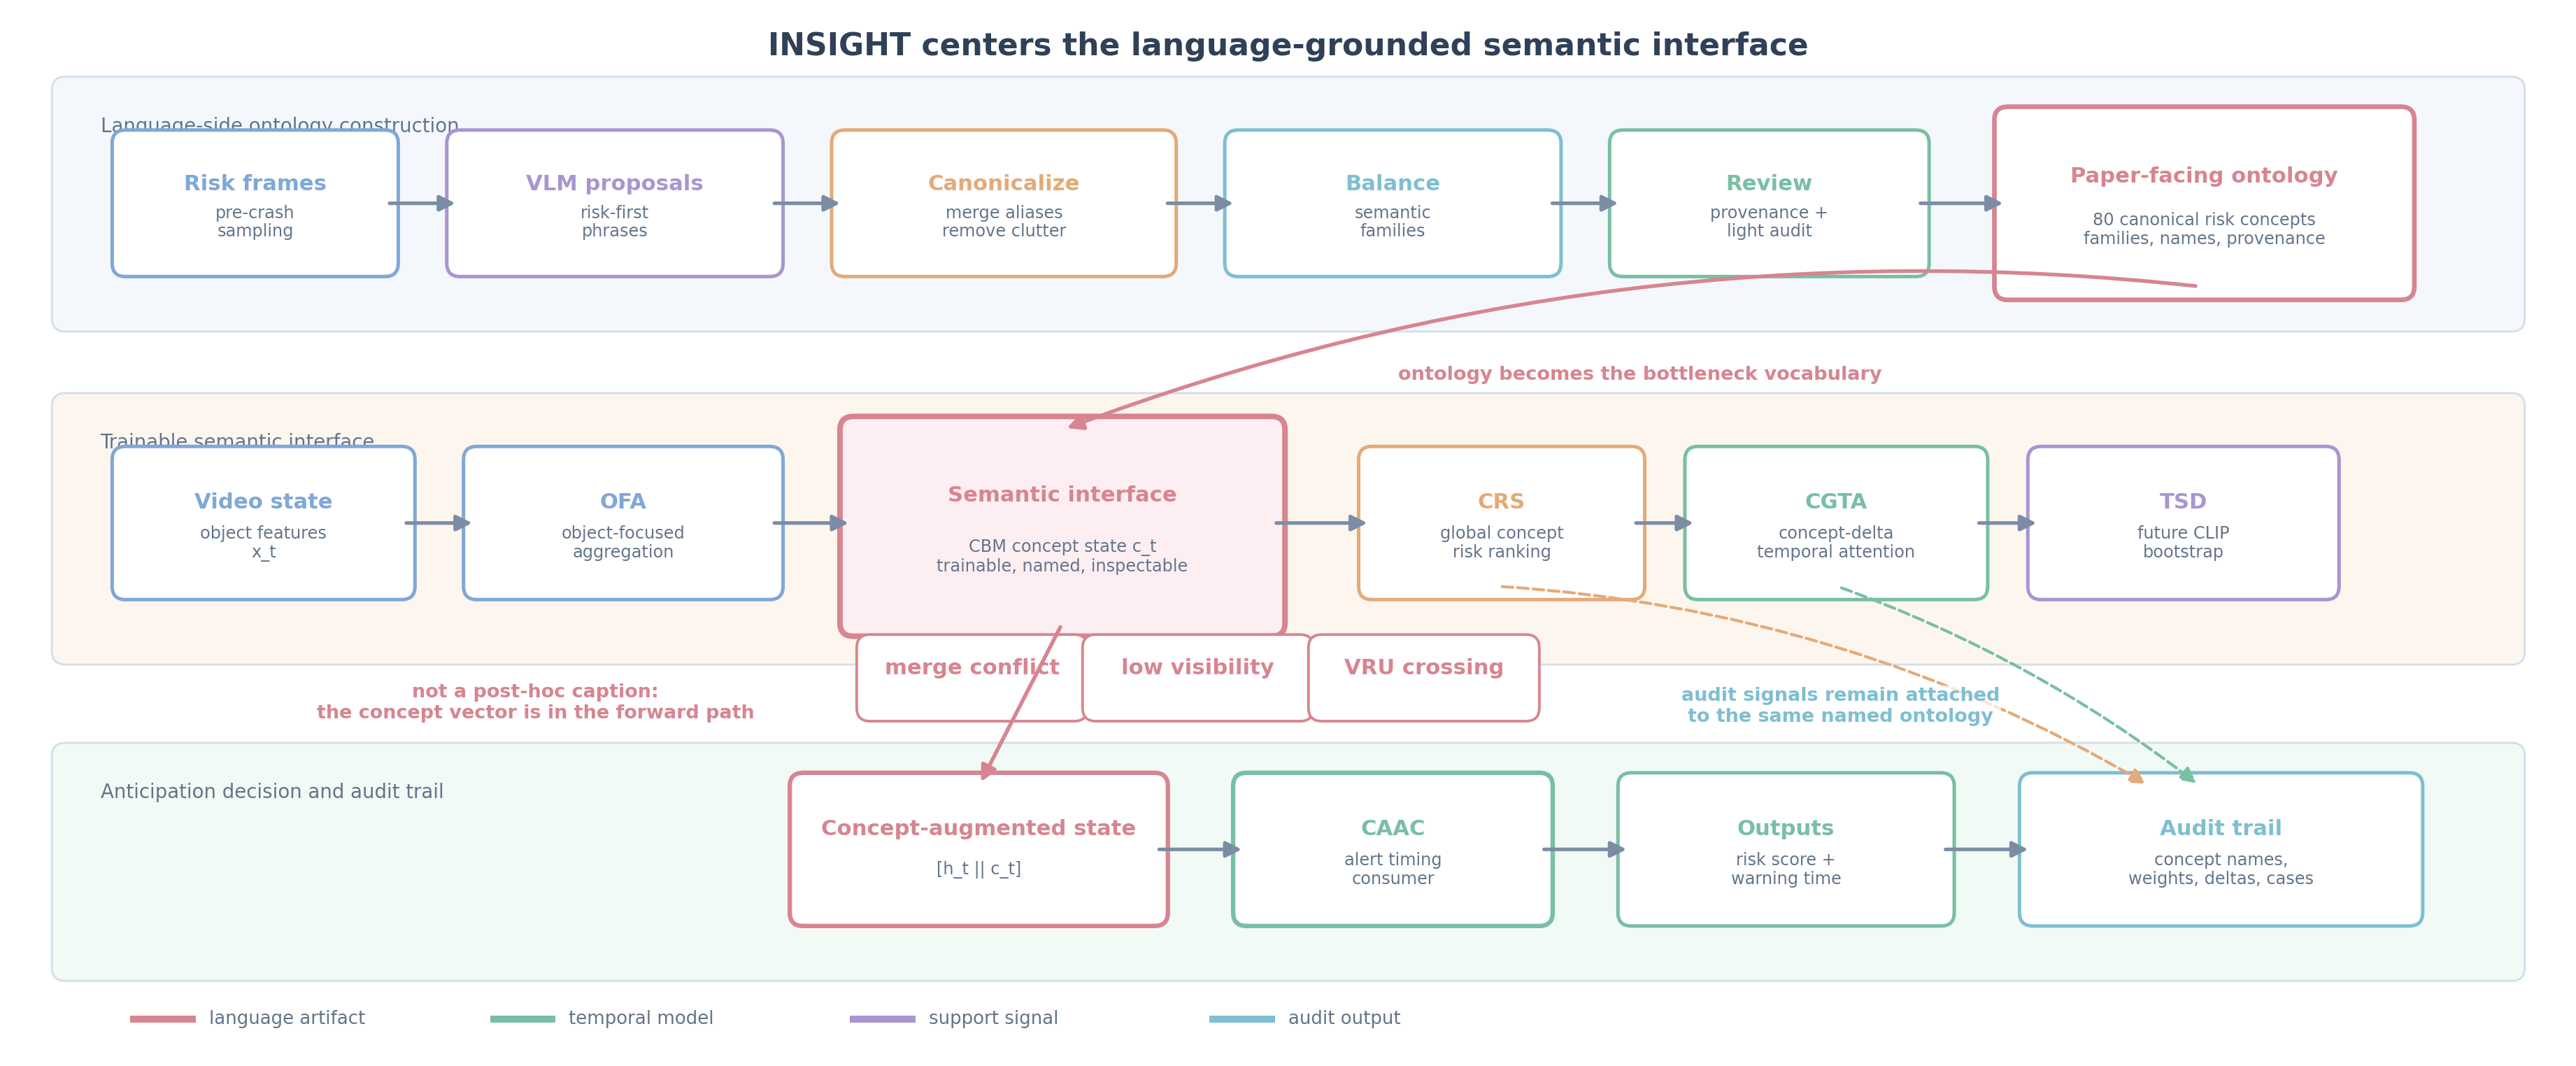
\includegraphics[width=\textwidth]{../figures/insight_framework.pdf}
  \caption{\textbf{\method{} as a semantic-interface pipeline.}
  Per-frame object features are aggregated, mapped into an explicit concept
  space, and then consumed by downstream anticipation modules. In this paper,
  the most important object is the semantic interface:
  the ontology construction pipeline produces the concepts, the CBM exposes
  them as trainable state, CRS and CGTA make them auditable over time, and the
  timing module consumes them as part of its decision state.}
  \label{fig:framework}
\end{figure*}

\subsection{Problem Setup and Design Scope}

Given a dashcam video $\{\mathbf{x}_t\}_{t=1}^T$ with
$\mathbf{x}_t \in \mathbb{R}^{N \times D}$, a binary label
$y \in \{0,1\}$, and time-of-accident $\tau$, accident anticipation is usually
framed as predicting whether an accident will occur from a video prefix. Our
goal is more specific: to expose a semantic interface that allows the model's
risk evidence to be named, compared, and audited while retaining competitive
predictive behavior.

We use the following idealized objective as a motivating target:
\begin{equation}
  \max_{\theta}\; \mathbb{E}[\mathrm{TTA}]
  \quad \text{s.t.} \quad \mathrm{AP}(\theta) \geq \mathrm{AP}_{\text{base}},
  \label{eq:objective}
\end{equation}
where TTA is the warning lead time and AP is the standard precision--recall
metric. This equation simply states the target operating regime: improve lead
time without sacrificing predictive quality. Our methodological contribution is
the semantic interface that lets us study how ontology design changes this
operating point.

\subsection{Ontology Construction as Method}

\paragraph{Why ontology construction belongs in the method section.}
A concept bottleneck is only as useful as the concept vocabulary it exposes.
In accident anticipation, a generic traffic lexicon is often too broad, while
a fully manual ontology is difficult to scale and hard to govern
systematically. We therefore treat ontology construction as part of the method
rather than as hidden preprocessing. The aim is to produce \emph{trainable,
auditable, and comparable} risk primitives rather than a loose list of scene
descriptions.

\paragraph{Stage 1: risk-oriented frame mining.}
We first sample pre-crash frames from positive videos to cover diverse traffic
geometries, actor interactions, visibility conditions, and accident precursor
patterns. Sampling is intentionally risk-oriented: the goal is to expose
emerging hazards rather than to maximize generic visual diversity. This reduces
annotation cost while preserving the semantic support needed for downstream
concept discovery.

\paragraph{Stage 2: multimodal risk concept proposal.}
Given the sampled frames, a multimodal model proposes candidate concepts,
risk factors, and coarse semantic families. Our prompts ask explicitly for
\emph{risk-first} concepts, such as cut-in behavior, closing distance,
visibility degradation, or vulnerable-road-user interaction, instead of generic
scene captions. The output of this stage is a noisy but high-recall pool of
candidate accident precursors.

\paragraph{Stage 3: risk-first refinement and canonical merge.}
The raw candidate pool is then refined into reusable risk primitives. We
prioritize risk-relevant or precursor-like factors, remove obvious
background clutter, merge near-duplicates, and normalize phrasing toward short
canonical names. This step is not merely cosmetic. Stable downstream training
benefits more from reusable concepts than from many near-synonymous
micro-labels, so the refinement policy intentionally favors semantic stability
over maximal lexical granularity.

\paragraph{Stage 4: family balancing and light human review.}
The ontology is further polished through family-level coverage auditing,
duplicate-cluster consolidation, and a light human review pass. The result is a
\emph{paper-facing semantic interface}: compact enough to present clearly, rich
enough to retain major accident precursor families, and explicit enough to
support provenance tracking, case studies, and matched ontology comparisons.

\paragraph{Stage 5: export as a trainable research asset.}
The final ontology is stored with canonical concept names, family metadata,
merge provenance, and review notes. This matters because the ontology is not
used only for figures. It is encoded and deployed as the actual bottleneck
vocabulary of the model, so ontology construction is evaluated not just by
semantic plausibility but by whether the resulting interface survives contact
with downstream learning.

\paragraph{What makes the interface language-grounded and governed.}
The paper's claim does not rest on any single multimodal model being perfectly
right about frame semantics. It rests on a governed language layer: prompts are
risk-oriented, outputs are canonicalized into short stable names, semantic
families are balanced explicitly, and retained concepts carry provenance and
review metadata. This matters because the scientific question is not only
whether concepts can be proposed, but whether the resulting ontology is stable
enough to function as a named interface between visual evidence and downstream
anticipation behavior.

\begin{figure*}[t]
  \centering
  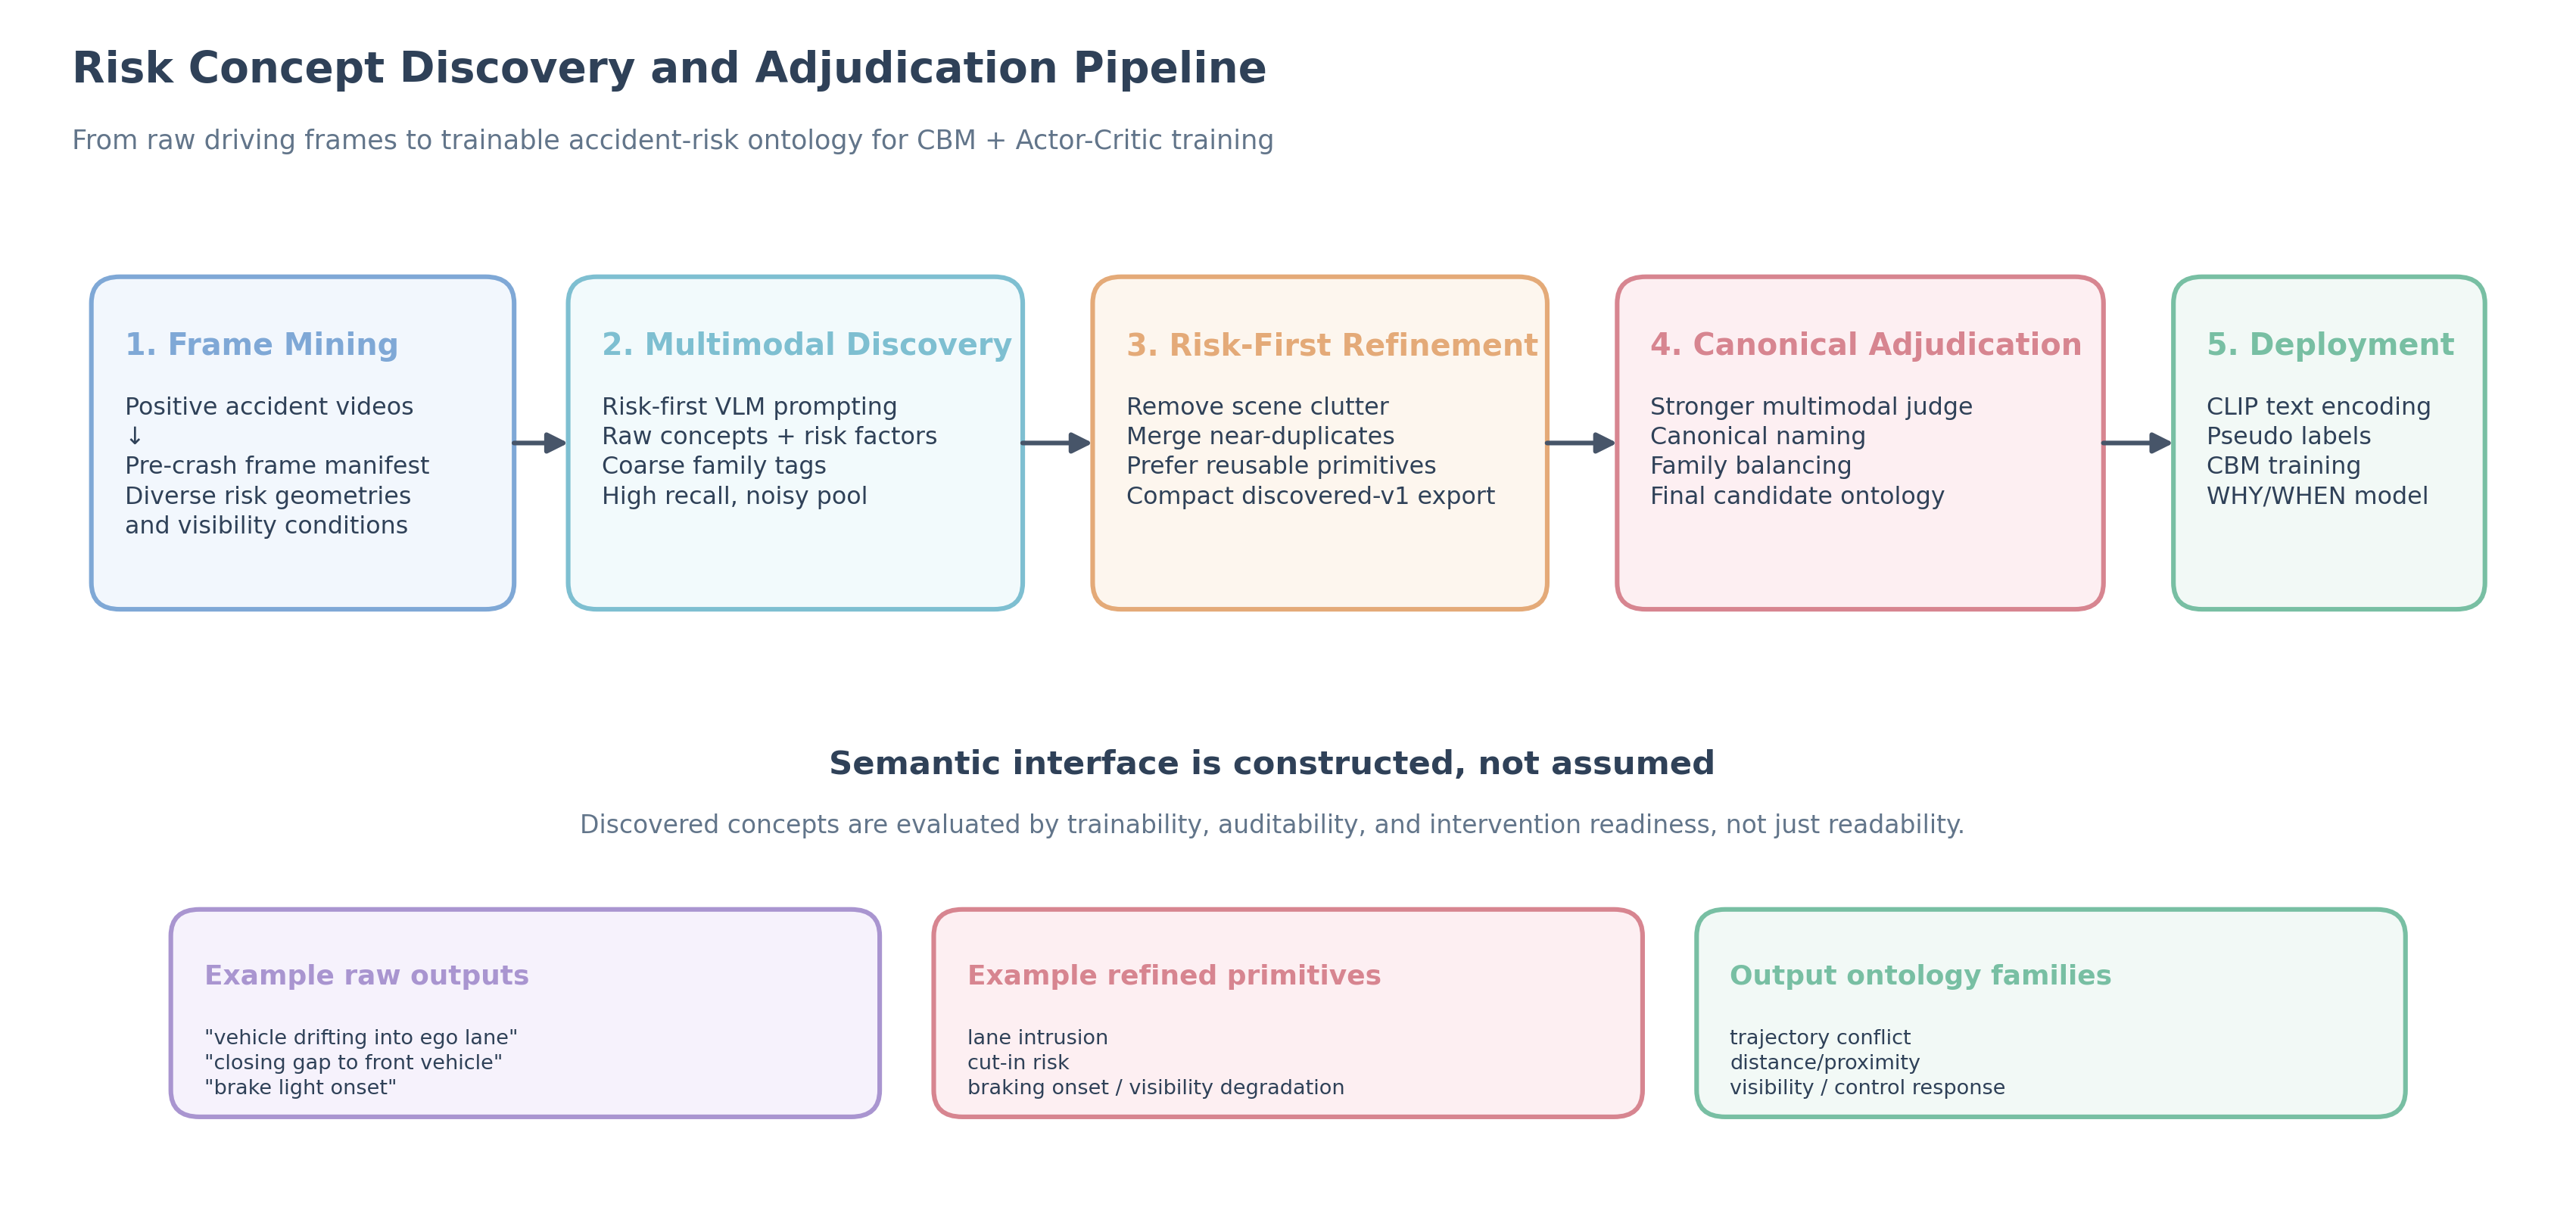
\includegraphics[width=0.98\textwidth]{../figures/insight_fig_concept_pipeline.pdf}
  \caption{\textbf{End-to-end risk ontology construction.}
  Starting from sampled pre-crash frames, the pipeline performs multimodal
  concept proposal, risk-first refinement, duplicate consolidation, family
  balancing, and light human review to produce a trainable ontology for the
  concept bottleneck. The ontology is therefore a reproducible methodological
  component rather than a hidden vocabulary assumption.}
  \label{fig:concept_pipeline}
\end{figure*}

\subsection{Model Overview}

Once the ontology is fixed for a run, \method{} uses it as the semantic
bottleneck of the anticipation model. The per-frame forward pass is
\begin{align*}
  \mathbf{x}_t
  &\xrightarrow{\text{OFA}} \mathbf{o}_t
  \xrightarrow{\cbm} (\mathbf{c}_t,\mathbf{e}_t)
  \xrightarrow{\crs} \rho_t \\
  &\xrightarrow{\cgta} \mathbf{g}_t
  \xrightarrow{\text{GRU}} \mathbf{h}_t
  \xrightarrow{\caac} (p_t, a_t, V_t).
\end{align*}
The key design choice is that downstream anticipation does not consume only an
opaque hidden state. It also consumes the explicit concept activations
$\mathbf{c}_t$, which makes the system's semantic interface available to both
prediction and timing.

\subsection{Object-Focused Aggregation}

Each frame contains $N$ object features. We aggregate them through
Object-Focused Attention (OFA):
\begin{align}
  \alpha^n_t &= \mathrm{softmax}_n\bigl(\mathbf{w}_a^\top
    \tanh(\mathbf{W}_o \mathbf{x}^n_t)\bigr), \\
  \mathbf{o}_t &= \sum_{n=1}^N \alpha^n_t\,\mathbf{W}_f \mathbf{x}^n_t.
\end{align}
This provides a compact frame representation that preserves actor-level
salience before the semantic bottleneck is applied.

\subsection{Concept Bottleneck Module}

The Concept Bottleneck Module maps the aggregated frame representation to
$K$ interpretable risk concepts, where $K$ depends on the ontology used in the
run ($K{=}837$ for the historical full set and smaller values for compact
ontologies):
\begin{align}
  \mathbf{c}_t &= \sigma(\mathbf{W}_c \mathbf{o}_t + \mathbf{b}_c)
    \in [0,1]^K, \\
  \mathbf{e}_t &= \mathrm{LayerNorm}(\mathbf{W}_d \mathbf{c}_t + \mathbf{b}_d).
\end{align}
The vector $\mathbf{c}_t$ is the paper's strongest interpretability object:
each dimension corresponds to a named risk concept in the ontology.

\paragraph{Pseudo-label supervision.}
We supervise the bottleneck with CLIP-derived pseudo-labels
$\hat{\mathbf{c}}_t \in \{0,1\}^K$. For each frame, a concept is marked
positive if its similarity score lies in the frame-wise top-$m$ set
($m{=}3$ in the main recipe). The auxiliary loss is
\begin{equation}
  \mathcal{L}_{\text{aux}}
  = \frac{1}{K}\,\mathrm{BCE}(\mathbf{c}_t,\,\hat{\mathbf{c}}_t).
\end{equation}
We interpret these pseudo-labels as a semantic bootstrap rather than as a claim
of perfect concept correctness.

\subsection{Concept Risk Score and Temporal Semantic Modeling}

\paragraph{Concept Risk Score (CRS).}
To expose a global audit signal, we learn per-concept risk weights
$\mathbf{w}_{\text{risk}} \in \mathbb{R}^K$ and compute
\begin{equation}
  \rho_t = \sigma(\mathbf{w}_{\text{risk}})^\top \mathbf{c}_t.
  \label{eq:crs}
\end{equation}
Unlike attention weights that vary from case to case, CRS provides a global
ranking that can be inspected as part of the semantic interface. In the current
paper, however, we treat CRS as an audit-oriented support signal rather than as
a fully mature standalone product claim.

\paragraph{Concept-Guided Temporal Attention (CGTA).}
Standard temporal attention is often difficult to interpret. We instead drive
temporal attention with concept deltas so that changes in semantic state guide
where the model looks in history:
\begin{align}
  \Delta\mathbf{c}_t &= \mathbf{c}_t - \mathbf{c}_{t-1}, \\
  \alpha_{t,s} &=
    \frac{\exp\bigl((\mathbf{W}_Q\Delta\mathbf{c}_t)^\top
      (\mathbf{W}_K\mathbf{h}_s)/\sqrt{h}\bigr)}
    {\sum_{s'=1}^{t-1}\exp\bigl((\mathbf{W}_Q\Delta\mathbf{c}_t)^\top
      (\mathbf{W}_K\mathbf{h}_{s'})/\sqrt{h}\bigr)}, \\
  \mathbf{g}_t &= \lambda_{\text{gate}}\sum_{s=1}^{t-1}\alpha_{t,s}\mathbf{W}_V\mathbf{h}_s
    + (1-\lambda_{\text{gate}})\mathbf{h}_{t-1}.
\end{align}
When a risk concept spikes, CGTA highlights the historical frames that likely
caused the change, creating a temporal audit trail for the semantic layer.

\subsection{Temporally Shifted Distillation}

To inject anticipatory information into the hidden representation, we distill
future CLIP features into the current state:
\begin{equation}
  \mathcal{L}_{\text{TSD}}
  = \bigl\|\mathbf{W}_{\text{TSD}}\mathbf{o}_t
    - \mathrm{sg}(\mathbf{f}^{\text{CLIP}}_{t+\delta})\bigr\|_2^2,
  \label{eq:tsd}
\end{equation}
where $\delta{=}5$ frames and $\mathrm{sg}(\cdot)$ denotes stop-gradient.
TSD is a support module: it encourages the model to encode where the scene is
headed, while the paper's main scientific focus remains the semantic interface
that drives downstream anticipation.

\subsection{Concept-Conditioned Timing Module}

\paragraph{Why timing still matters in this paper.}
Although this paper centers the semantic interface, accident
anticipation remains a temporal decision problem. The role of the timing module
is therefore to consume the concept state and expose how semantic evidence
shapes warning behavior. In the experiments, semantic-layer and ontology
comparisons carry the central claim, while actor-policy timing is reported as a
downstream transfer test of that interface.

\paragraph{State.}
The timing module consumes a concept-conditioned state
\begin{equation}
  \mathbf{s}_t = [\mathbf{h}_t \| \mathbf{c}_t].
  \label{eq:state}
\end{equation}
Architecturally, this is the crucial link from language-grounded concepts to
downstream temporal behavior: the timing module no longer acts on an opaque
latent vector alone.

\paragraph{Actor and Critic.}
The actor-critic formulation follows a standard policy-optimization setup
\citep{konda1999actor,sutton2018reinforcement}.
We parameterize an actor and critic over the concept-conditioned state:
\begin{align}
  \pi(a_t \mid \mathbf{s}_t)
    &= \mathrm{Softmax}(\mathbf{W}_\pi \mathbf{s}_t + \mathbf{b}_\pi), \\
  V(\mathbf{s}_t)
    &= \mathbf{w}_V^\top \tanh(\mathbf{W}_{V_1}\mathbf{s}_t).
\end{align}

\paragraph{Reward.}
Each video is a finite-horizon episode. The reward favors early correct alerts
and penalizes false alarms and misses:
\begin{equation}
  \mathfrak{r}_t = \begin{cases}
    \begin{aligned}[t]
      \lambda_r \cdot \dfrac{\tau - t}{\tau}\\
      \cdot (1 + \beta\, b_t)
    \end{aligned}
      & \text{first positive alert, } t < \tau \\[4pt]
    -\lambda_p & \text{false alert or miss} \\[4pt]
    +\varepsilon & \text{wait before end}
  \end{cases}
  \label{eq:reward}
\end{equation}
where $b_t = \sigma(\mathbf{w}_b^\top \mathbf{c}_t)$ is a learnable concept
bonus. This term encourages the policy to favor early alerts that are backed by
strong concept evidence.

\paragraph{Actor-Critic objective and evaluation scope.}
With advantage $A_t = R_t - V(\mathbf{s}_t)$ and discounted return $R_t$, the
Actor-Critic loss is
\begin{align}
  \mathcal{L}_{\text{AC}}
  &= -\mathbb{E}_t[\log\pi(a_t\mid\mathbf{s}_t)\,A_t] \nonumber\\
  &\quad + \lambda_V \mathbb{E}_t[(V(\mathbf{s}_t)-R_t)^2] \nonumber\\
  &\quad - \lambda_H \mathcal{H}[\pi(\cdot\mid\mathbf{s}_t)].
  \label{eq:ac_loss}
\end{align}
In the current paper, the canonical headline AP/mTTA numbers are still derived
from the classifier trajectory rather than from a fully validated standalone
actor policy. We therefore use CAAC to test how much timing behavior transfers
to a concept-conditioned policy, while keeping the canonical predictive
headline on the classifier branch and avoiding stronger policy-level claims than
the current evidence supports.

\subsection{Total Training Objective}

The overall objective balances classification, concept supervision, timing
training, and anticipatory distillation:
\begin{equation}
  \mathcal{L}
  = \mathcal{L}_{\text{CE}}
  + \lambda_{\text{aux}}\,\mathcal{L}_{\text{aux}}
  + \lambda_{\text{AC}}\,\mathcal{L}_{\text{AC}}
  + \lambda_{\text{TSD}}\,\mathcal{L}_{\text{TSD}}.
  \label{eq:total_loss}
\end{equation}
We use a warmup-and-ramp schedule so that concept learning stabilizes before
the timing objective becomes dominant. This matters because the timing module
is only useful if the semantic state it consumes is already coherent.

\subsection{Design Rationale and Complexity Notes}
\label{sec:theory}

\paragraph{Complexity.}
The dominant costs come from the recurrent backbone and the concept-dependent
projections. With the current hidden sizes and ontology sizes, these costs
remain compatible with a 30M-parameter model. The practical point is modest but
important: exposing a semantic interface does not require the very large model
scale used by several recent non-interpretable anticipation systems.

\paragraph{Why intervention is structurally meaningful.}
If a concept edit $\Delta\mathbf{c}$ is applied before prediction, the timing
state becomes $\mathbf{s}'_t = [\mathbf{h}_t \| \mathbf{c}_t + \Delta\mathbf{c}]$.
This does not prove that every trained model will respond monotonically to
every edit. What it does show is that concept edits act on the same state
consumed by downstream timing. For this reason, the intervention studies in the
experiments section are meaningful as tests of a \emph{structurally
intervenable} interface, even though full policy-level causal validation lies
beyond the scope of the current paper.

\section{Experiments}
\label{sec:experiments}

\subsection{Experimental Setup}

\paragraph{Datasets.}
\textbf{DAD}~\citep{ref4}: 1,750 dashcam videos (620 accident,
1,130 non-accident) from six Taiwanese cities, split 1,280/450
train/test. Videos are 5\,s at 20\,fps (100 frames).
\textbf{A3D}~\citep{liao2024crash}: 1,199 videos (960/239) at 10\,fps,
100 frames, spanning diverse East Asian urban accident types.
\textbf{Coverage design.}
We choose two datasets with complementary hazard dynamics rather than building
an oversized benchmark zoo: DAD stresses short-horizon, high-noise transitions,
while A3D tests whether a semantic interface can expose earlier, progressive
precursors at cleaner operating points.
To add an additional evidence dimension, we also run data-efficiency probes on
CRASH with the same recipe family and report the resulting curve in a dedicated
visualization (not as a new headline benchmark).

\paragraph{Controlled breadth strategy.}
The manuscript does not aim for a broad benchmark sweep. Instead, it trades
dataset breadth for protocol depth across three families: headline comparisons
\(DAD/A3D\), controlled ontology studies, and mechanism-stress checks.
Within this scope, we report six ontology cells (DAD/A3D $\times$ three ontology
variants) under matched launchers, explicit seed/checkpoint rules, trigger-source
transfer checks, and ablation stress checks. This keeps the central claim
mechanism-centric without inflating scope.

\paragraph{Metrics.}
\textbf{AP}: area under the precision--recall curve.
\textbf{mTTA}: mean lead time between the first issued alert and the annotated
accident onset over correctly anticipated positives.
\textbf{TTA@R80} / \textbf{P@R80}: TTA and precision at 80\% recall.

\paragraph{Implementation details.}
We use VGG16 ROI features ($D{=}4096$, $N{=}19$ objects per frame) as a
stable image backbone baseline \citep{ref31}. The full historical ontology
contains $K{=}837$ concepts; compact ontologies use their own concept counts.
Unless otherwise noted, models use AdamW with learning rate
$3{\times}10^{-4}$, cosine decay, batch size 16, and a 150-epoch schedule with
Actor--Critic warmup followed by a delayed ramp-in of concept-related losses.
For DAD, the canonical headline result comes from a curriculum-stabilized line
that delays concept supervision in the earliest stage. For ontology comparison
experiments, we keep the training launcher fixed and vary only the ontology.

\paragraph{Protocol discipline.}
This paper separates \emph{canonical headline runs} from \emph{controlled
support analyses}. We do not pool ontology search runs, support checkpoints,
intervention assets, and headline tables into one leaderboard narrative. This
separation is essential because the paper's central claim is about the semantic
interface. To evaluate that claim fairly, ontology comparison, ablation,
robustness, and timing-support analyses must be read as distinct evidence
blocks rather than as a single source of cherry-picked best numbers.
In practice, we use three evidence levels:
\begin{itemize}
  \item \textbf{Headline}: canonical AP/mTTA claims for direct comparison.
  \item \textbf{Mechanism stress}: matched ontology, ablation, and timing-support runs
    that test whether the interface behavior is consistent.
  \item \textbf{Language-side audits}: pseudo-label concentration, paraphrase
    robustness, and family-level governance checks.
\end{itemize}
This separation prevents support evidence from being interpreted as a pooled
leaderboard shortcut.
\paragraph{Reading discipline.}
Each table and figure in this section is therefore tagged as either
headline, controlled support, or stress evidence. Reviewers should read in this
order: headline first, then controlled support, then stress.
\begin{table}[t]
\caption{[Reading-map evidence] Protocol and evidence map for the main paper. Headline prediction,
controlled support, and ontology science families are separated so the table is
not mistaken for one pooled leaderboard.}
\label{tab:protocol_map_main}
\centering\scriptsize
\setlength{\tabcolsep}{2.5pt}
\resizebox{\linewidth}{!}{%
\begin{tabular}{p{0.19\linewidth}p{0.17\linewidth}p{0.17\linewidth}ccc}
\toprule
Paper item & Recipe family & Checkpoint rule & Seeds & Score source & Role \\
\midrule
Table~\ref{tab:dad} & DAD curriculum line & canonical endpoint & 1 & classifier & DAD headline \\
Table~\ref{tab:a3d} & shared default line & canonical endpoint & 1 & classifier & A3D headline \\
Table~\ref{tab:concept_sets} & shared ontology launcher & one run per ontology/data pair & 1 each & classifier & ontology science \\
Table~\ref{tab:trigger_compare} & support checkpoints & matched checkpoint eval & 1 each & classifier / actor & timing support \\
Table~\ref{tab:ablation} & support protocol & fixed support line & 1 & classifier & component isolation \\
DAD robustness paragraph & clean curriculum family & fixed epochs 25/30 & 3 & classifier & sensitivity diagnostic \\
\bottomrule
\end{tabular}%
}
\end{table}
\paragraph{Reader-oriented map.}
To avoid leaderboard-style ambiguity, each protocol row now has one role and one
checkpointing rule. Reviewers can therefore read the paper as: (i) headline
comparisons, then (ii) controlled mechanism checks, then (iii) language-side
governance audits.
The motivated case in Figure~\ref{fig:motivation} follows the same map: its
risk trace points to headline classifier evidence, its concept activations
point to ontology and language-side support evidence, and its alert marker
points to timing diagnostics rather than deployment-level policy validation.

\paragraph{First-read visual route.}
The fastest safe reading path is:
\begin{enumerate}
  \item Figure~\ref{fig:motivation}: what a semantic interface looks like in one crash case.
  \item Figure~\ref{fig:vis_bridge}: CRS and concept-space bridge for intuition.
  \item Figure~\ref{fig:framework} and Figure~\ref{fig:concept_pipeline}: the interface object and governance construction.
  \item Figures~\ref{fig:ontology_evolution_main} and
  \ref{fig:ontology_family_main}: ontology governance and family coverage before reading protocol claims.
  \item Table~\ref{tab:protocol_map_main}: why each result block is headline vs support vs stress.
  \item Figure~\ref{fig:experiment_portfolio}: protocol coverage, completion depth, and AP--mTTA frontier in one dashboard.
  \item Figure~\ref{fig:data_efficiency}: data-efficiency behavior on CRASH, DAD, and A3D as an additional breadth lens.
  \item Figure~\ref{fig:safety_utility}: where the clean flagship lives on the AP--mTTA frontier.
  \item Figure~\ref{fig:cross_dataset_bridge}: CRASH qualitative transfer bridge for stress-mode interpretation.
  \item Figure~\ref{fig:dad_stress_summary}: how DAD stress evidence changes across protocol families.
  \item Figure~\ref{fig:intervention_gallery}: dual-intervention gallery for support-only intervention intuition.
  \item Figure~\ref{fig:review_map}: visual map that maps each numeric claim into the paper's role taxonomy.
\end{enumerate}
This route keeps interpretability and mechanism claims from collapsing into a
single leaderboard list.
\paragraph{Claim-tier reading rule.}
For a compact read, the first five items and Figure~\ref{fig:review_map} fix
the claim tier; the remaining figures provide optional depth after that tier is
clear.

\paragraph{Execution depth check.}
To address limited experimental breadth directly, this paper reports
a layered protocol surface rather than a dense leaderboard crawl. We include one
canonical DAD headline run, one canonical A3D headline run, a 3-seed A3D
auditing block, a 6-cell ontology-control block (3 seeds \(\times\) 2 datasets
\(\times\) 3 ontology sets), and controlled support/stress blocks on DAD and
A3D (full support, trigger source, ablations, and mechanism hardening). The
low-regularization follow-up block is also complete with 3/3 runs. Each result
family therefore has a unique evidence role and cannot be repurposed as a
single headline winner.
\paragraph{Evidence density by protocol family.}
To make experimental depth auditable, the evaluation makes depth and
breadth explicit in three orthogonal axes:
\begin{itemize}
  \item \textbf{Horizontal axis (dataset):} DAD, A3D, and CRASH (CRASH stress-only).
  \item \textbf{Vertical axis (ontology):} three ontology variants under matched launchers.
  \item \textbf{Depth axis (seed/checkpoint protocol):} singleton headlines, multi-seed support,
    and seed-synchronized stress/transfer checks.
\end{itemize}
Table~\ref{tab:evidence_density} summarizes the minimum experimental scale that
supports this framing.
\paragraph{Evidence accounting (minimum protocol scope).}
The table reports the minimum evidence bundle for each claim tier; additional
archival diagnostics and additional protocol variants remain supportive but are
not mixed into headline claims.
\begin{table}[t]
  \centering
  \caption{[Reading-map evidence] Core execution scale behind the evidence tiers.}
  \label{tab:evidence_density}
  \setlength{\tabcolsep}{2pt}
  \small
  \begin{tabular}{p{0.28\linewidth}p{0.21\linewidth}p{0.43\linewidth}}
    \toprule
    Protocol family & Dataset scope & Minimum independent evidence points \\
    \midrule
    Headline baselines & DAD, A3D & 1 canonical run each (1 seed), matched launcher \\
    Headline stability (A3D) & A3D & 3-seed stability block \\
    Controlled ontology support & DAD, A3D & 18 ontology-cell endpoints (2 datasets \(\times\) 3 ontologies \(\times\) 3 seeds) \\
    Mechanism stress / hardening & DAD & at least 3 runs per stress block (3 checked blocks, support-only role) \\
    Trigger-source transfer checks & DAD, A3D & 6 same-family support checkpoints \\
    Data-efficiency stress check & DAD, A3D, CRASH & 4 data fractions each, one protocol line each \\
    \bottomrule
  \end{tabular}
\end{table}
\par
This density does not claim dataset-agnostic universality. It claims a controlled
research design: one flagship dataset pair for generality and timing claims
(DAD/A3D), plus one stress dataset for transfer intuition (CRASH), with all
other claims routed to explicit evidence tiers.
\paragraph{Architecture-extension probes (support-only).}
Beyond ontology and ablation families, we track two bounded architecture probes
under the same ontology protocol: a DAD RWKV temporal replacement family and an
A3D hidden-width scaling family (\texttt{h\_dim=384}), each with
  \texttt{q1/q2/q3} tags. These runs are tracked in the architecture-status
  support file.
Until each family reaches completed 3-run aggregates, they remain support-only
execution evidence and are not merged into headline tables.
\begin{figure*}[t]
\centering
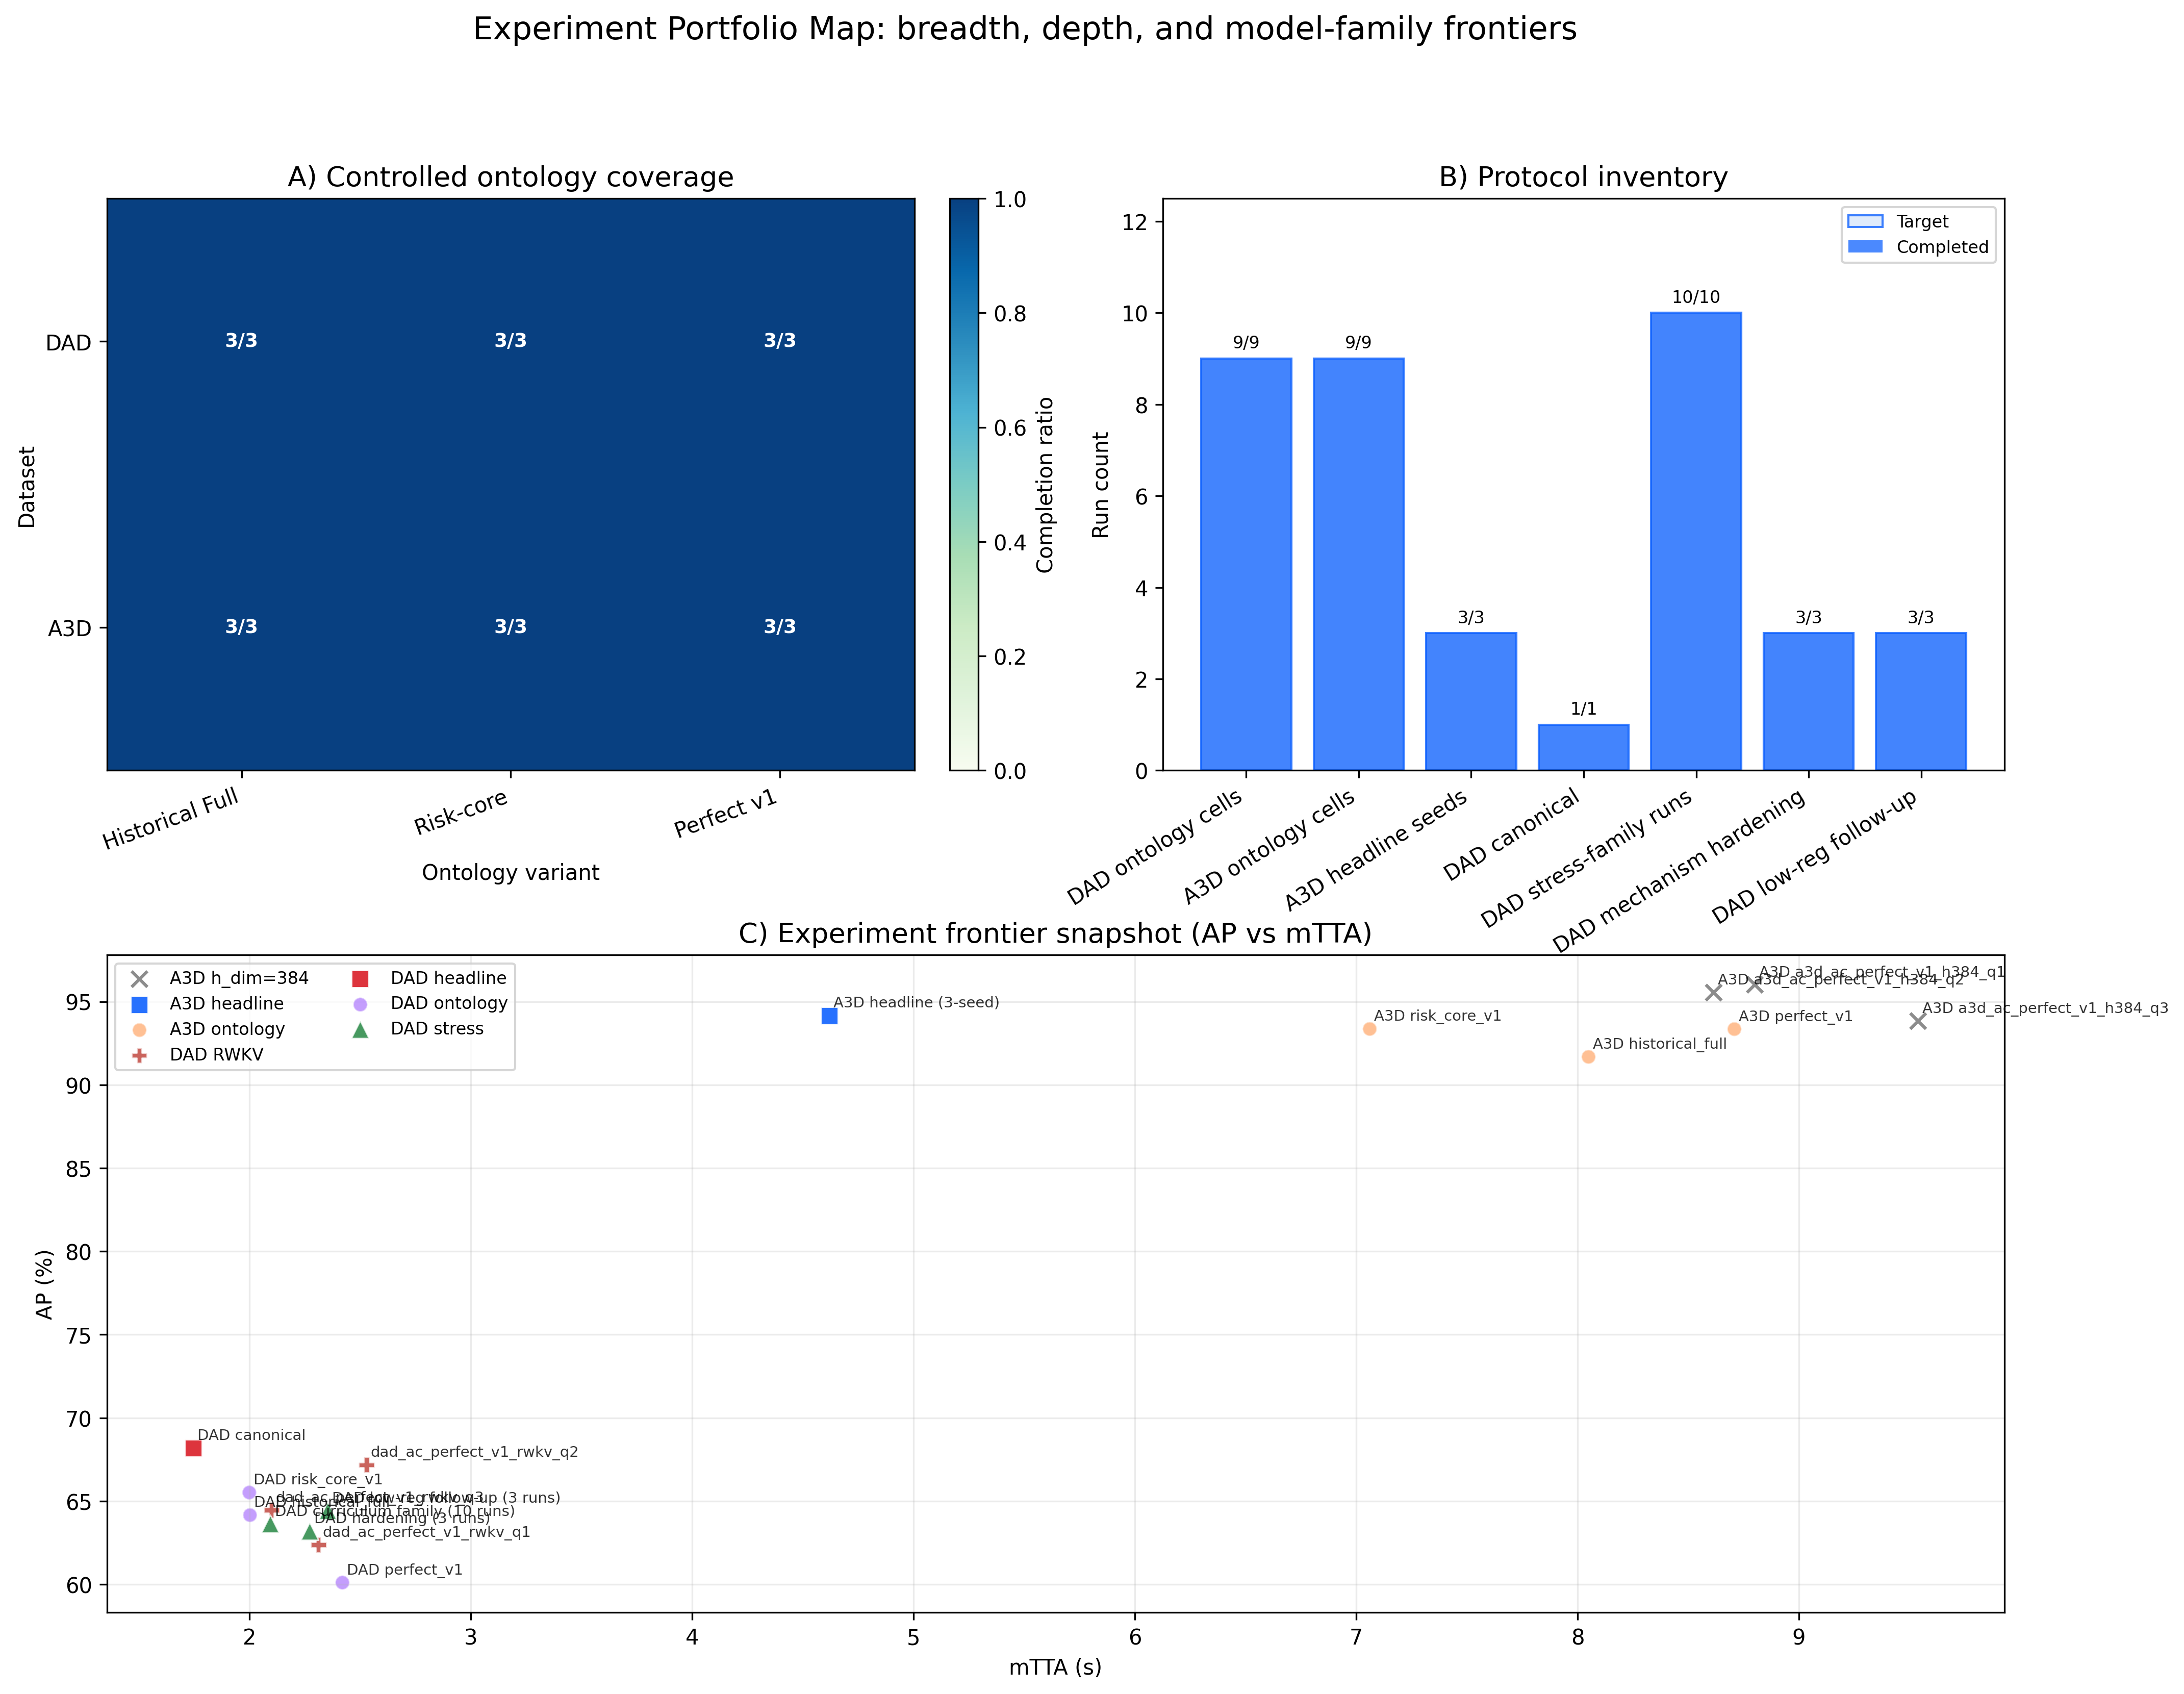
\includegraphics[width=0.98\textwidth]{../figures/insight_fig9_experiment_portfolio.pdf}
\caption{[Reading-map evidence] Experiment portfolio map used for claim-tier reading. Panel A
shows completion ratios for the controlled ontology matrix (DAD/A3D $\times$
three ontology variants). Panel B summarizes protocol depth by evidence family.
Panel C places headline, ontology, stress, and architecture-extension runs on
the same AP--mTTA plane. The figure makes execution coverage explicit without
mixing support evidence into headline claims.}
\label{fig:experiment_portfolio}
\end{figure*}
\subsection{Visual evidence upgrade: intervention gallery (support-only)}
\label{sec:intervention-gallery}
\begin{figure*}[t]
\centering
\begin{subfigure}{0.323\textwidth}
  \centering
  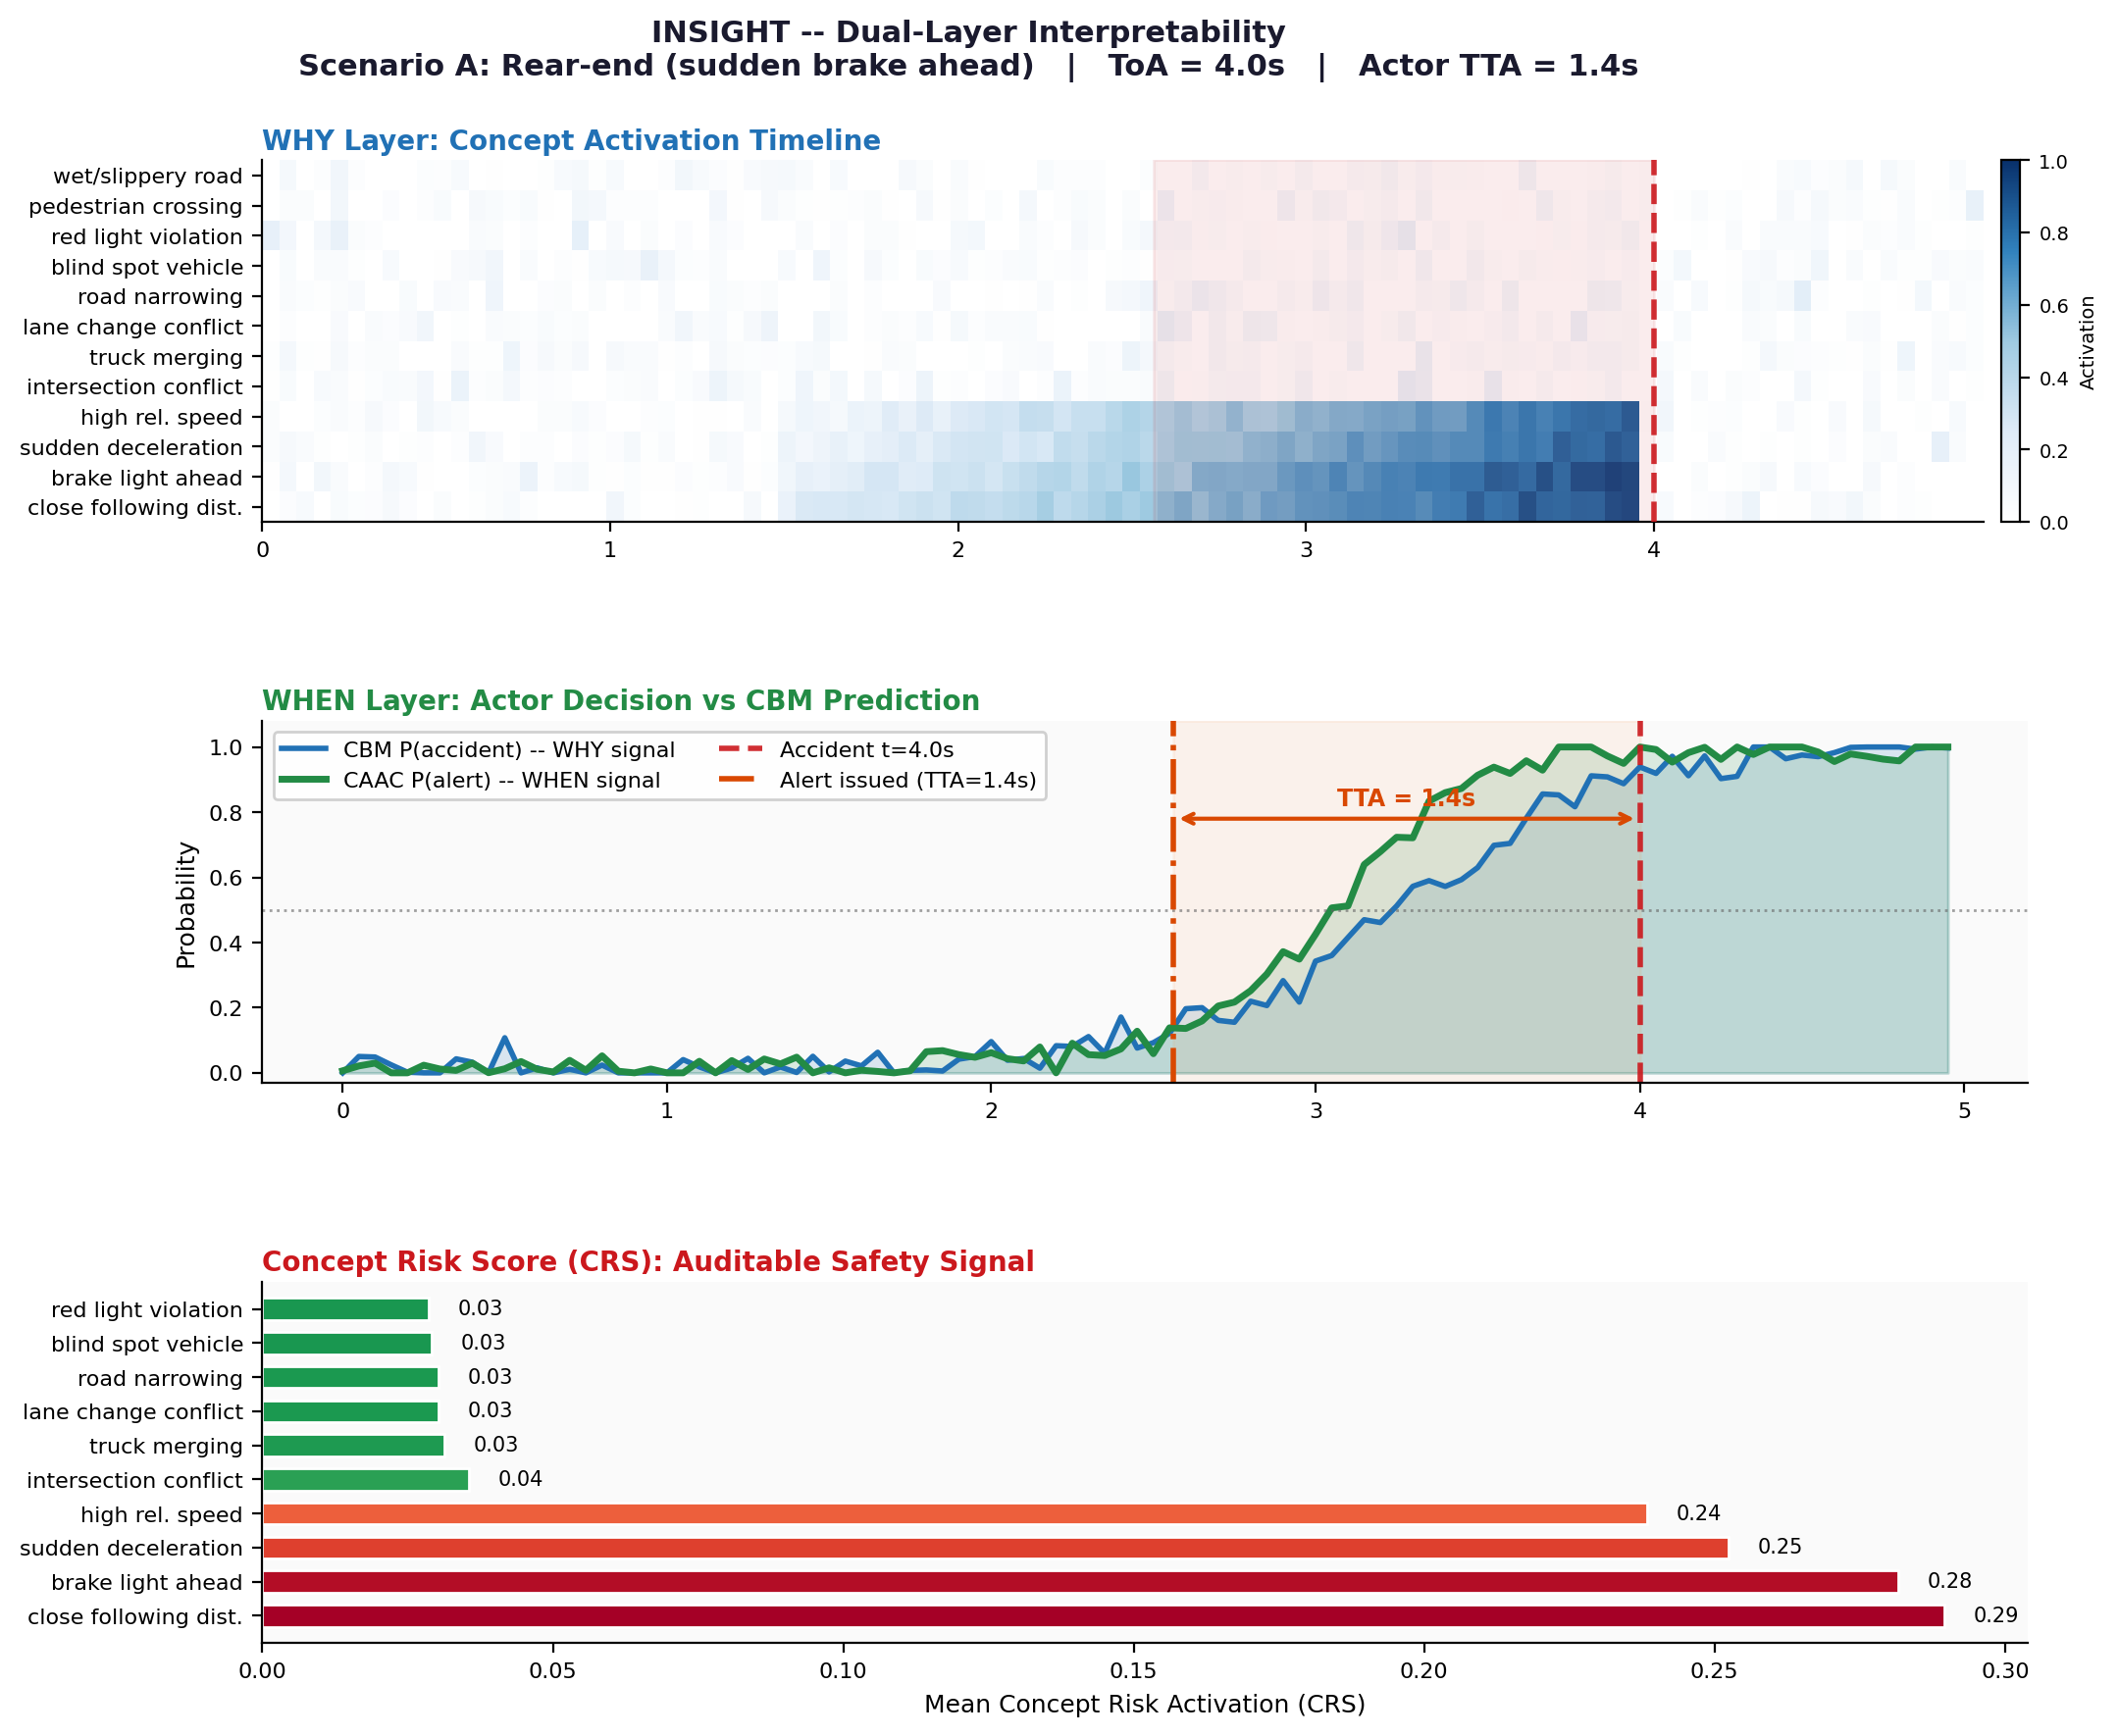
\includegraphics[width=\linewidth]{../figures/dual_interp_case1.png}
  \caption{Case 1}
\end{subfigure}
\hfill
\begin{subfigure}{0.323\textwidth}
  \centering
  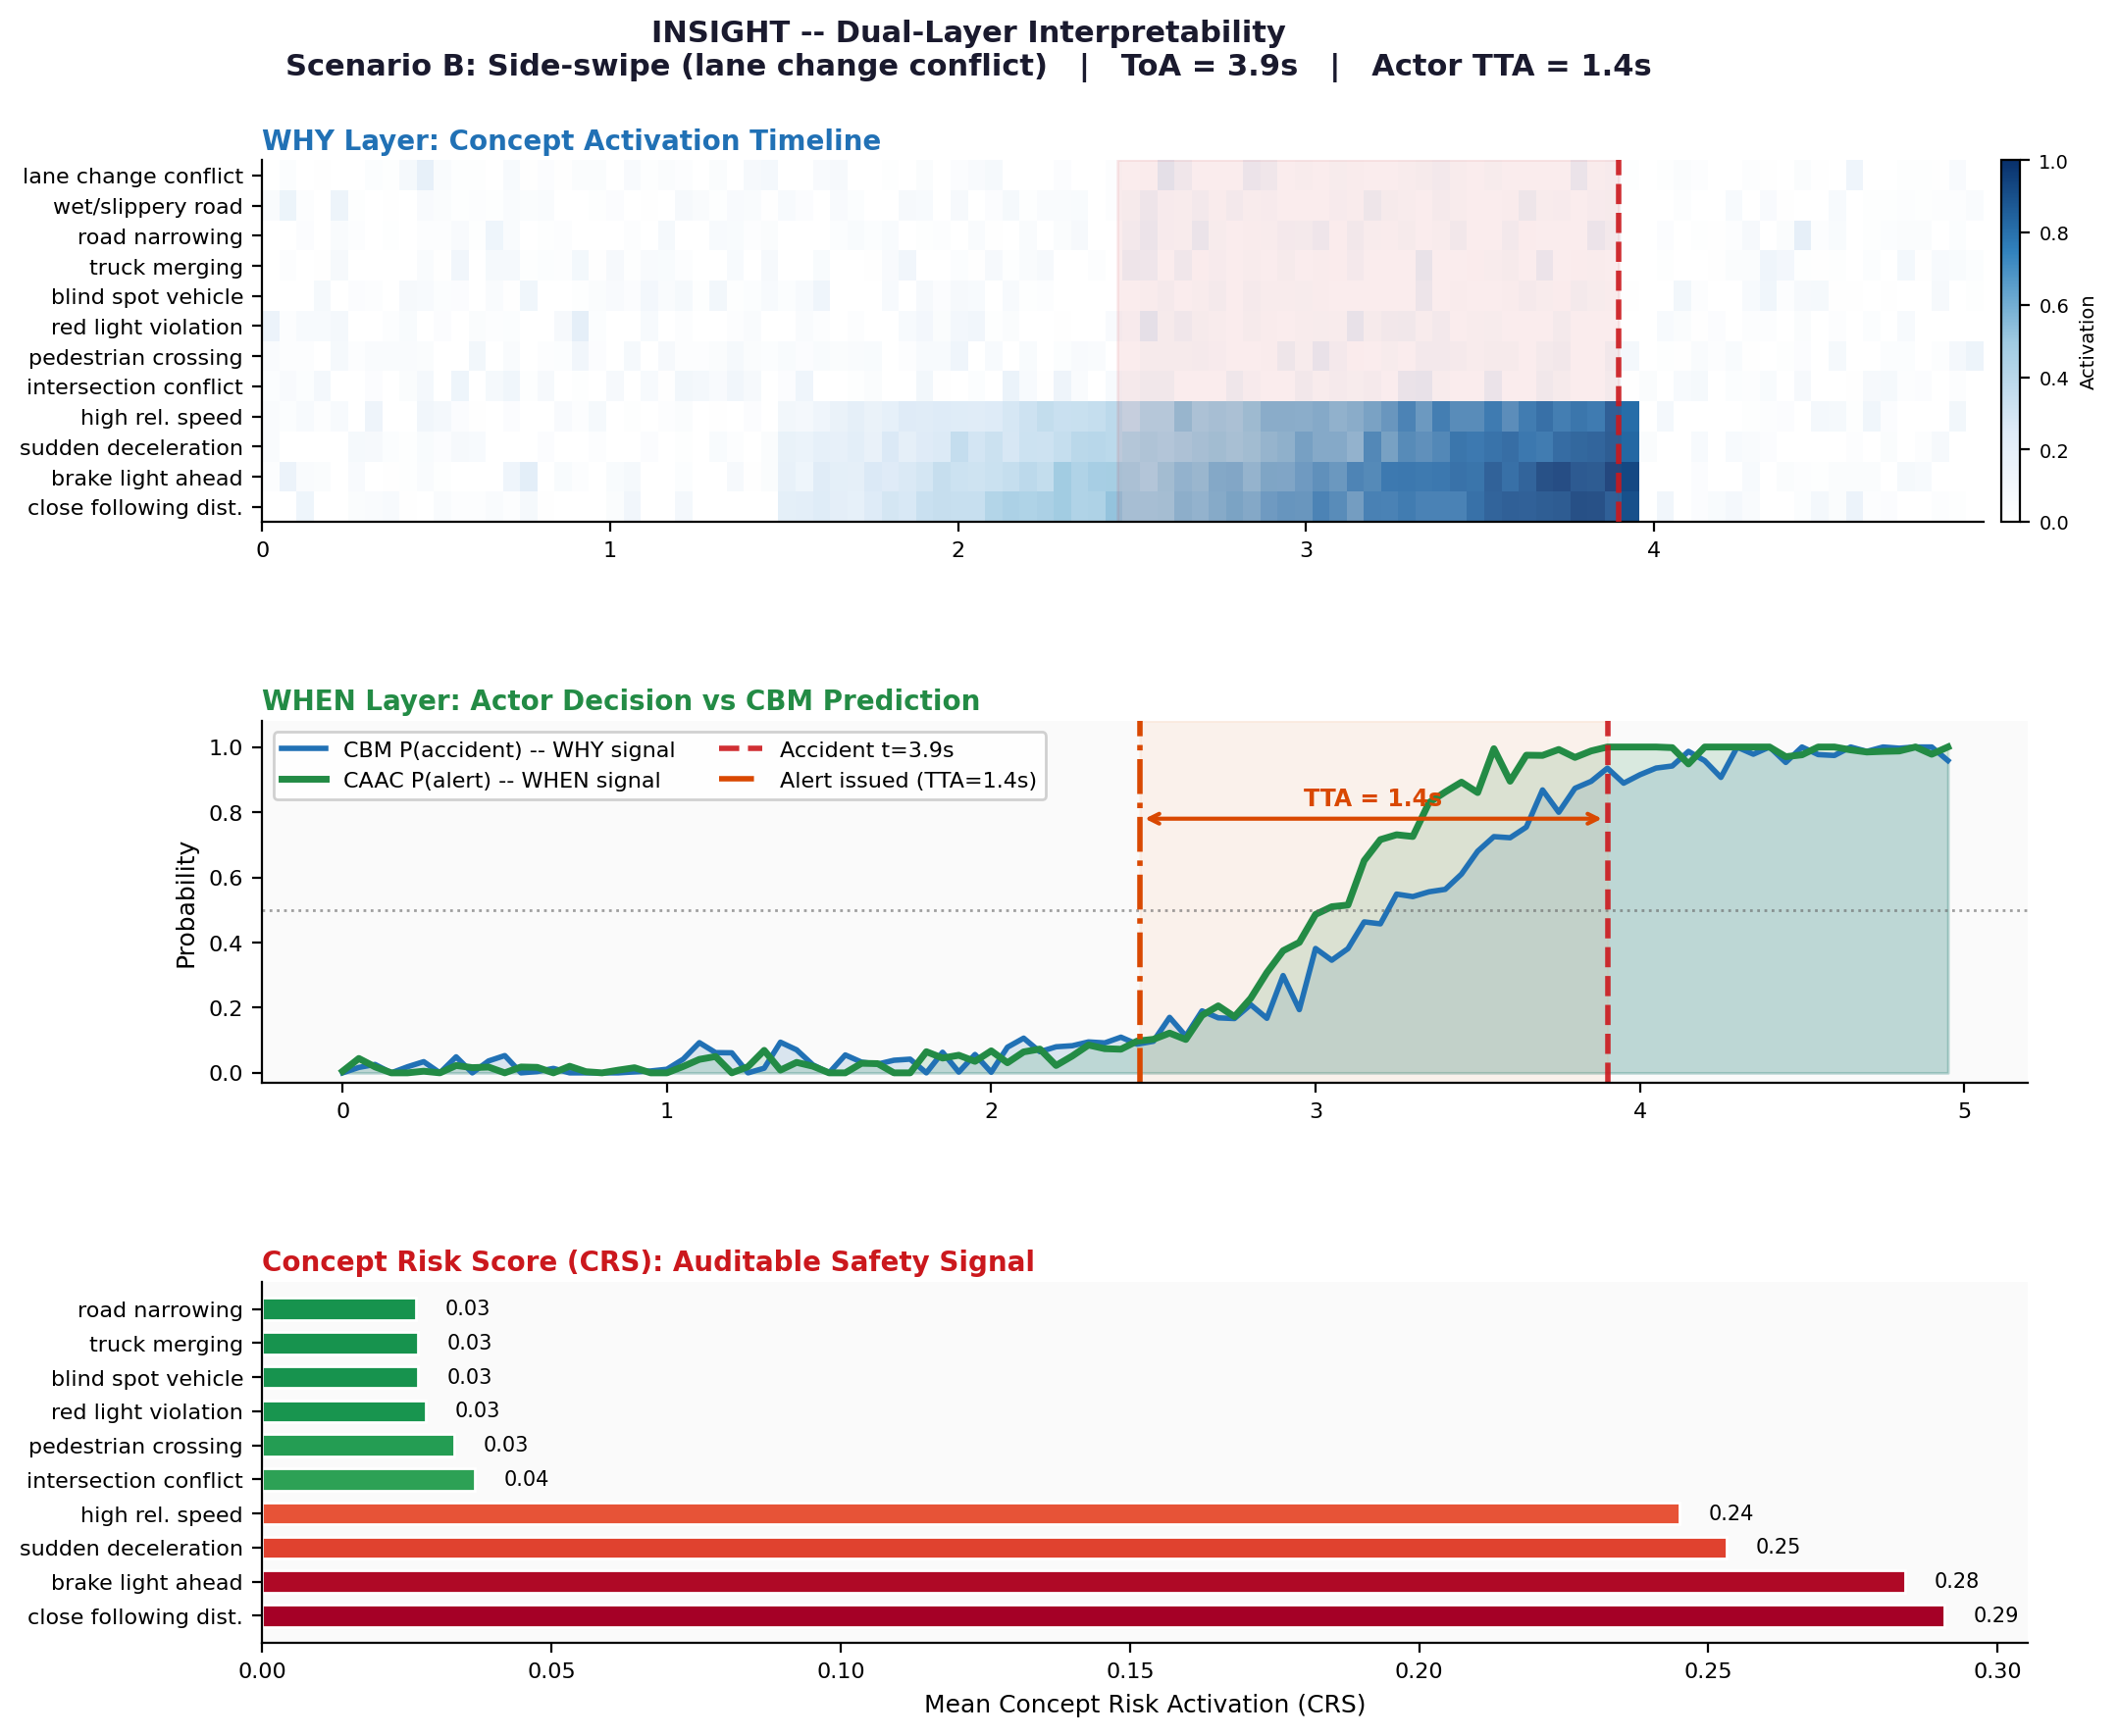
\includegraphics[width=\linewidth]{../figures/dual_interp_case2.png}
  \caption{Case 2}
\end{subfigure}
\hfill
\begin{subfigure}{0.323\textwidth}
  \centering
  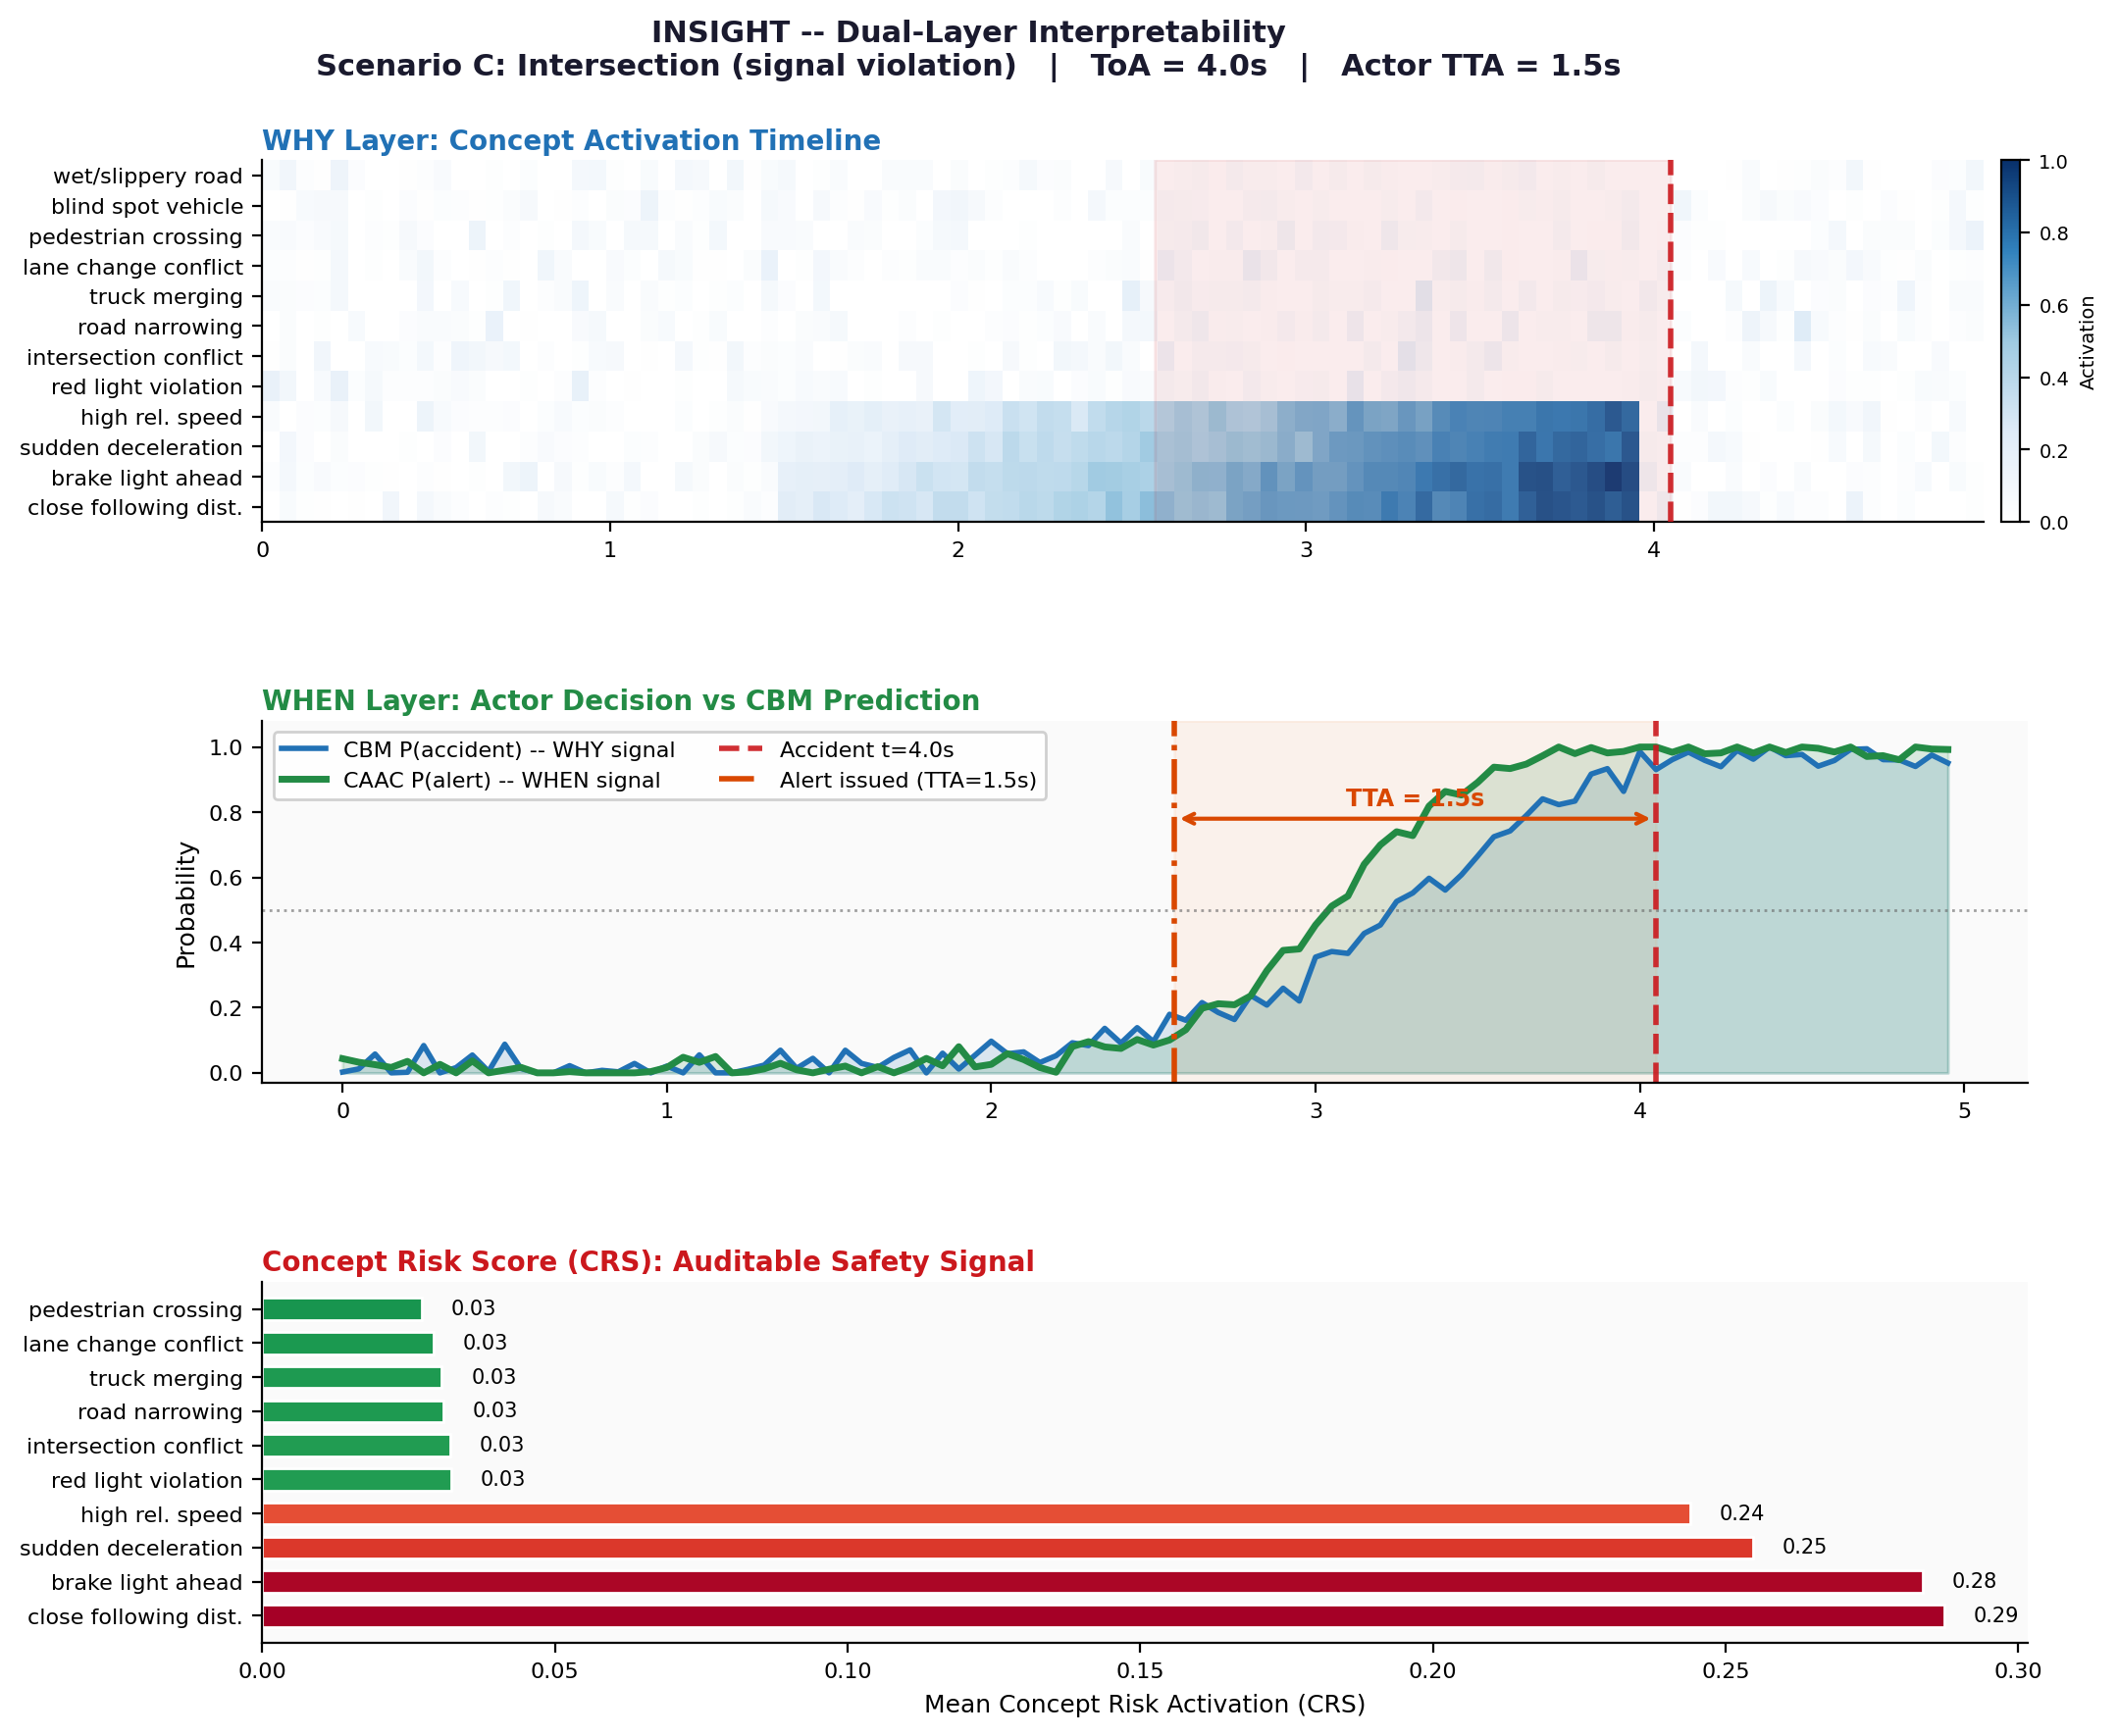
\includegraphics[width=\linewidth]{../figures/dual_interp_case3.png}
  \caption{Case 3}
\end{subfigure}
\caption{Support-only intervention gallery. The three paired DAD cases show how concept edits
alter activation trajectories under the same ontology protocol and where timing effects
do and do not change direction. It is intended as mechanistic intuition, not a headline result.}
\label{fig:intervention_gallery}
\end{figure*}

\begin{figure*}[t]
\centering
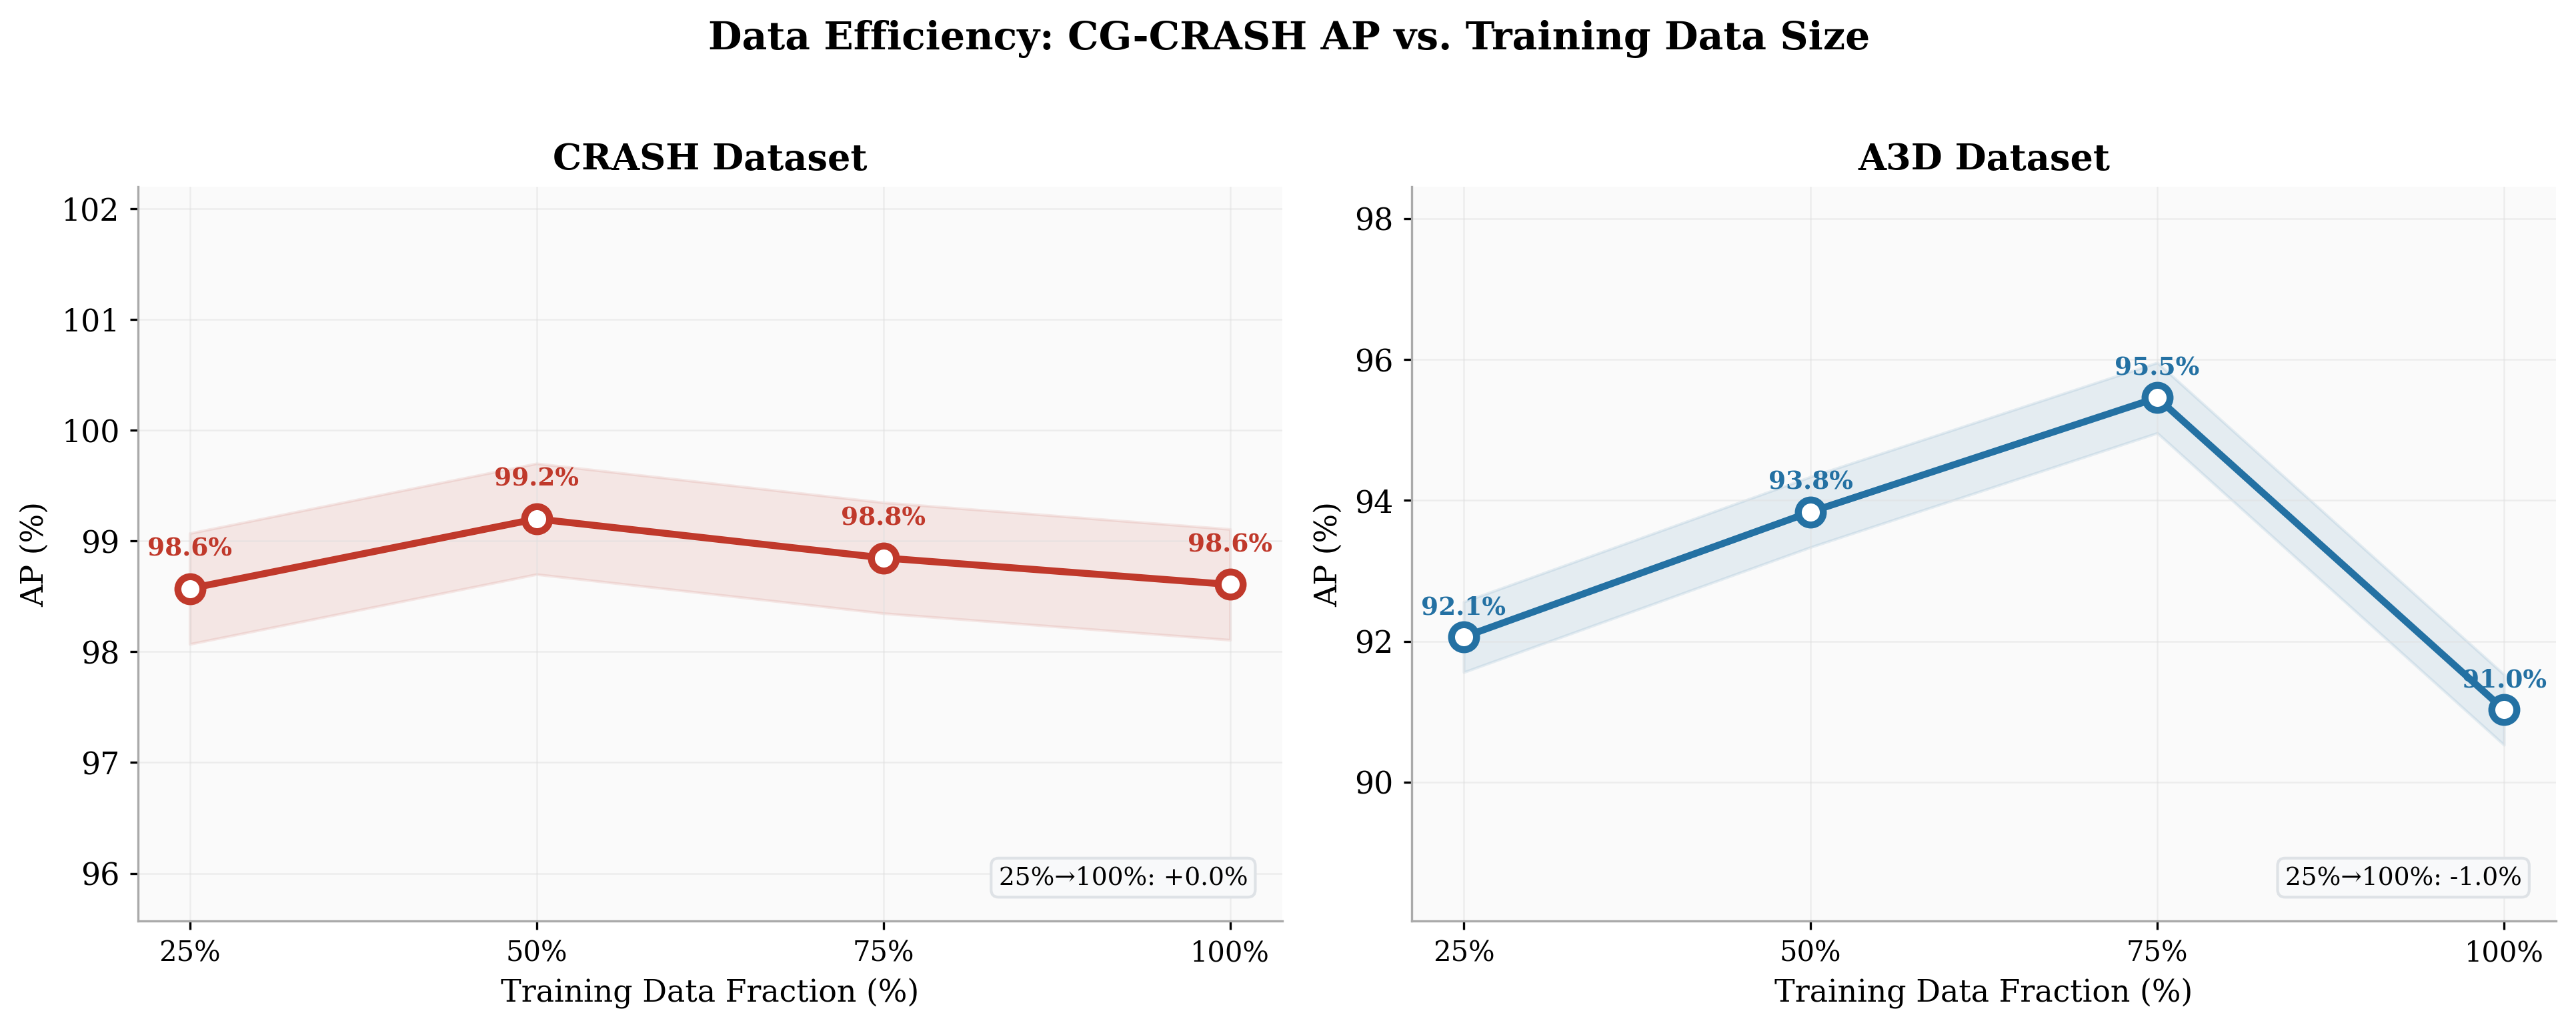
\includegraphics[width=0.98\textwidth]{../figures/insight_fig7_data_efficiency.pdf}
\caption{Cross-regime robustness check from data-fraction probes on CRASH, DAD, and
A3D. Broader dataset behavior is compared in the same protocol family, while
headline claims remain scoped by the tabulated results.}
\label{fig:data_efficiency}
\end{figure*}

\begin{figure*}[t]
  \centering
  \begin{subfigure}{0.495\textwidth}
    \centering
    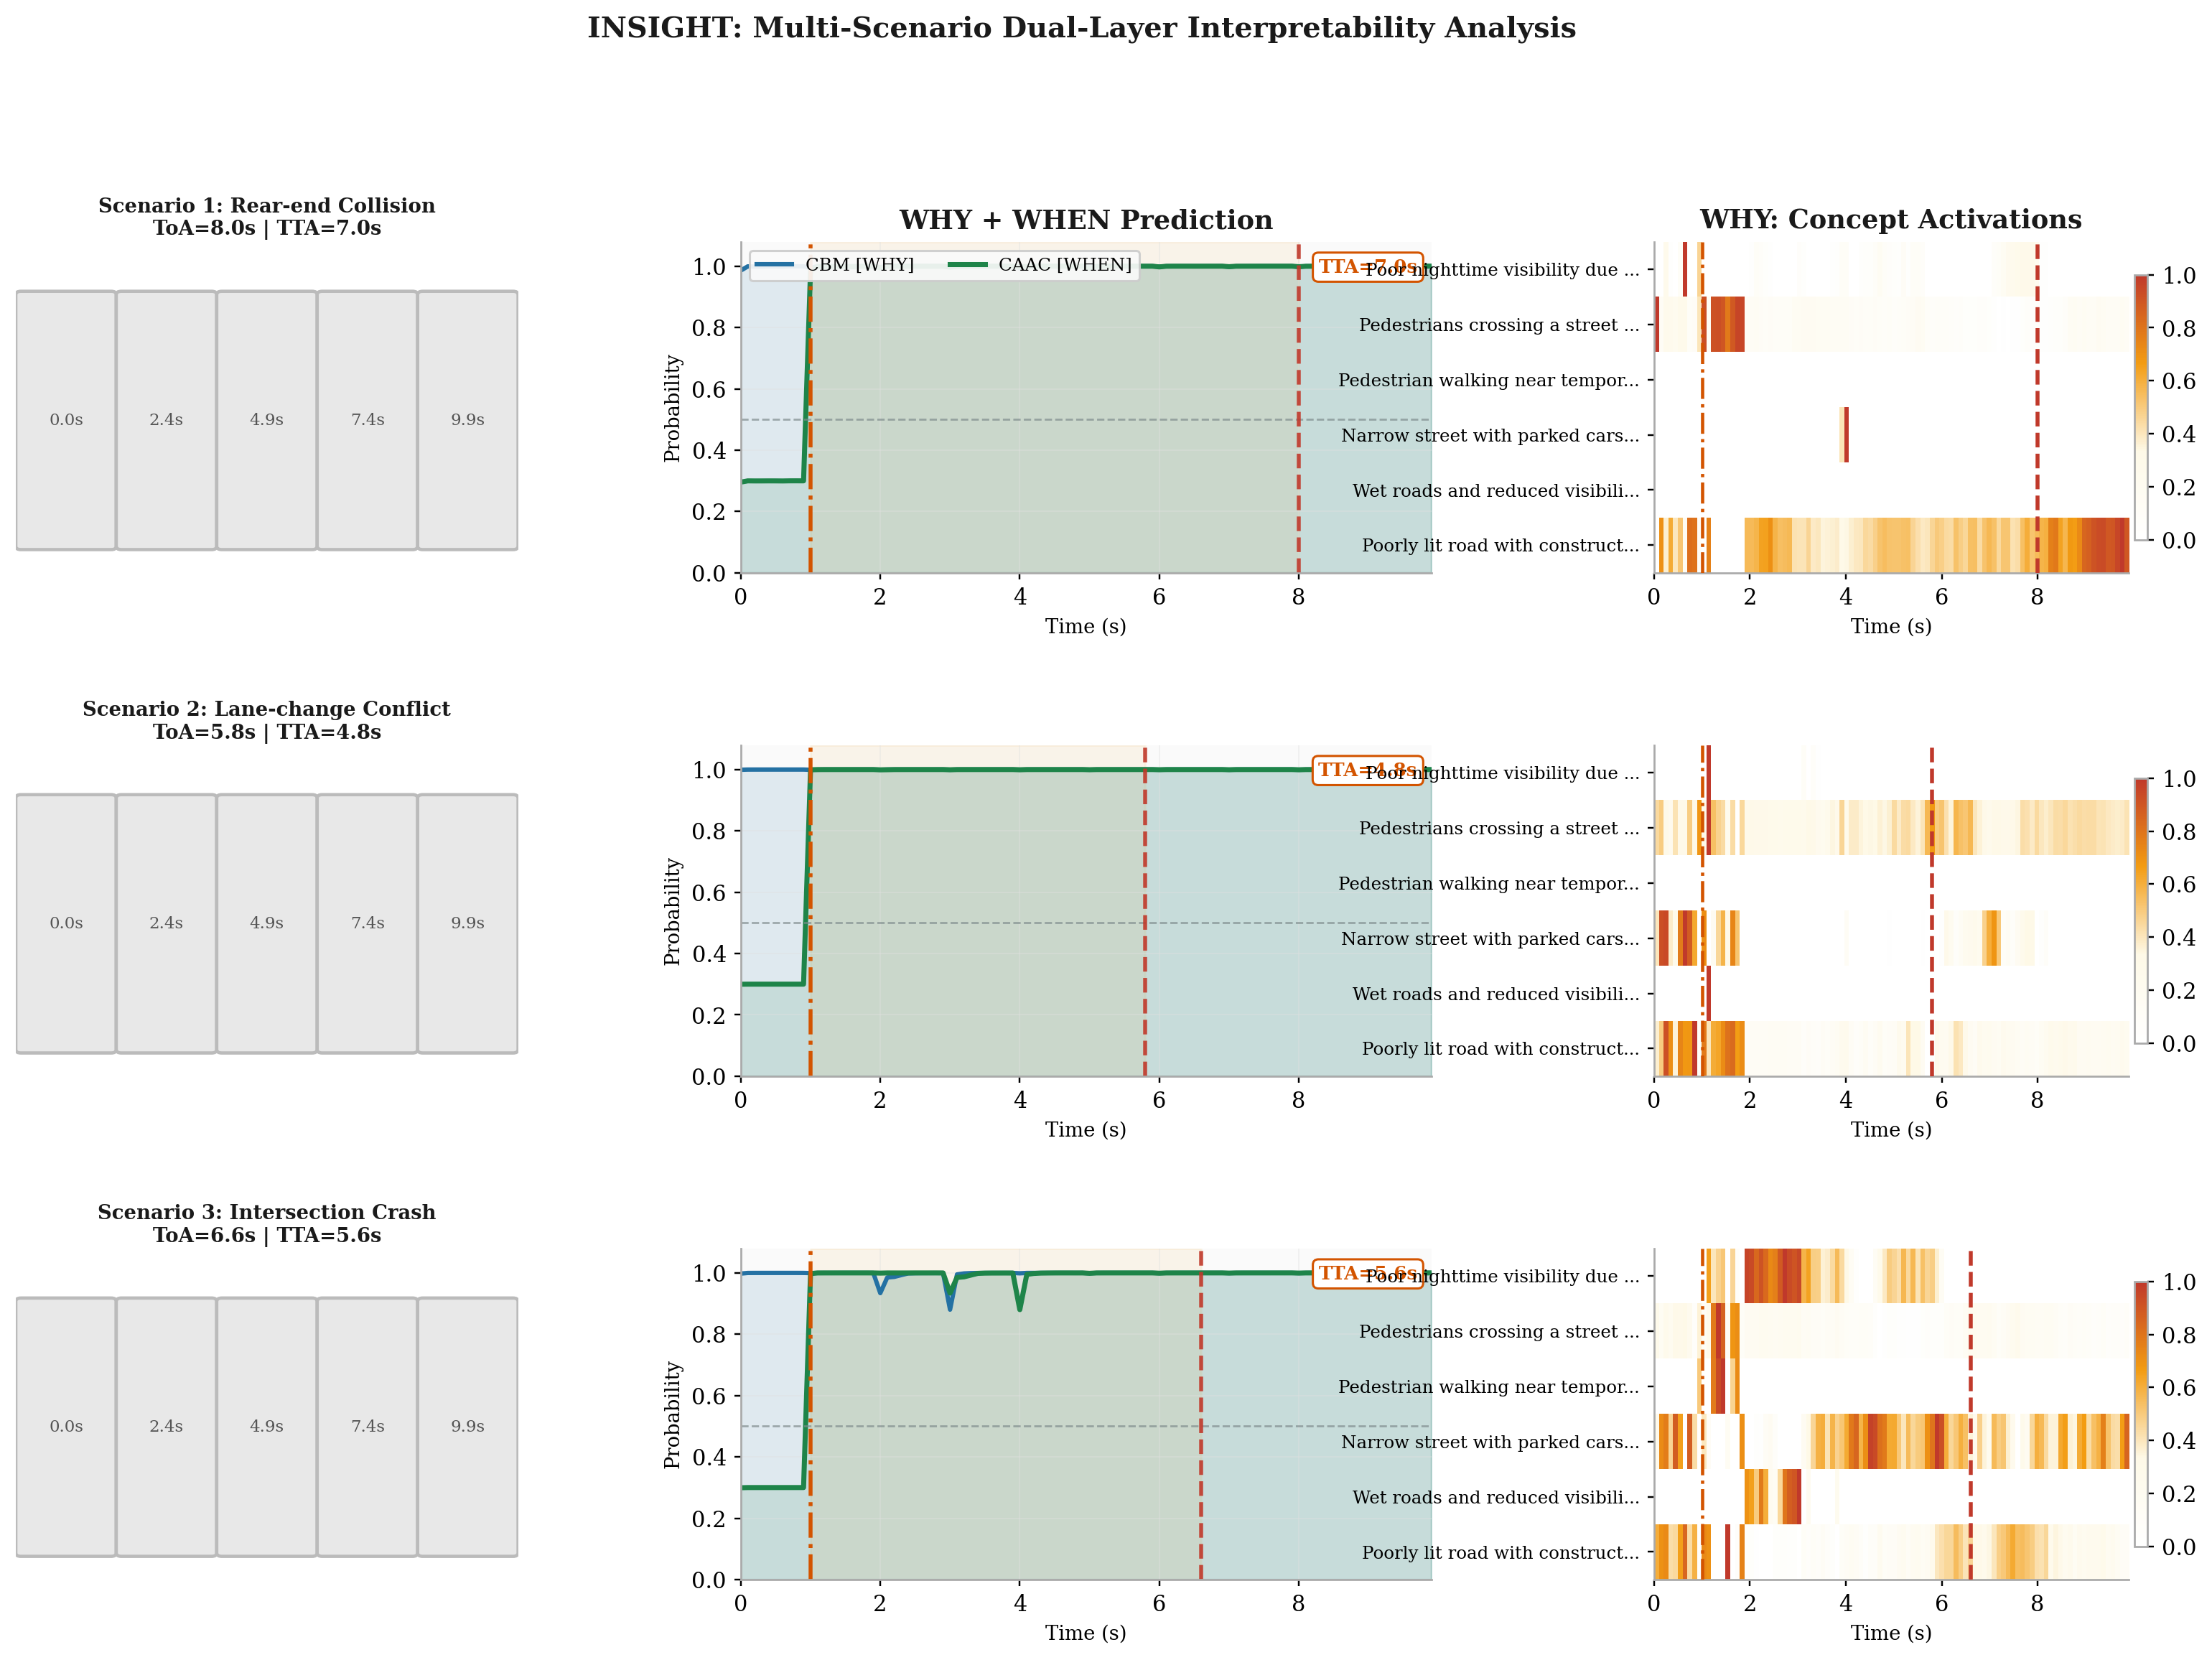
\includegraphics[width=\linewidth]{../figures/insight_fig2_multi_a3d.png}
    \caption{A3D representative trajectory}
    \label{fig:qual_case_a3d}
  \end{subfigure}
  \hfill
  \begin{subfigure}{0.495\textwidth}
    \centering
    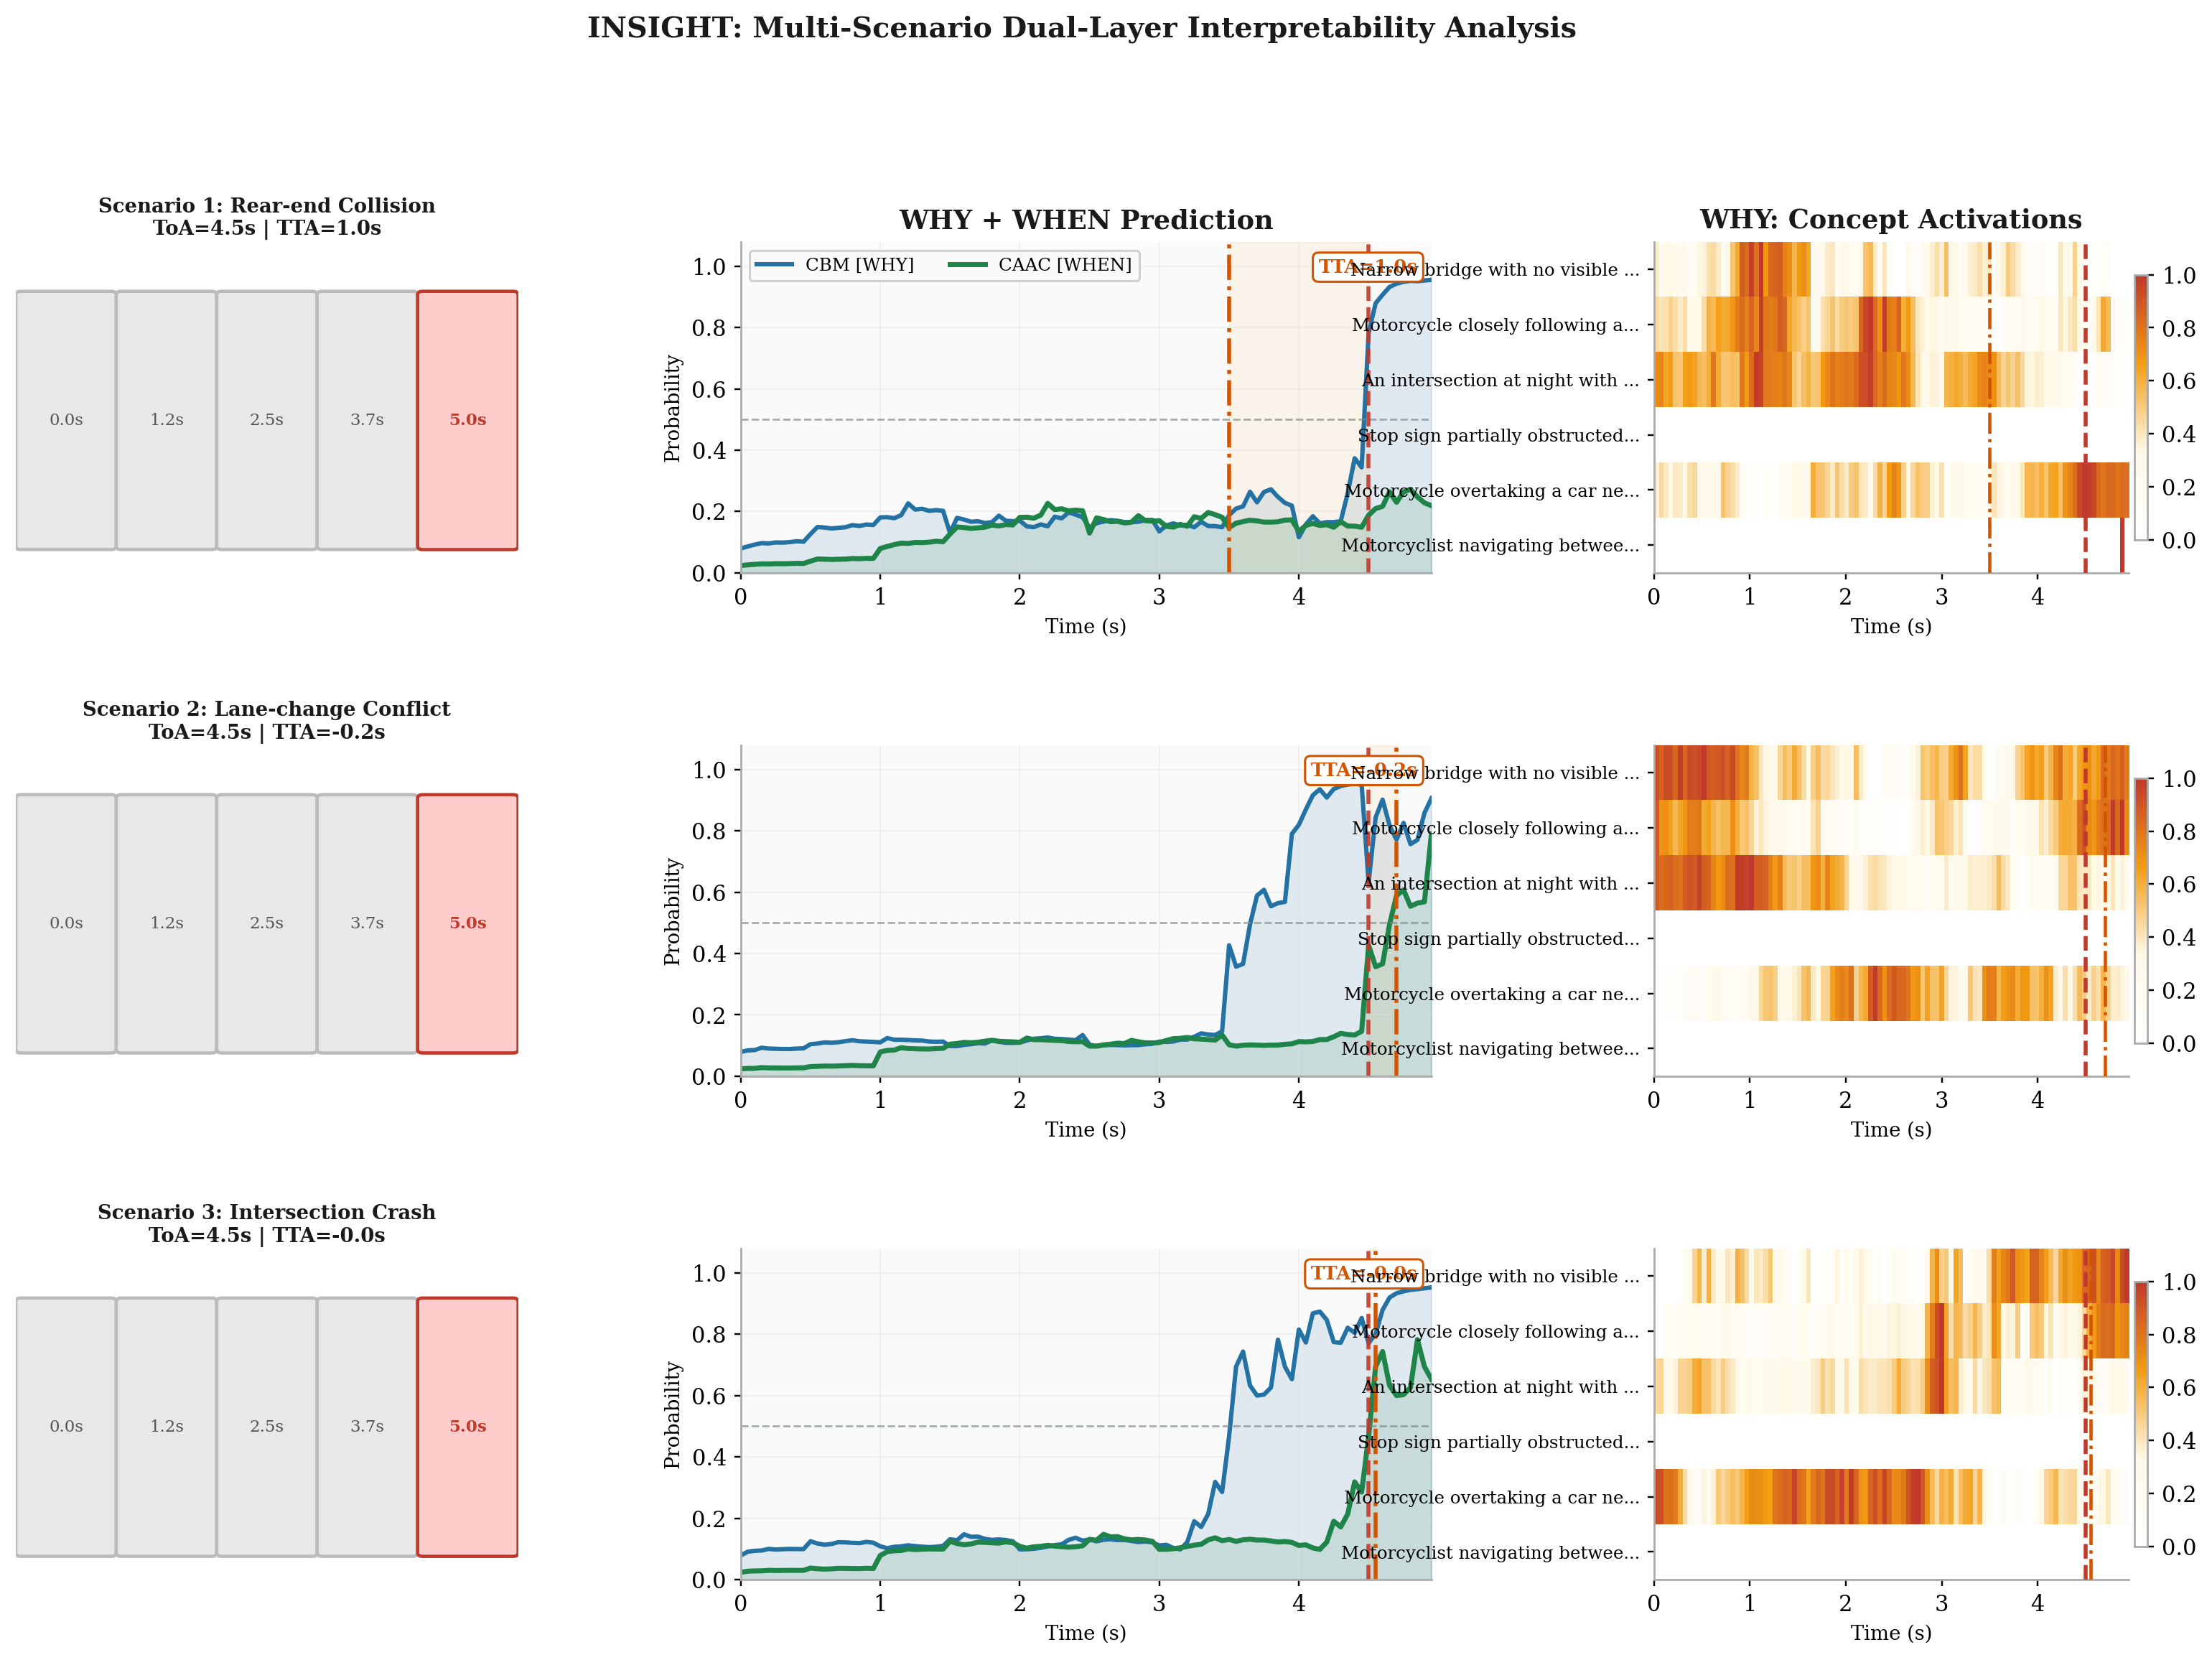
\includegraphics[width=\linewidth]{../figures/insight_fig2_multi_dad.png}
    \caption{DAD representative trajectory}
    \label{fig:qual_case_dad}
  \end{subfigure}
  \caption{Qualitative comparison of representative semantic traces. The two
  datasets show the same interface in different stress regimes: A3D exposes longer,
  progressively unfolding precursor patterns, while DAD is shorter and noisier.
  The paper uses these in-place visual checks only as intuition support; headline
  claims still use the protocol-separated quantitative blocks.}
  \label{fig:qual_case_stress}
\end{figure*}

\begin{figure*}[t]
  \centering
  \begin{subfigure}{0.495\textwidth}
    \centering
    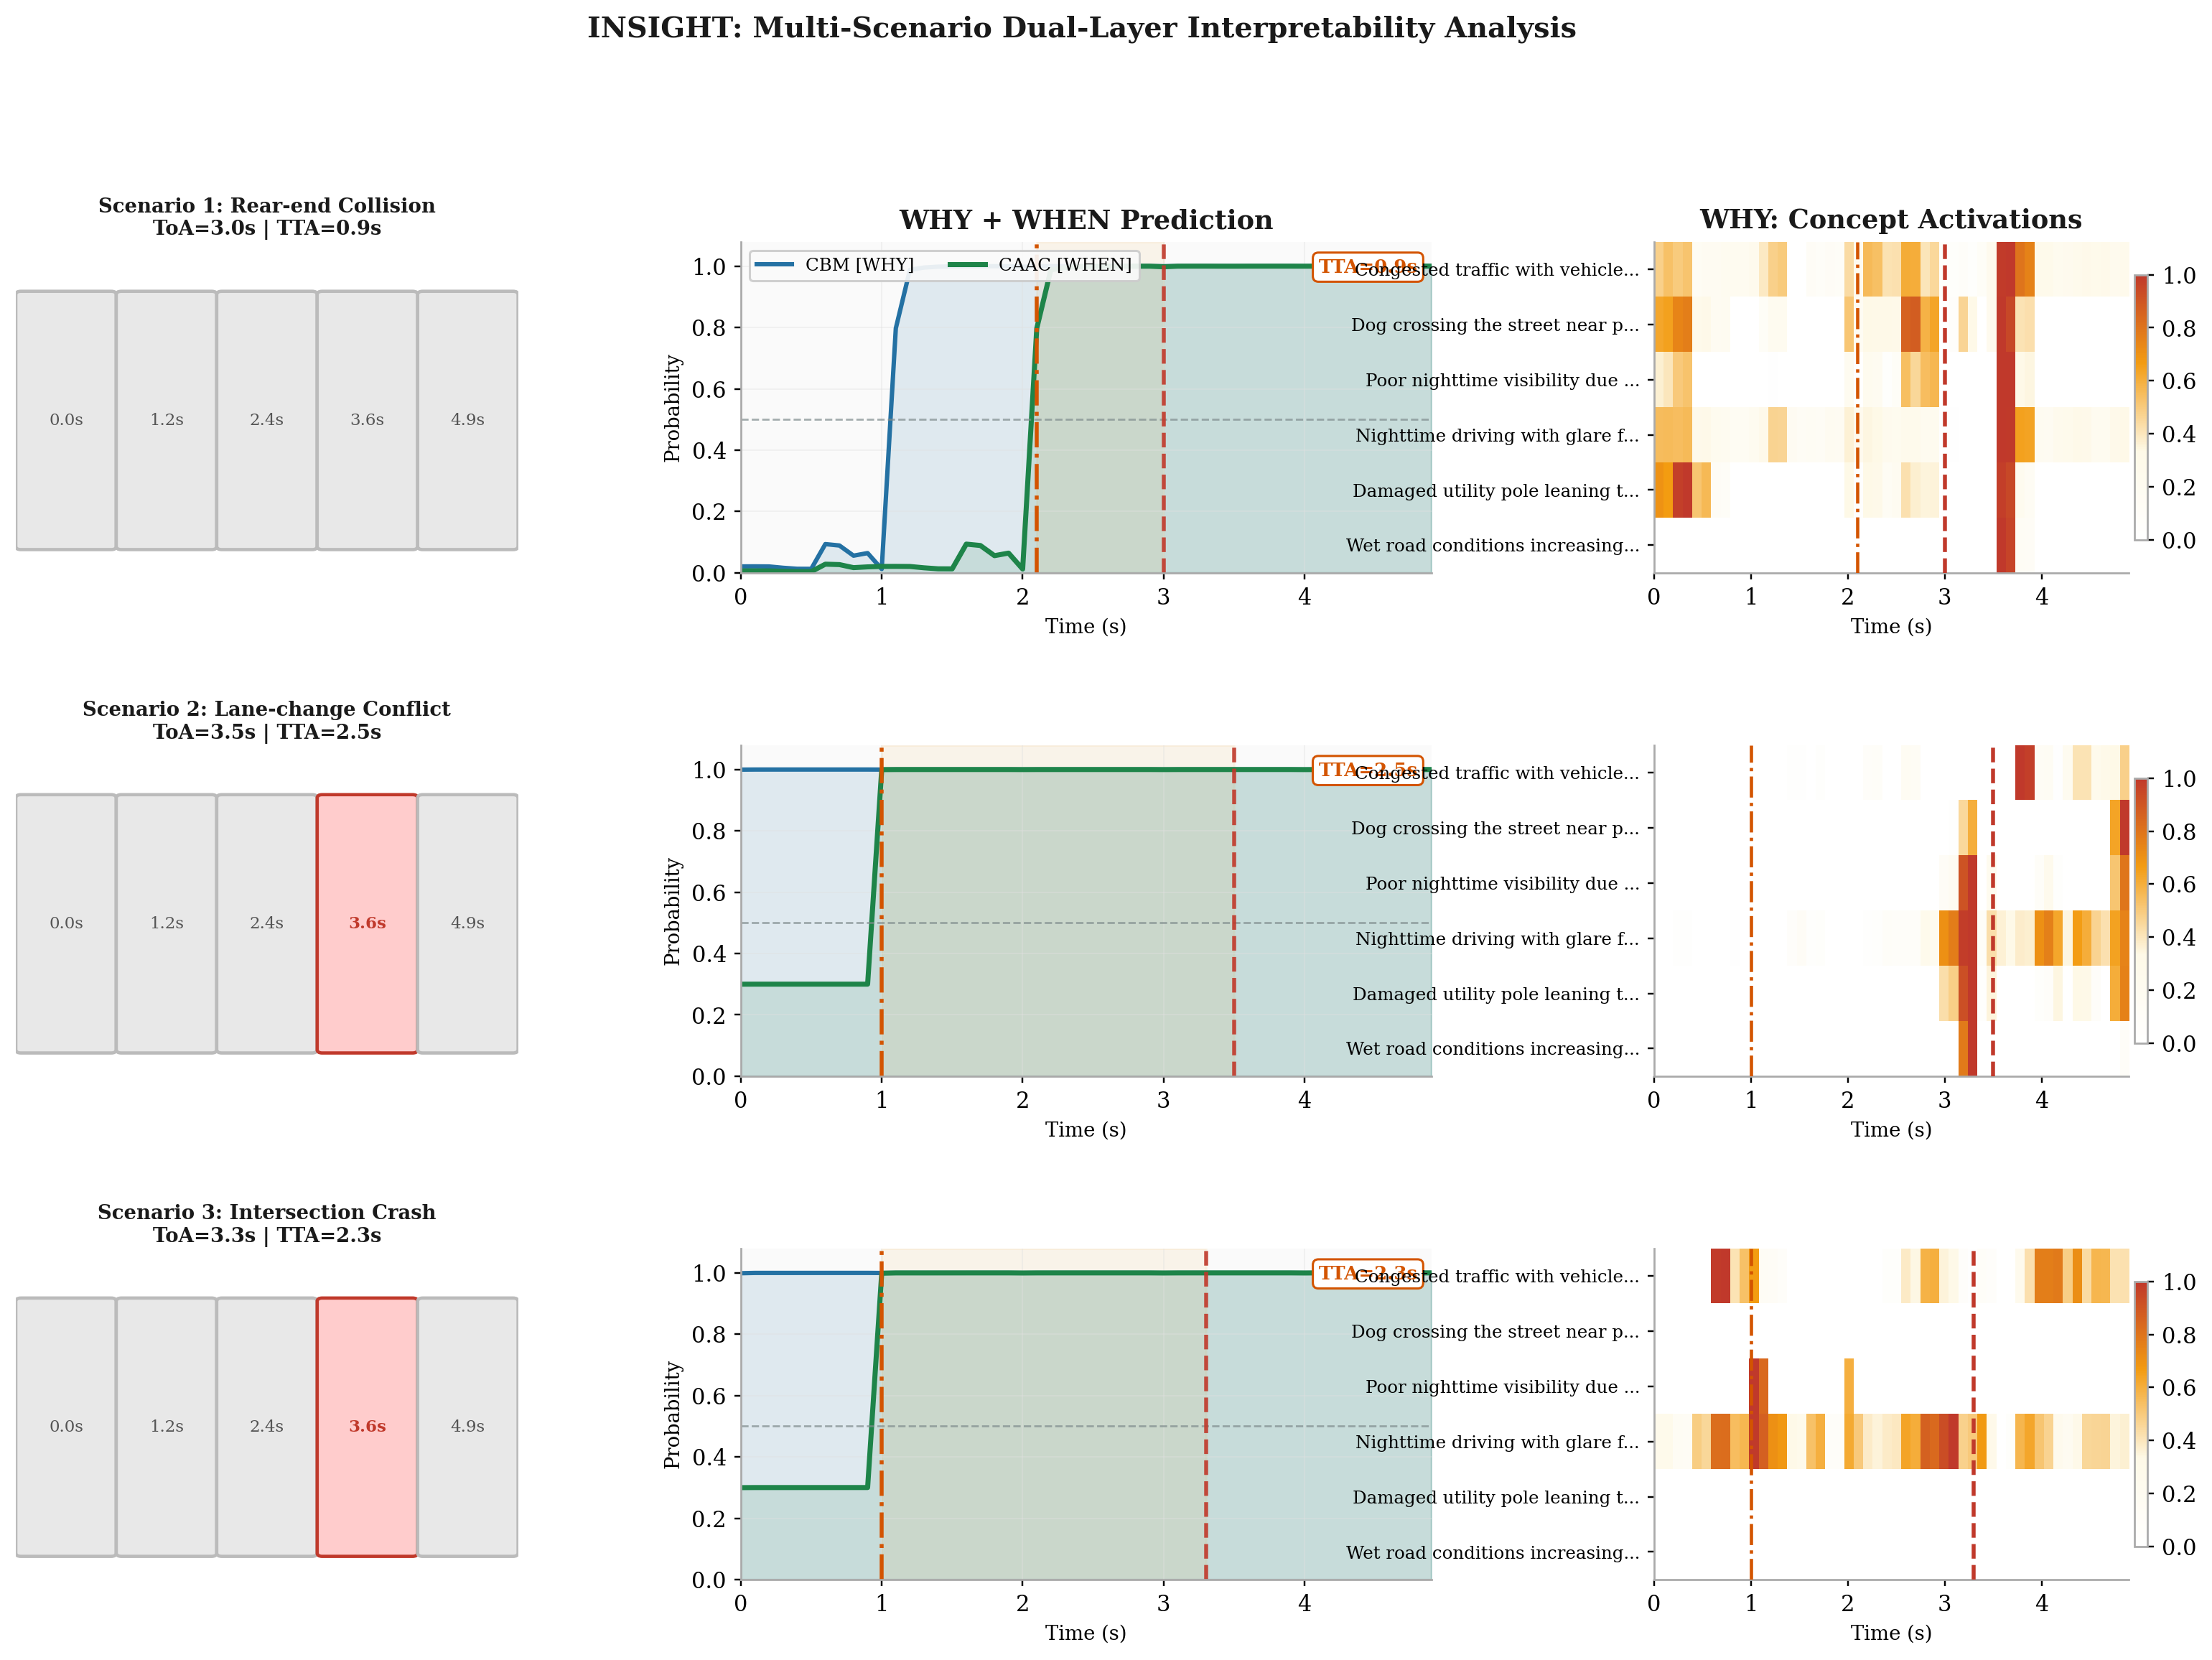
\includegraphics[width=\linewidth]{../figures/insight_fig2_multi_crash.png}
    \caption{CRASH representative trajectory}
    \label{fig:cross_dataset_bridge_traj}
  \end{subfigure}
  \hfill
  \begin{subfigure}{0.495\textwidth}
    \centering
    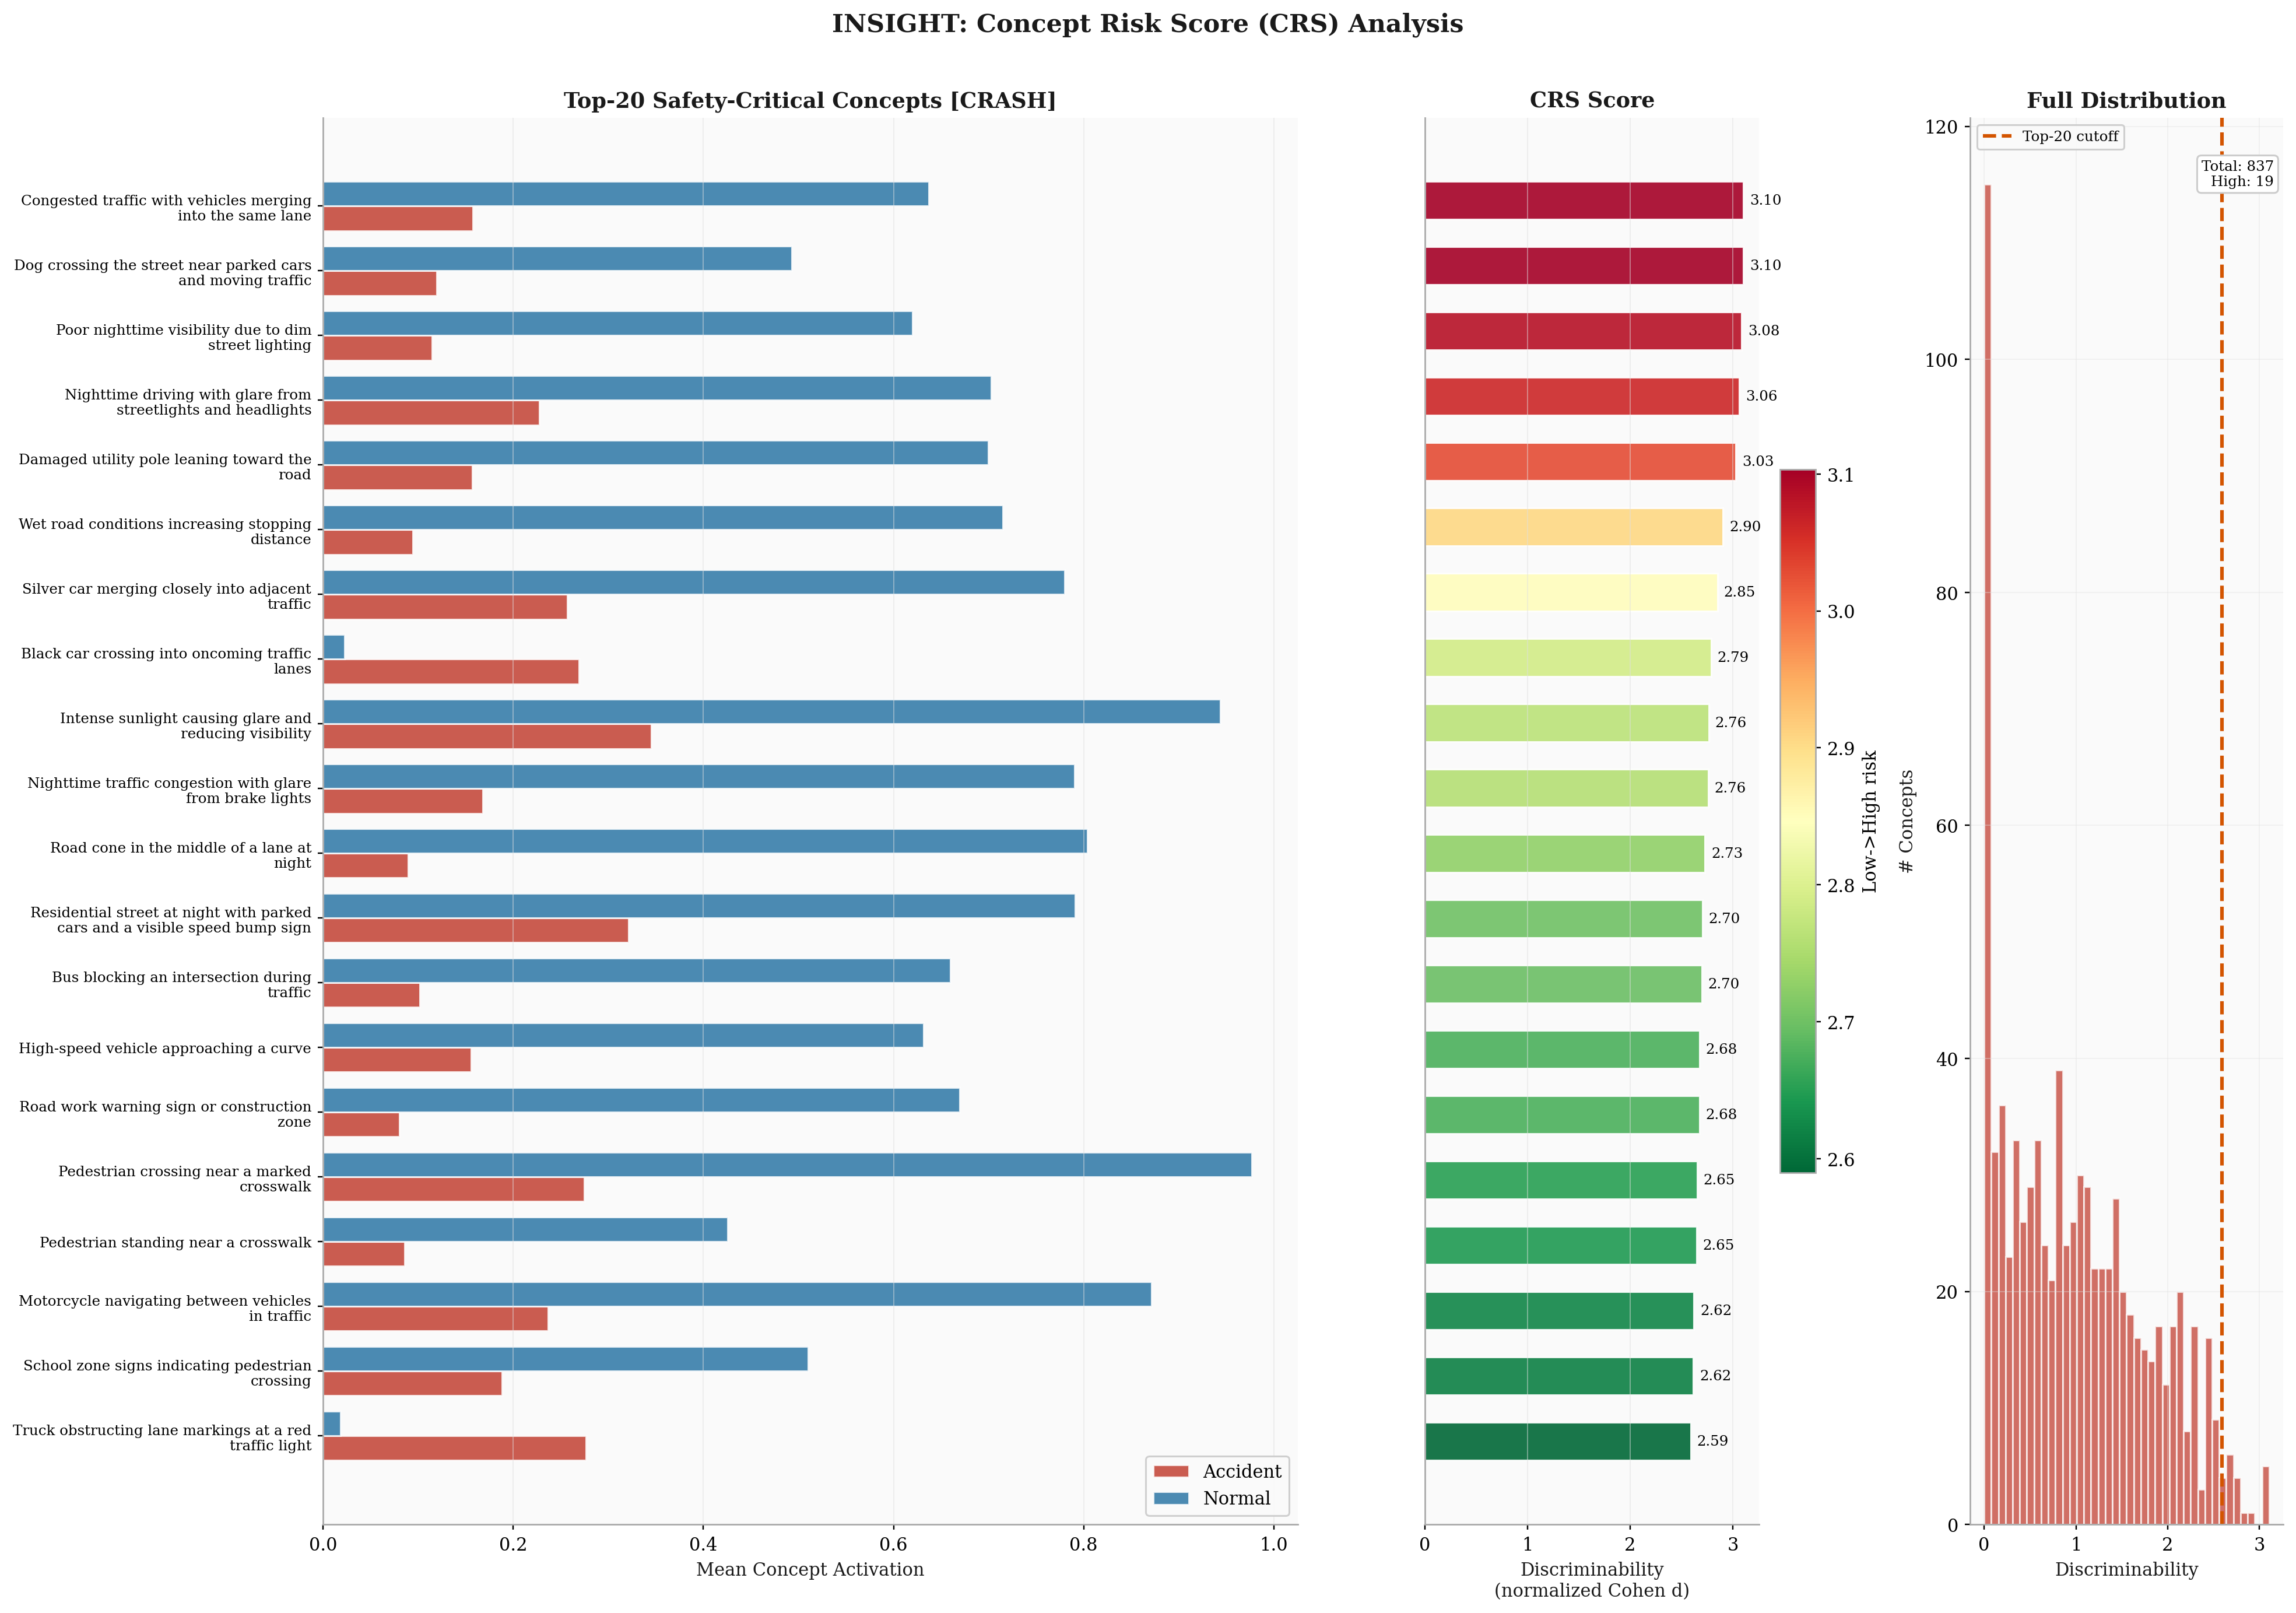
\includegraphics[width=\linewidth]{../figures/insight_fig3_crs_crash.png}
    \caption{CRASH CRS visualization}
    \label{fig:cross_dataset_bridge_crs}
  \end{subfigure}
  \caption{Cross-dataset stress bridge (support-only): CRASH cases illustrate how
  the semantic interface appears under a third corpus. These visual artifacts are
  treated as stress evidence only; headline claims remain scoped to DAD and A3D.}
  \label{fig:cross_dataset_bridge}
\end{figure*}

\paragraph{Scope and evidence envelope.}
The evaluation is deliberately designed around two datasets, not a large model
benchmark zoo. DAD and A3D are the explicit evidence corpus:
(\emph{i}) DAD serves as a noisy, short-horizon stress regime where fragility
is expected and tracked, and
(\emph{ii}) A3D serves as the cleaner regime where a semantic interface can be
interpreted as the flagship mechanism trajectory.
We do not claim dataset-agnostic dominance from this package; we claim
dataset-dependent behavioral control through a governed ontology.
\paragraph{Cross-dataset transfer note (support-only).}
To strengthen visual evidence depth, we keep one additional CRASH transfer check
as support evidence only. The archived CRASH transfer and phase-2 ablation
result files are intentionally interpreted as breadth stress signals and are not
pooled with headline DAD/A3D tables.

\subsection{Reviewer-Facing Evidence Map}
\label{sec:review-map}
\begin{figure*}[t]
\centering
\setlength{\fboxsep}{6pt}
\fbox{%
\begin{minipage}[t]{0.31\textwidth}
\textbf{Headline evidence}\\
\textbf{Use:} fast accept-level comparison\\
\textbf{Main artifacts:} Table~\ref{tab:dad}, Table~\ref{tab:a3d}, Figure~\ref{fig:safety_utility}\\
\textbf{Reading:} A3D is the clean flagship operating point; DAD headline is reported but not overstated.
\end{minipage}}
\hfill
\fbox{%
\begin{minipage}[t]{0.31\textwidth}
\textbf{Controlled support evidence}\\
\textbf{Use:} test ontology/mechanism under matched launchers\\
\textbf{Main artifacts:} Table~\ref{tab:concept_sets}, Table~\ref{tab:ablation}, Figure~\ref{fig:qual_case_stress}\\
\textbf{Reading:} ontology choice is an empirical variable; support blocks are not pooled as leaderboard claims.
\end{minipage}}
\hfill
\fbox{%
\begin{minipage}[t]{0.31\textwidth}
\textbf{Stress evidence}\\
\textbf{Use:} boundary and failure-mode disclosure\\
\textbf{Main artifacts:} DAD robustness paragraphs, Table~\ref{tab:interp_quant}, appendix intervention logs\\
\textbf{Reading:} DAD remains fragile stress evidence; actor-policy timing remains scoped support.
\end{minipage}}
\caption{[Reading-map evidence] Visual evidence map for rapid claim-tier reading. The paper separates
headline, controlled support, and stress evidence so each claim has one role
and one interpretation tier.}
\label{fig:review_map}
\end{figure*}

\paragraph{Pseudo-label sensitivity.}
We also audited the top-$m$ CLIP pseudo-label recipe on a larger 500-frame DAD
slice from the paper ontology. The main takeaway remains pragmatic: top-3 is a
reasonable middle ground. In this audit, top-1 activates only one semantic
family per frame on average and captures 5.5\% of the cumulative top-20
similarity mass, while top-10 spreads across 5.14 families and absorbs 51.5\%
of that mass. Top-3 sits between these extremes with 2.34 families per frame
and 16.0\% relative mass, so we retain it in the main recipe as a practical
balance between coverage and noise rather than as a claim of exact semantic
calibration.

\paragraph{Verbalization robustness.}
We also measured whether canonical paper-facing concept names remain stable
under light paraphrase changes. Across 12 canonical concepts with two variants
each, canonical and variant prompts achieve mean text cosine 0.939, mean
frame-score correlation 0.887, mean top-10 frame overlap 0.525, and mean
absolute score difference 0.013 on the same 500-frame DAD audit. These results
support the paper's naming policy: short canonical risk phrases remain stable
anchors for the semantic interface, even though a few more abstract paraphrases
are visibly weaker.

Taken together, the pseudo-label and paraphrase audits address two different
language-side failure modes. The top-$m$ audit checks whether the semantic
bootstrap is too concentrated or too diffuse, while the paraphrase audit checks
whether the paper-facing ontology is brittle to minor wording changes. Together
with the family-balance and merge-provenance assets in the appendix, these
analyses justify treating the ontology as a governed language interface rather
than as a hidden prompt artifact.

\subsection{Interpretability Taxonomy of Prior Work}

\begin{table}[t]
\caption{[Controlled support evidence] Interpretability taxonomy for accident anticipation. The point of this
table is not that every method should expose the same type of explanation, but
that most prior systems still lack an explicit semantic interface that can be
trained, audited, and compared across runs.}
\label{tab:interp_comparison}
\centering\small
\setlength{\tabcolsep}{4pt}
\resizebox{\linewidth}{!}{%
\begin{tabular}{lcccc}
\toprule
Method & Semantic state & Timing account & Intrinsic? & Params\\
\midrule
DSA-RNN~\citep{ref4}         & \texttimes & \texttimes & -- & 12M\\
DRIVE~\citep{ref2}           & Grad-CAM & RL-trained attention & post-hoc & 31M\\
DSTA~\citep{ref17}           & \texttimes & \texttimes & -- & 180M\\
DAA-GNN~\citep{ref32}        & \texttimes & \texttimes & -- & 183M\\
W3AL~\citep{liao2024and}     & verbal localisation & verbal timing & post-hoc & 7B\\
CRASH~\citep{liao2024crash}  & \texttimes & \texttimes & -- & 26M\\
CCAF-Net~\citep{liu2025ccaf} & \texttimes & \texttimes & -- & 191M\\
LATTE~\citep{ZHANG2025103173}& \texttimes & \texttimes & -- & 45M\\
\midrule
\textbf{\method{} (Ours)} & \textbf{concept bottleneck} &
\textbf{concept-conditioned timing} & \textbf{\checkmark} & \textbf{30M}\\
\bottomrule
\end{tabular}%
}
\end{table}

Table~\ref{tab:interp_comparison} highlights the representational gap that
motivates our paper. Prior methods may be highly predictive, but most do not
provide a trainable semantic layer that links named risk concepts to downstream
anticipation behavior. \method{} closes that gap architecturally. Empirically,
the paper is strongest on the semantic layer and on ontology-controlled
comparisons, with timing analyses reported as a downstream extension of the
same interface.

\subsection{Main Predictive Results on DAD}

\begin{table}[t]
\caption{[Headline evidence] DAD results. We separate interpretable or
explanation-oriented methods
from strong non-interpretable references to position \method{} as a competitive
interpretable system with an explicit semantic interface.}
\label{tab:dad}
\centering\small
\setlength{\tabcolsep}{4pt}
\resizebox{\linewidth}{!}{%
\begin{tabular}{lcccc}
\toprule
Method & Venue & AP$\uparrow$ & mTTA$\uparrow$ & Interface\\
\midrule
DSA-RNN~\citep{ref4}        & ACCV'16 & 38.1\% & 2.05s & none\\
DRIVE~\citep{ref2}          & ICCV'21 & 58.4\% & 2.31s & post-hoc\\
DSTA~\citep{ref17}          & TITS'22 & 56.1\% & 3.66s & none\\
Graph$^2$~\citep{ref36}     & WACV'24 & 64.8\% & 2.98s & none\\
DAA-GNN~\citep{ref32}       & PR'24 & 75.2\% & 1.59s & none\\
W3AL~\citep{liao2024and}    & MM'24 & 69.2\% & -- & verbal\\
CRASH~\citep{liao2024crash} & MM'24 & 65.3\% & 1.75s & none\\
\midrule
\method{} (Ours) & -- & 68.19\% & 1.75s & semantic\\
\midrule
$\dagger$ CCAF-Net & -- & 81.3\% & 4.15s & none\\
$\dagger$ LATTE & -- & 89.7\% & 4.49s & none\\
\bottomrule
\end{tabular}%
}
\end{table}

\method{} reaches 68.19\% AP and 1.75s mTTA on the canonical DAD curriculum
line. This result shows that an explicit semantic interface can remain
competitive on DAD while providing a more auditable representation than prior
interpretable or explanation-oriented baselines. We report it as the endpoint
of the canonical curriculum line, with separate multi-seed diagnostics below to
make the DAD stability profile explicit.

\paragraph{Multi-seed robustness (DAD, curriculum line).}
To quantify checkpoint sensitivity, we launched three clean seeds under the
same curriculum family and reported synchronized epochs rather than per-seed
best test checkpoints. At epoch~25, the three-seed aggregate is
$\text{AP}=56.39\%\pm3.46$ and $\text{mTTA}=2.40\pm0.05$~s.
At epoch~30, the aggregate is $\text{AP}=55.16\%\pm3.63$ and
$\text{mTTA}=2.49\pm0.09$~s. We include these numbers as a checkpoint-sensitivity
diagnostic, not as a replacement for the canonical headline line. Their role
is to show that DAD remains more fragile than A3D and that the paper is
explicit about that fragility.

As a follow-up stress envelope, we also completed the fixed-vocabulary
\texttt{dad\_curriculum\_v2} recovery family. The clean three-seed set is
$62.31\%\pm1.90$ AP with $2.07\pm0.09$~s mTTA; the recovery three-seed set is
$63.64\%\pm0.80$ AP with $2.33\pm0.27$~s mTTA. Combining clean plus recovery
snapshots yields $63.72\%\pm2.35$ AP and $2.14\pm0.27$~s mTTA. These values
reinforce that DAD performance is measurable under stress but that the frontier
is noisier than in A3D. Detailed per-run logs are kept in the curriculum-recovery
support status file.

\paragraph{DAD mechanism-hardening block (support-only).}
A predeclared support block targeting DAD mechanism fragility has completed with
3/3 clean seeds. Under matched settings, the completed aggregate is
$63.18\%\pm1.32$ AP and $2.27\pm0.20$~s mTTA (sampled at synchronized
support checkpoints).
This block narrows but does not overturn the broader interpretation:
DAD remains a high-variance stress test for this method family, while the
semantic-interface framing stays stable.

\paragraph{Low-regularization follow-up (support-only).}
The low-regularization mechanism-hardening follow-up has also completed at 3/3.
Its aggregate is $64.42\%\pm0.97$ AP and $2.35\pm0.20$~s mTTA.
By the internal interpretation gate, this is a useful-tie stress outcome and does
not promote DAD to the headline mechanism claim.
\begin{figure*}[t]
\centering
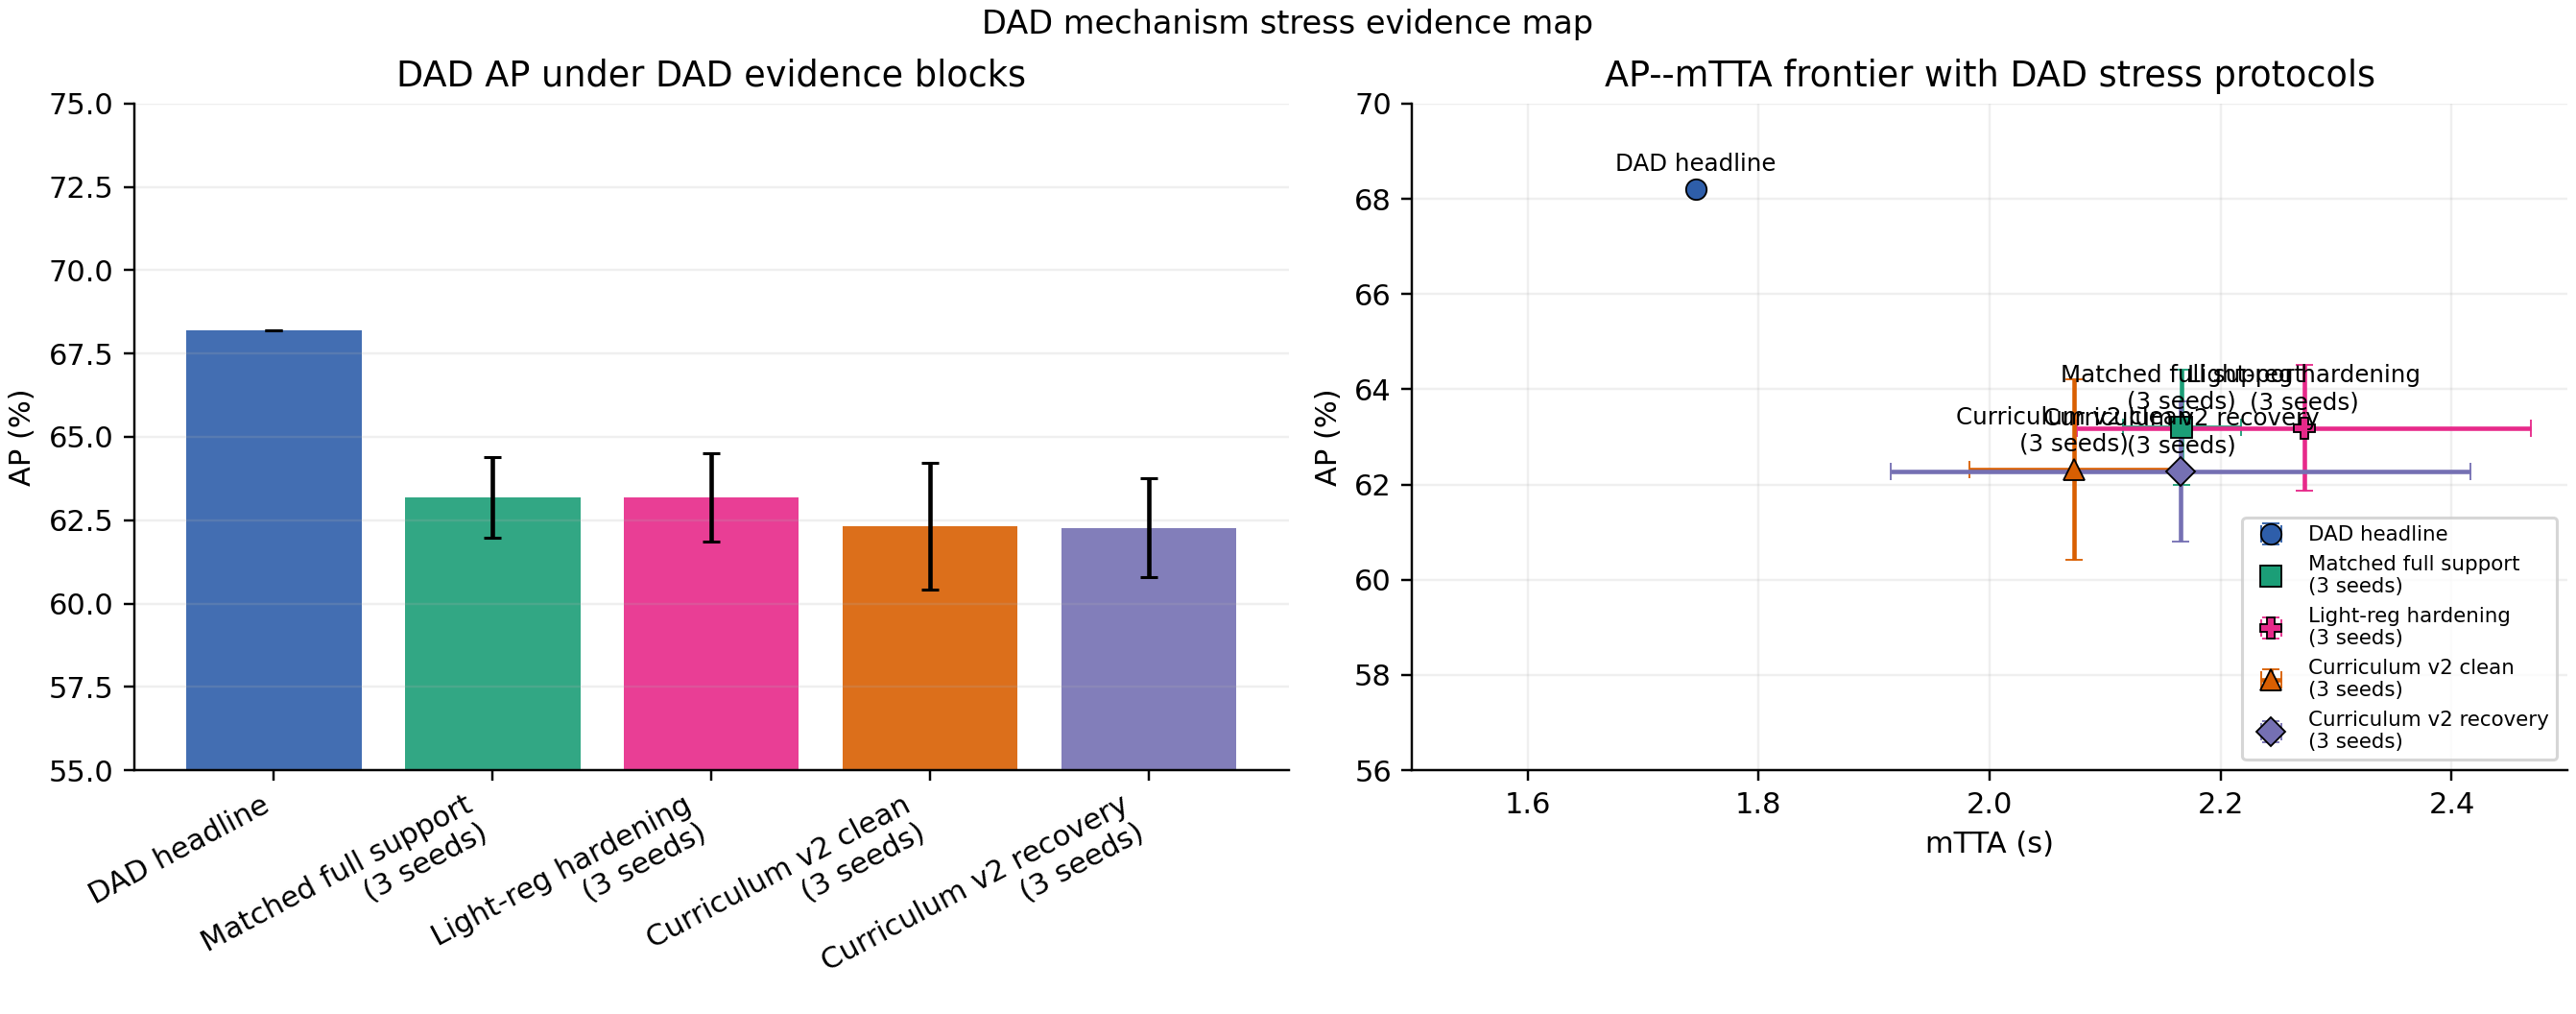
\includegraphics[width=0.98\textwidth]{../figures/insight_fig6_dad_stress_summary.pdf}
\caption{[Mechanism stress evidence] DAD mechanism-stress evidence across protocol blocks. We report three
support tiers against the canonical headline run: matched full-support,
light-regularization hardening, and curriculum-recovery expansion. Error bars
mark seed-level mean and standard deviation on AP and mTTA so the stress-story is
read as a frontier band rather than a single favorable point.}
\label{fig:dad_stress_summary}
\end{figure*}

\subsection{Main Predictive Results on A3D}

\begin{table}[t]
\caption{[Headline evidence] A3D results. \method{} reaches a strong
interpretable operating point
with better warning lead time than CRASH while maintaining competitive AP.}
\label{tab:a3d}
\centering\small
\setlength{\tabcolsep}{3pt}
\resizebox{\linewidth}{!}{%
\begin{tabular}{lccccc}
\toprule
Method & AP$\uparrow$ & mTTA$\uparrow$ & TTA@R80$\uparrow$ & P@R80$\uparrow$ & Interface\\
\midrule
CRASH~\citep{liao2024crash} & 96.0\% & 4.27s & -- & -- & none\\
W3AL~\citep{liao2024and}    & 92.4\% & 4.52s & -- & -- & verbal\\
\midrule
\method{} & 93.4\% & 4.90s & 4.89s & 0.9067 & semantic\\
$\Delta$ vs.\ CRASH & $-2.60\%$ & $+14.8\%$ & -- & -- & --\\
\bottomrule
\end{tabular}%
}
\end{table}

On A3D, \method{} achieves a stronger and cleaner paper-facing result. The
model improves mTTA over CRASH while maintaining competitive AP, which places
it in a favorable interpretable region of the accuracy--timeliness plane.
Because A3D offers more progressive hazard development than DAD, it also serves
as the dataset where the semantic-interface story is easiest to read:
conceptual precursors appear early enough to support both prediction and
auditing.

\paragraph{A3D headline stability.}
The flagship A3D recipe also remains stable across three seeds. A dedicated
headline audit yields $\text{AP}=94.16\%\pm0.95$ and
$\text{mTTA}=4.62\pm0.42$~s, which matters because A3D is the paper's cleanest
semantic-interface dataset. This multi-seed result does not change the main
claim, but it makes the strongest table in the paper materially more stable
under scrutiny.

\begin{figure*}[t]
\centering
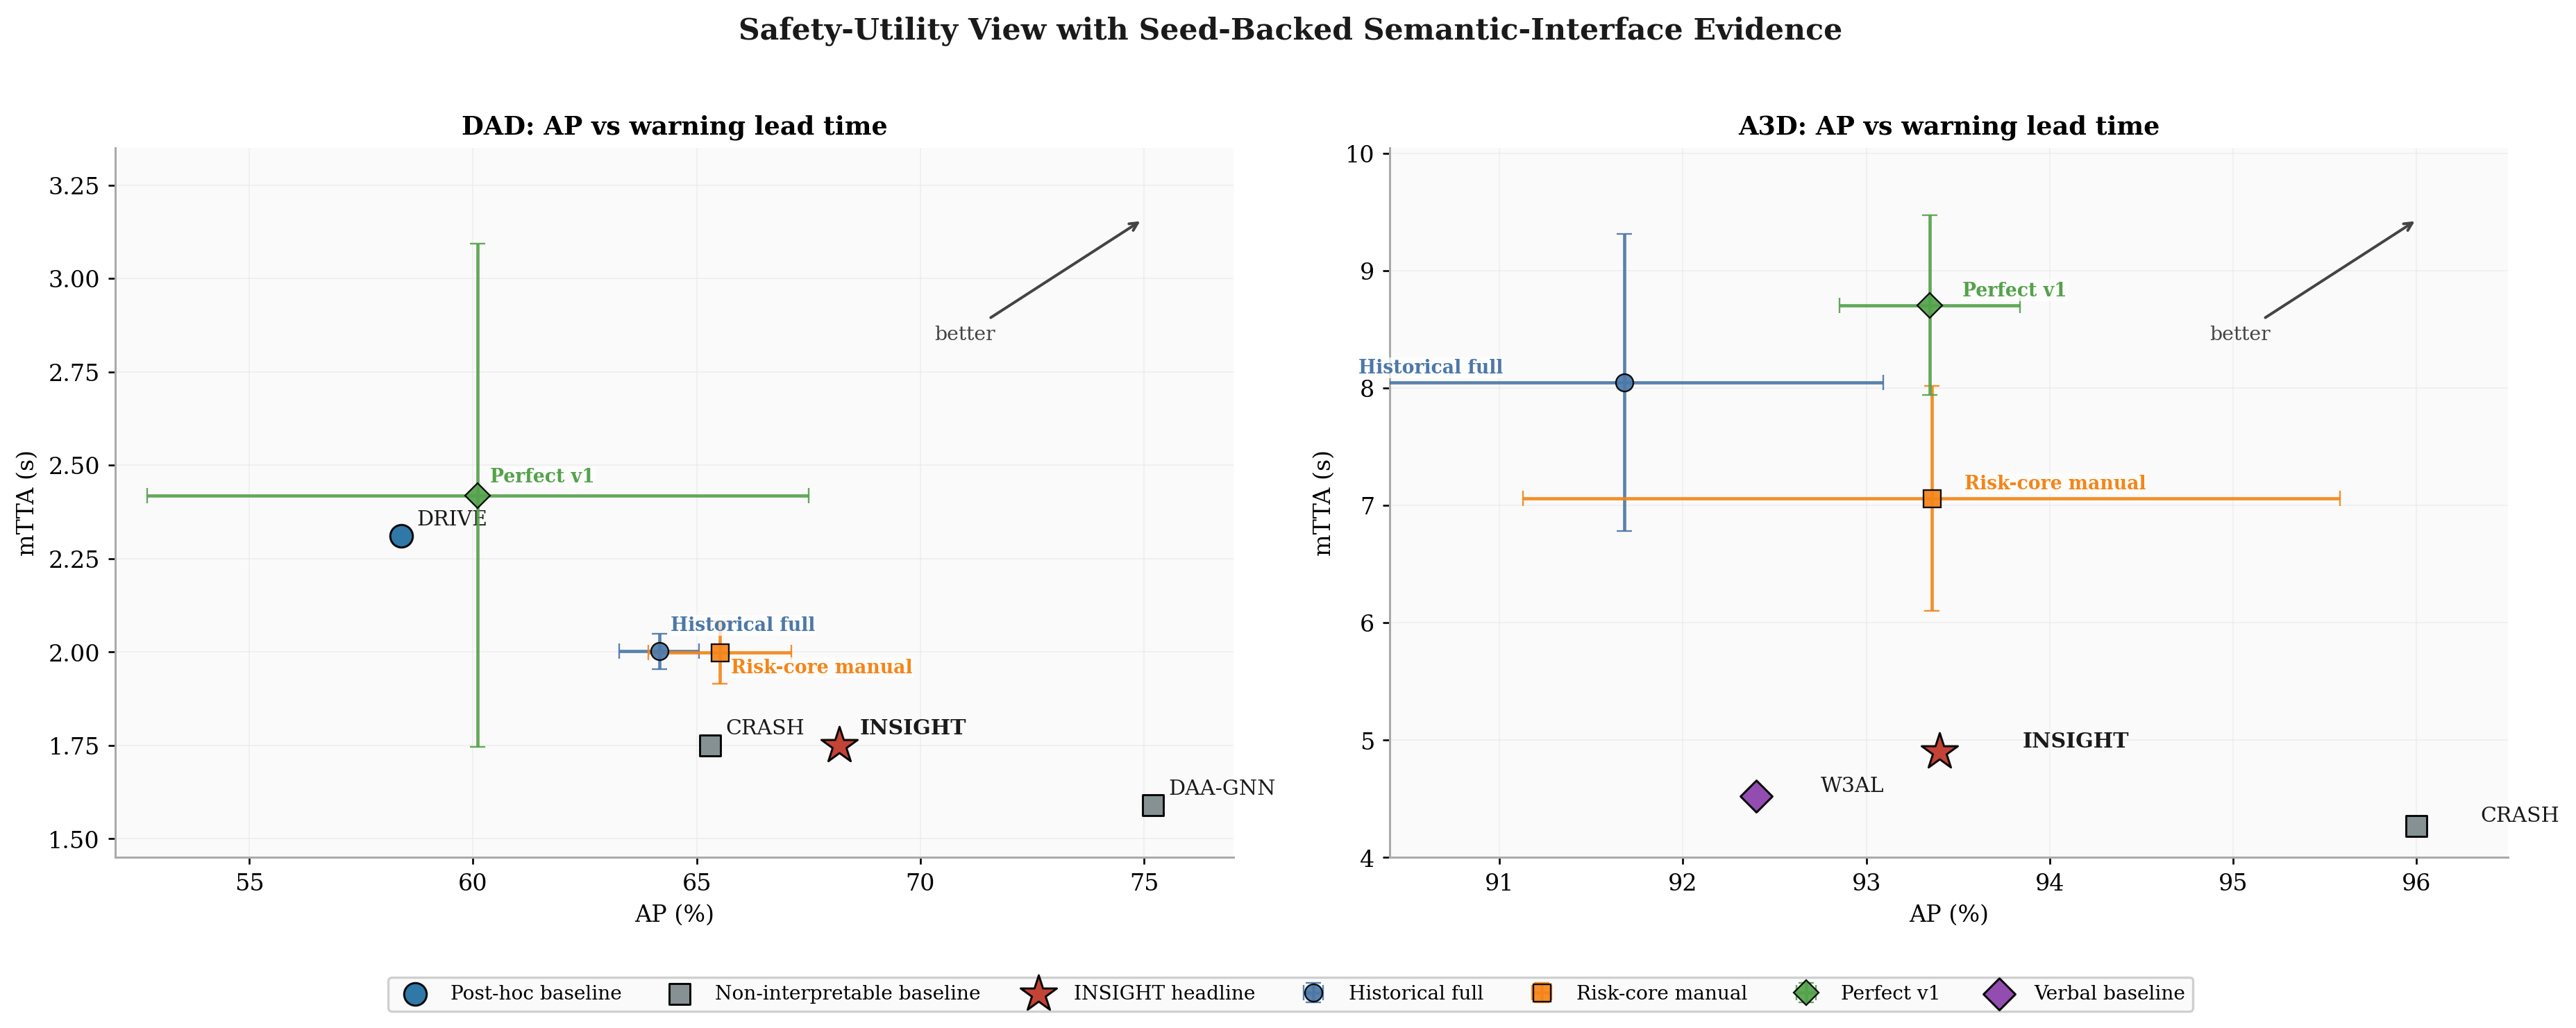
\includegraphics[width=0.98\textwidth]{../figures/insight_fig5_safety_utility.pdf}
\caption{[Reading bridge: headline + controlled support] Safety--utility view under semantic-interface constraints. Literature
baselines and headline \method{} points are shown as table values, while the
colored ontology markers show three-seed matched-launcher aggregates with
horizontal AP and vertical mTTA standard-deviation intervals. The figure makes
the evidence tiers explicit: \method{} occupies a competitive interpretable
operating point, and ontology choice measurably moves the AP--mTTA frontier.}
\label{fig:safety_utility}
\end{figure*}

Figure~\ref{fig:safety_utility} complements the tables by making the paper's
position explicit: the target operating regime is strong anticipation with an
auditable semantic layer.

\subsection{Ontology Choice Changes the Operating Point}

\begin{table*}[t]
\caption{[Controlled support evidence] Matched ontology comparison under the
shared launcher protocol. Only
the ontology source varies; the training launcher family is held fixed.}
\label{tab:concept_sets}
\centering\small
\begin{tabular}{llccccc}
\toprule
Dataset & Concept set & \#Concepts & AP$\uparrow$ & mTTA$\uparrow$ & TTA@R80$\uparrow$ & P@R80$\uparrow$\\
\midrule
DAD & Historical full & 837 & 64.91\% & 1.88s & 2.51s & 0.492 \\
DAD & Risk-core manual & 30 & \textbf{65.25\%} & 2.15s & \textbf{2.92s} & 0.462 \\
DAD & Perfect concept set v1 & 80 & 64.15\% & \textbf{2.30s} & 2.67s & 0.467 \\
\midrule
A3D & Historical full & 837 & 93.88\% & 9.41s & 8.13s & 0.940 \\
A3D & Risk-core manual & 30 & 94.36\% & \textbf{9.57s} & \textbf{8.60s} & \textbf{0.944} \\
A3D & Perfect concept set v1 & 80 & \textbf{96.54\%} & 8.69s & 7.11s & 0.934 \\
\bottomrule
\end{tabular}
\end{table*}

Table~\ref{tab:concept_sets} is one of the most important result blocks in the
paper. It shows that ontology choice changes the AP--mTTA frontier rather than
yielding one universally dominant vocabulary. On DAD, the compact manual set
has the highest AP under the shared recipe, while the polished discovered
ontology gives the best mTTA. On A3D, the discovered ontology achieves the
strongest AP, while the compact manual set gives the best timing metrics. The
scientific lesson is that ontology design is not decoration: it is an
experimental variable that changes downstream behavior. This is the paper's
most direct evidence that language-side design decisions survive contact with
model training: changing canonical names, merge policy, and family structure at
the ontology level changes the downstream operating point under one matched
launcher family.

This claim is now backed by a complete three-seed extension over all six
dataset--ontology cells. Across the matched ontology block, all $18/18$
recommended seeded runs are finished. On A3D, the paper-facing discovered
ontology remains competitive under this aggregate view
($93.35\%\pm0.49$ AP, $8.71\pm0.77$~s mTTA), so the ontology effect is not
resting on one favorable seed. On DAD, however, the discovered ontology shows
substantially larger variance ($60.11\%\pm7.40$ AP), which is exactly why we
continue to describe DAD as the fragile side of the paper rather than trying
to oversell a uniform robustness story.

\subsection{Current Timing and Intervention Evidence}

\begin{table}[t]
\caption{[Mechanism stress evidence] Matched score-source comparison on
representative checkpoints. The
same trained checkpoint is evaluated twice: once with the classifier score
trajectory and once with the actor policy score trajectory. These are support
analyses, not canonical headline results.}
\label{tab:trigger_compare}
\centering\small
\setlength{\tabcolsep}{3pt}
\resizebox{\linewidth}{!}{%
\begin{tabular}{llcccc}
\toprule
Dataset & Score source & AP$\uparrow$ & mTTA$\uparrow$ & TTA@R80$\uparrow$ & P@R80$\uparrow$\\
\midrule
DAD & classifier & 61.94\% & 2.16s & 2.87s & 0.486 \\
DAD & actor & 34.67\% & 2.08s & 5.00s & 0.349 \\
\midrule
A3D & classifier & 93.88\% & 4.71s & 4.06s & 0.940 \\
A3D & actor & 91.14\% & 4.97s & 4.94s & 0.911 \\
\bottomrule
\end{tabular}%
}
\end{table}

Table~\ref{tab:trigger_compare} clarifies the scope of the timing claim. On
A3D, actor-based evaluation is fairly close to the classifier line on a
representative checkpoint, suggesting that concept-conditioned timing is
plausible beyond the classifier trajectory. On DAD, actor-based evaluation is
still substantially weaker, which is why the paper continues to report
classifier-derived headline metrics. This is precisely why we do not let the
actor branch carry the main paper claim. This comparison therefore works best
as a transfer test: it shows how much timing behavior survives when we switch
from the classifier trajectory to the learned actor policy.

An extended DAD trigger-source audit over six same-family support checkpoints
reinforces this cautious reading rather than weakening it. Across that block,
classifier-based evaluation averages $61.11\%\pm4.58$ AP and
$2.17\pm0.19$~s mTTA, whereas actor-based evaluation averages
$37.41\%\pm7.35$ AP and $3.73\pm1.39$~s mTTA. The actor's threshold-crossing
rate is also unstable across checkpoints, which means the current policy
branch should still be read as partial timing evidence rather than as a mature
replacement for classifier-derived anticipation scores.

Archived prediction-timing analyses nevertheless provide useful support for the
semantic interface story. The classifier branch crosses threshold before impact
on many positive cases, and archived concept amplification experiments show that
positive concept edits can move alerts earlier on a non-trivial subset of
valid edited cases. Together, these results show that the interface is
structurally meaningful and partially intervenable, while a complete
policy-level causal timing account lies beyond the current paper.

\subsection{Ontology Quality as Evidence, Not Decoration}

The ontology work is not merely qualitative preprocessing. The paper-facing
artifacts record a source pool of more than 600 candidate phrases, an
order-of-magnitude compression to a paper-ready ontology of about 80 concepts,
family-balance audits across nine semantic families, canonical merge examples,
and light human review notes. The point of these assets is scientific
accountability: if ontology construction is part of the method, then the
ontology itself should be inspectable, comparable, and citable as evidence.
This is one of the main differences between our approach and systems that
inherit their semantic vocabularies implicitly. For EMNLP, this evidence block
is central: the contribution is not only that the model has concepts, but that
the exposed semantic layer is named, canonicalized, reviewable, and tied to
explicit provenance.

Concretely, the paper-facing audit trail compresses 611 mined phrases into a
post-polish pool of 81 canonical candidates and a finalized release of 80
reviewed concepts. The retained vocabulary is distributed across nine explicit
families, and the current human-review log covers all 80 retained concepts with
light-touch keep decisions rather than ontology rebuilding. We view this as an
important distinction: the paper is not claiming a finished lexical resource,
but a governed semantic interface whose canonical names, family coverage, and
merge provenance can be inspected directly.

\begin{figure}[t]
\centering
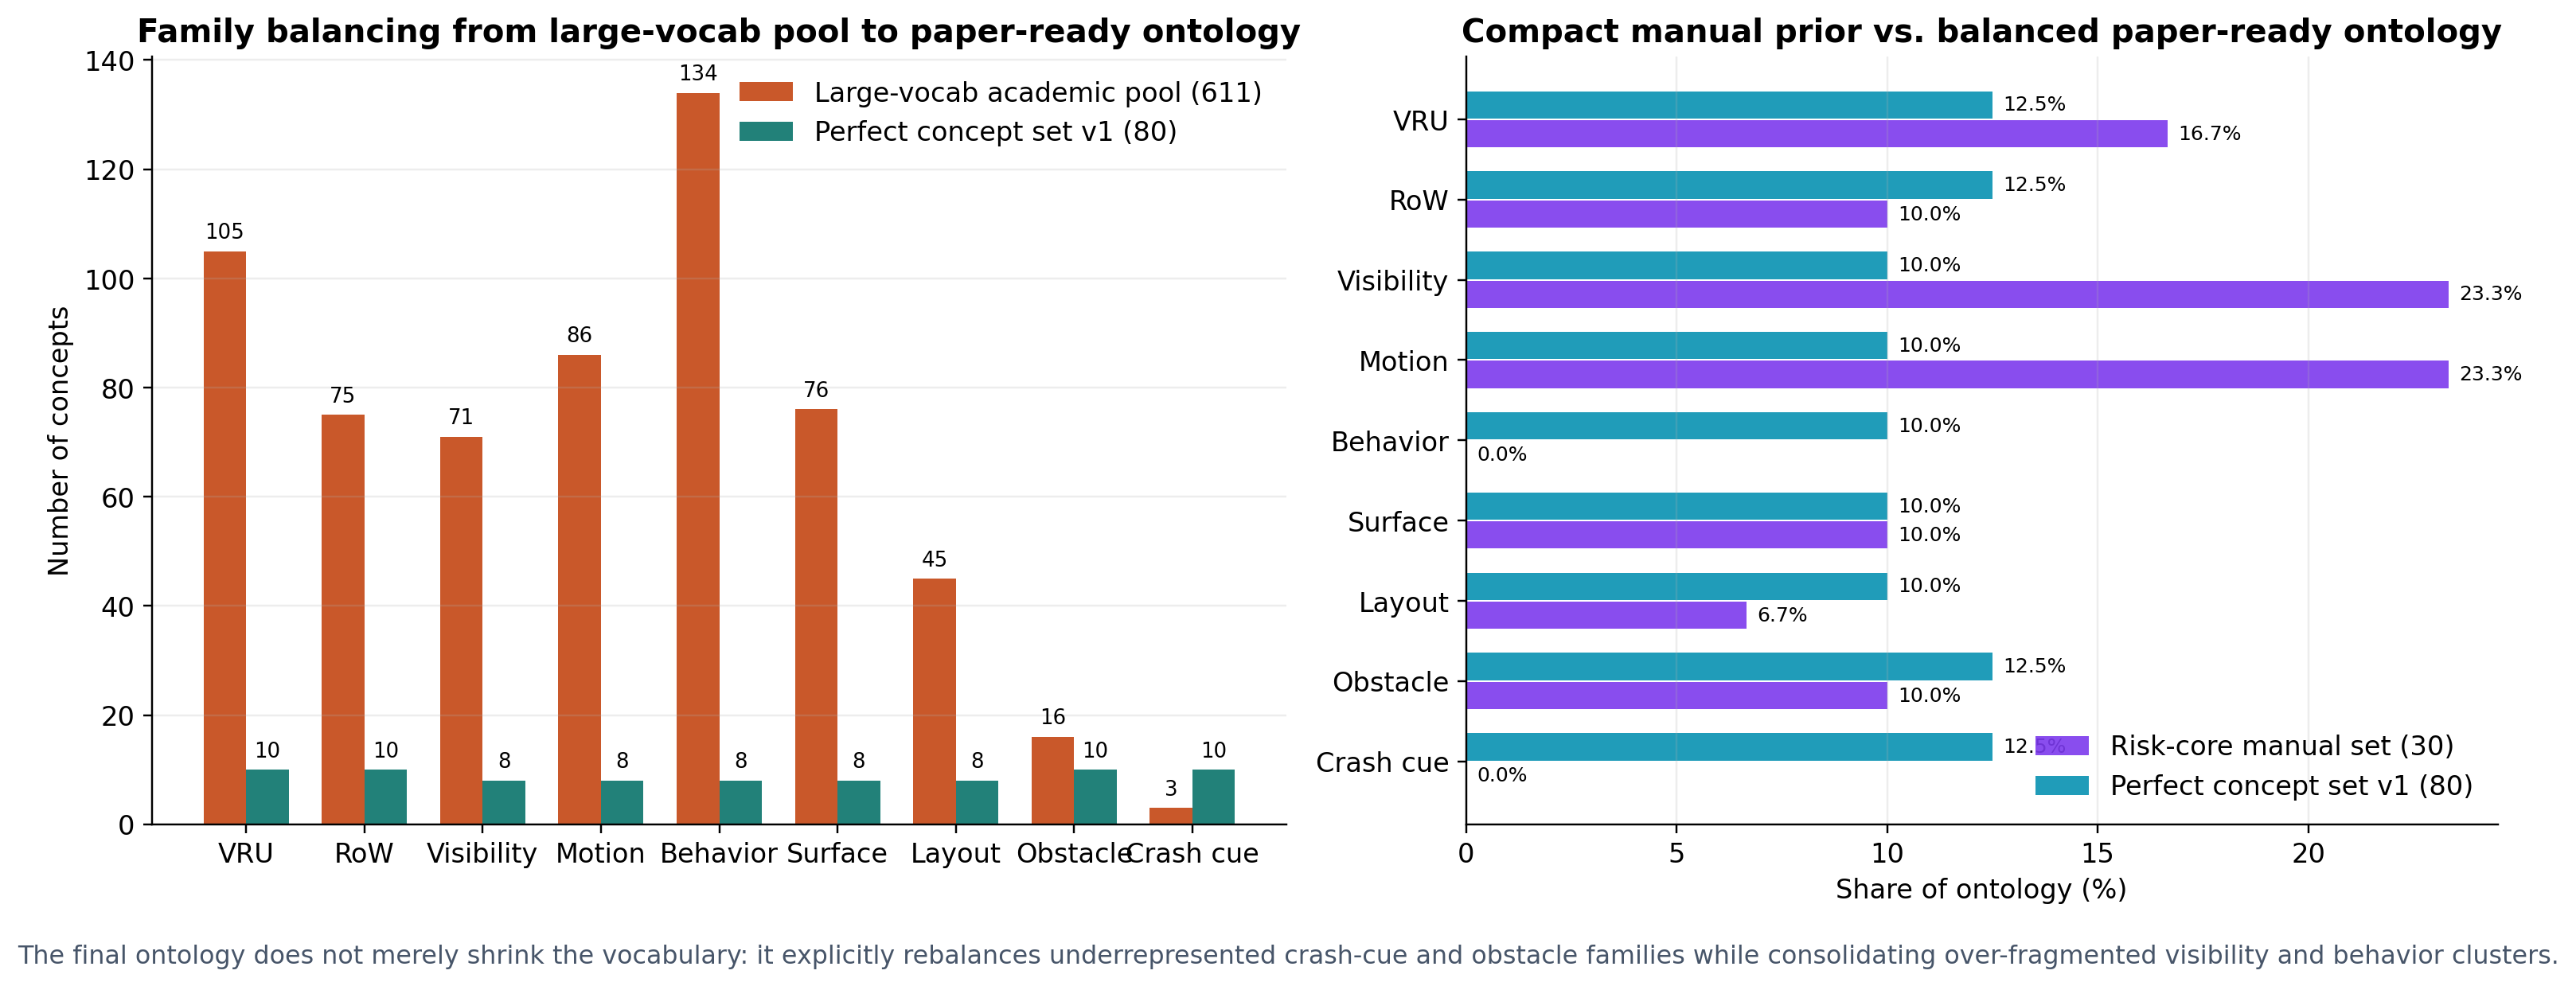
\includegraphics[width=0.98\linewidth]{../figures/insight_fig_concept_family_coverage.pdf}
\caption{[Language-side support evidence] Family coverage in the paper-facing ontology. The polished concept
set deliberately redistributes capacity toward accident-relevant semantic
families, making the ontology easier to audit and more aligned with the target
task than a broad ungoverned phrase pool.}
\label{fig:ontology_family_main}
\end{figure}

\begin{figure*}[t]
\centering
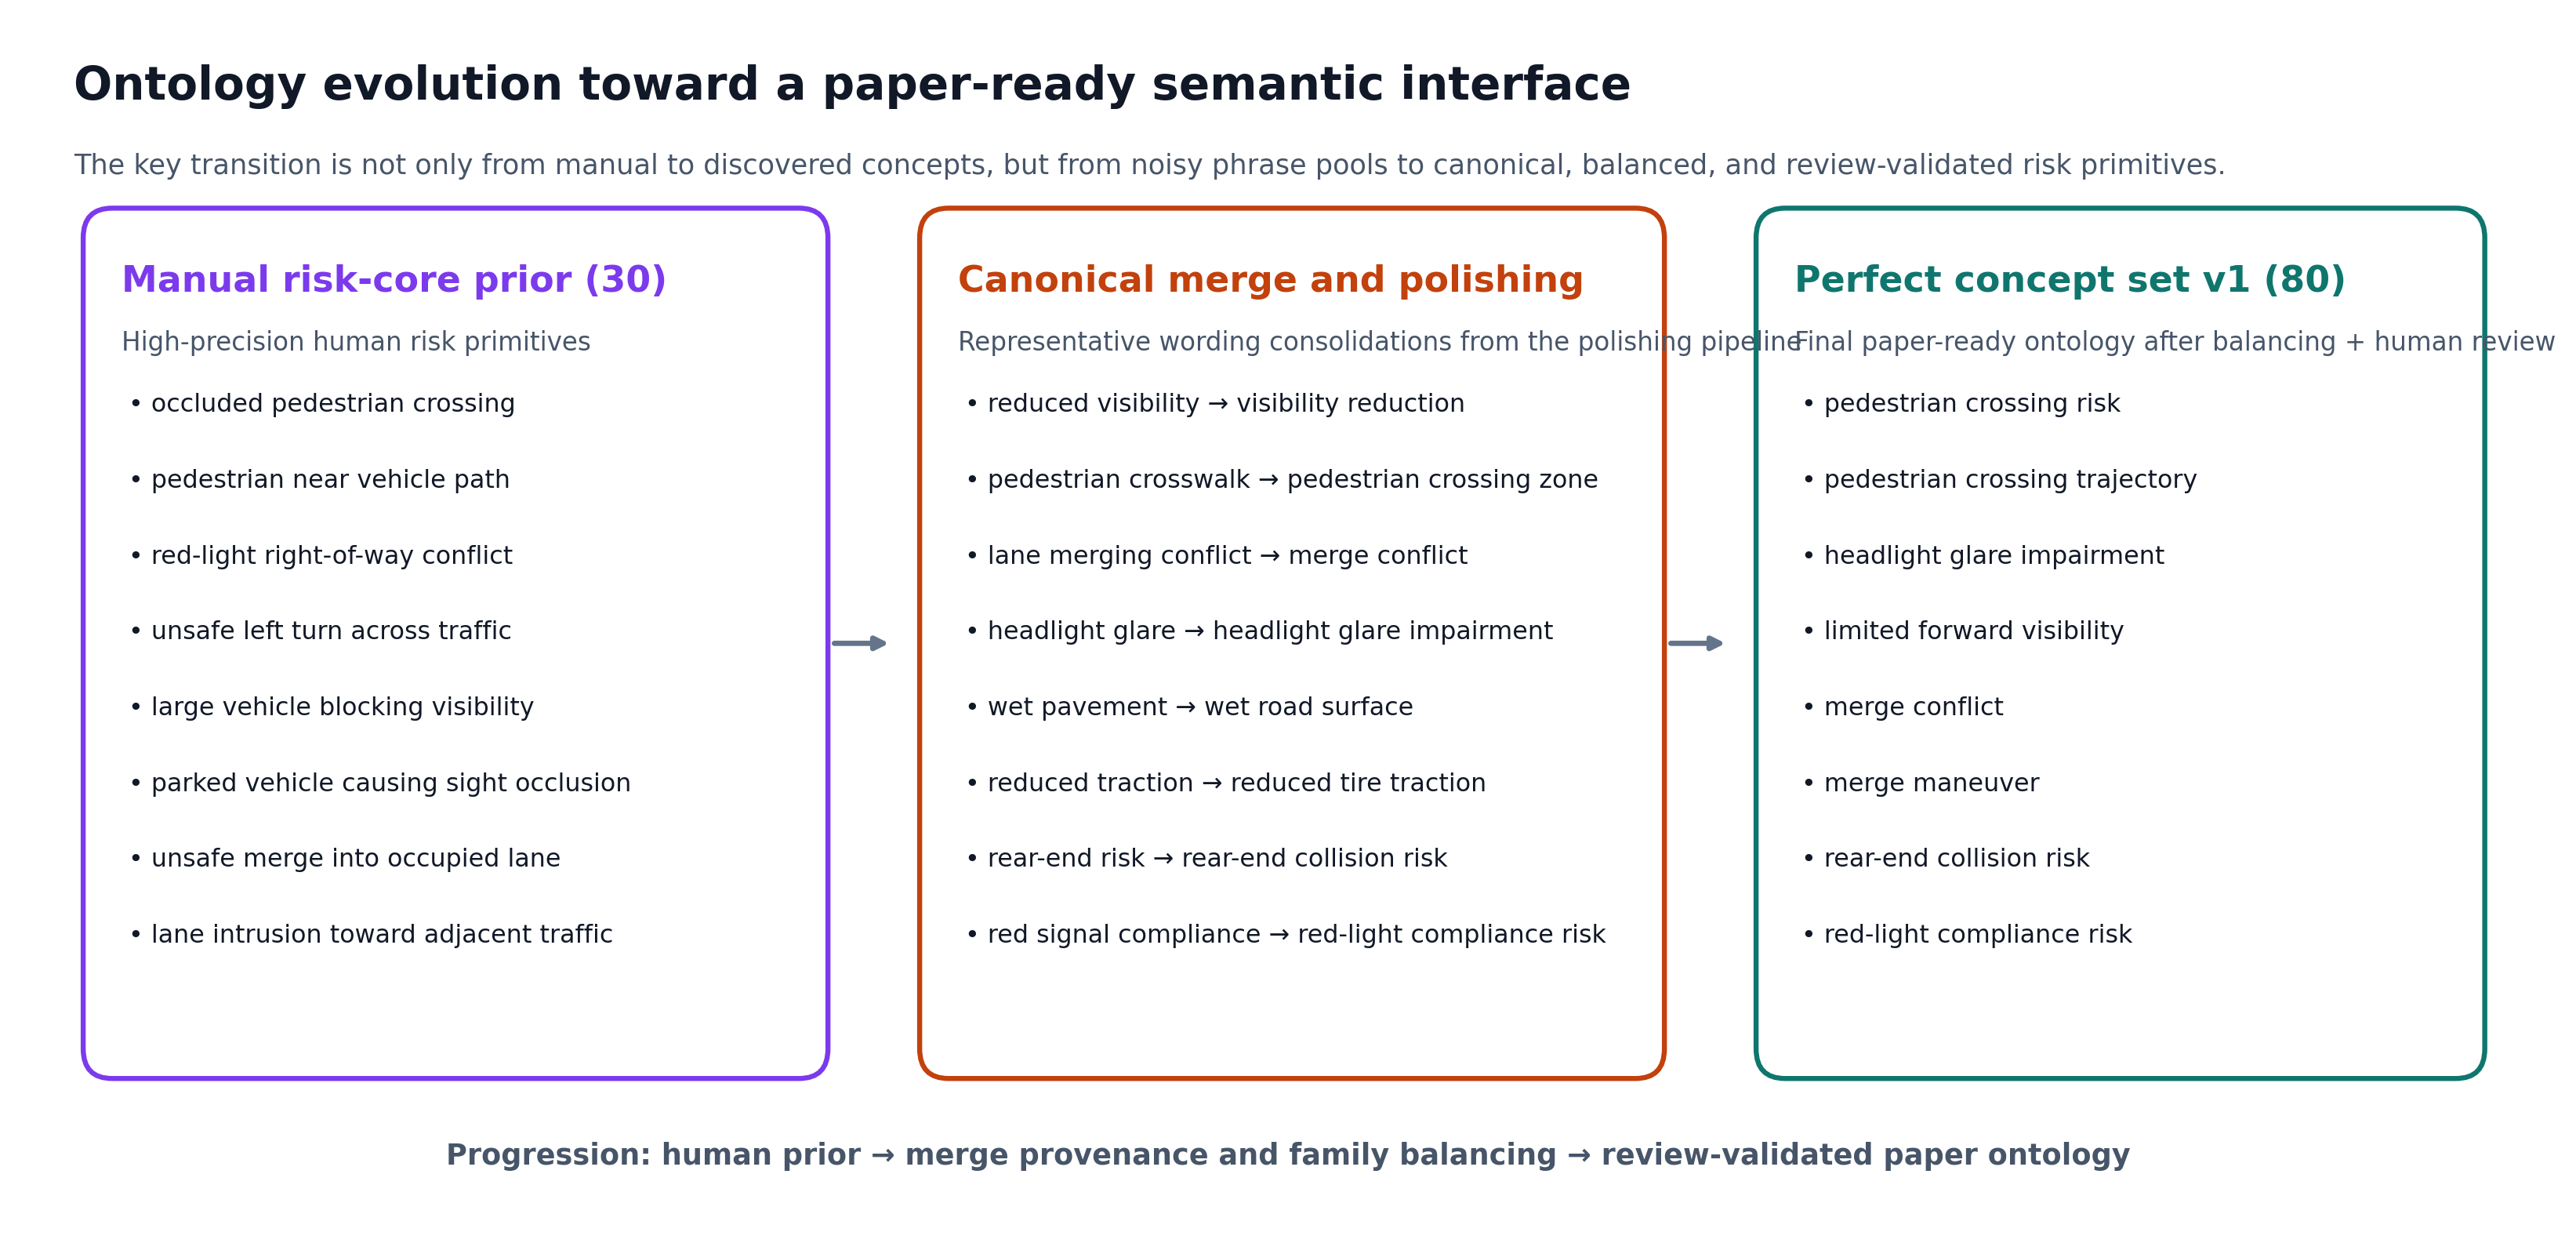
\includegraphics[width=0.98\textwidth]{../figures/insight_fig_concept_evolution.pdf}
\caption{[Language-side support evidence] Ontology evolution toward a paper-ready semantic interface. The
semantic bottleneck is not fixed once and for all: we start from a compact
human prior, consolidate noisy large-vocabulary proposals through canonical
merge and family balancing, and then finalize a reviewed ontology that can be
used consistently in both experiments and paper-facing audits.}
\label{fig:ontology_evolution_main}
\end{figure*}

Figures~\ref{fig:ontology_family_main} and
\ref{fig:ontology_evolution_main} illustrate the kind of evidence we want the
ontology to provide: not only a list of names, but a task-facing semantic
structure whose coverage, merge provenance, and review trajectory can be
inspected quantitatively. This is why ontology design appears as a scientific
variable in Table~\ref{tab:concept_sets} rather than as a hidden prompt choice.

\subsection{Concept-Level Quantitative Evidence}

\begin{table}[t]
\caption{[Mechanism stress evidence] Quantitative semantic-interface
diagnostics from archived DAD
analyses. These diagnostics complement the case studies by quantifying timing
alignment, edit sensitivity, and actor behavior in the archived DAD assets.}
\label{tab:interp_quant}
\centering\scriptsize
\setlength{\tabcolsep}{2.5pt}
\resizebox{\linewidth}{!}{%
\begin{tabular}{p{0.23\linewidth}p{0.14\linewidth}p{0.25\linewidth}p{0.30\linewidth}}
\toprule
Diagnostic & Samples & Main statistic & Reading \\
\midrule
Prediction timing & 39 valid positives & mean lead = 39.41 frames ($\approx$1.97s) & event-aligned timing is measurable before impact \\
Hybrid amplification & 50 edited cases & mean shift = $-2.04$ frames & positive edits can advance alerts in some cases \\
Hybrid amplification & 50 edited cases & earlier / same / later = 14\% / 84\% / 2\% & edit effects are heterogeneous, not universal \\
Zero-baseline edit & 25 edited cases & mean shift = 0.00 frames & null-style edit has no systematic timing effect \\
Top-risk edit & 25 edited cases & mean shift = 0.00 frames & naive top-risk edits alone do not guarantee movement \\
Actor diagnostic & 48 cases & mean actor peak = 0.498 & archived actor outputs are too flat for strong policy claims \\
\bottomrule
\end{tabular}%
}
\end{table}

Table~\ref{tab:interp_quant} records what the archived analyses support
quantitatively: prediction timing can be aligned
to accident onset, positive concept edits can move alerts earlier on a
meaningful subset of cases, and the archived actor branch is too flat for
strong policy claims. These numbers support the paper's current stance: the
semantic interface is architecturally transparent and partially audited, but it
is not yet a finished human-verified concept benchmark or a complete causal
timing proof. That asymmetry is intentional in our presentation: the paper is
strongest as a semantic-interface paper, not as a claim that every downstream
timing component is already equally mature.

\subsection{Ablation and Efficiency}

\begin{table}[t]
\caption{[Controlled support evidence] Component ablation on DAD under a
controlled support protocol. These runs are not the canonical headline
line; their purpose is to
isolate how much the concept interface and its support modules matter under a
shared recipe.}
\label{tab:ablation}
\centering\small
\setlength{\tabcolsep}{4pt}
\resizebox{\linewidth}{!}{%
\begin{tabular}{lccc}
\toprule
Variant & AP$\uparrow$ & mTTA$\uparrow$ & TTA@R80$\uparrow$\\
\midrule
Full \method                  & \textbf{68.84\%} & \textbf{2.42s} & \textbf{3.15s}\\
\quad w/o \caac{} (CBM-only)  & 67.1\% & 1.75s & 2.31s\\
\quad w/o \cgta{}             & 67.8\% & 2.19s & 2.87s\\
\quad w/o \crs{}              & 68.2\% & 2.31s & 3.02s\\
\quad w/o \tsd{}              & 67.5\% & 2.28s & 2.95s\\
\quad w/o \cbm{} (no concepts)& 65.3\% & 1.82s & 2.44s\\
\bottomrule
\end{tabular}%
}
\end{table}

The ablation shows that the semantic interface participates in predictive
behavior, but the DAD mechanism story should still be read with some care and as
mechanism-support rather than headline evidence. Within this controlled support
line, removing the concept bottleneck hurts performance, and removing the
timing consumer or concept-linked temporal modeling also weakens the operating
point. At the same time, our broader three-seed support family for DAD ablations
shows that the no-\cbm{} variant can remain competitive on AP under some matched
support recipes. We therefore avoid the stronger claim that DAD gains are
explained by the concept bottleneck alone. The safer reading is that the
semantic interface, temporal coupling, and training recipe interact, with A3D
providing the cleaner mechanism story and DAD providing the more fragile one.

Archived A3D support ablations point in the same direction but with a cleaner
mechanism profile. In that family, removing the concept bottleneck lowers AP
from $94.75\%$ to $93.47\%$ and mTTA from $4.81$~s to $4.61$~s, while removing
reconstruction lowers AP to $93.38\%$. Removing alignment raises AP to
$96.03\%$, but it simultaneously shortens mTTA to $4.27$~s and TTA@R80 to
$3.70$~s from the full line's $4.44$~s. We therefore read A3D as evidence that
the semantic interface is most convincing as an operating-point design: some
auxiliary terms can trade AP against timing, but removing the bottleneck itself
still weakens the cleaner paper-facing support family.

From an efficiency perspective, \method{} remains in a small-model regime
(about 30M parameters), far below several strong but non-interpretable
alternatives. The practical claim is therefore modest but relevant:
architectural auditability does not require the largest models in the current
literature.

\paragraph{Cross-dataset interpretation.}
Taken together, the results suggest that \method{} is strongest when hazards
develop progressively enough for semantic precursor cues to appear before
impact. This likely explains the stronger A3D behavior. DAD still benefits,
but offers a narrower and noisier early-warning window, so claims there are
fragile support rather than a settled high-confidence mechanism statement.

\subsection{Qualitative Interface Evidence}

\begin{figure*}[t]
  \centering
  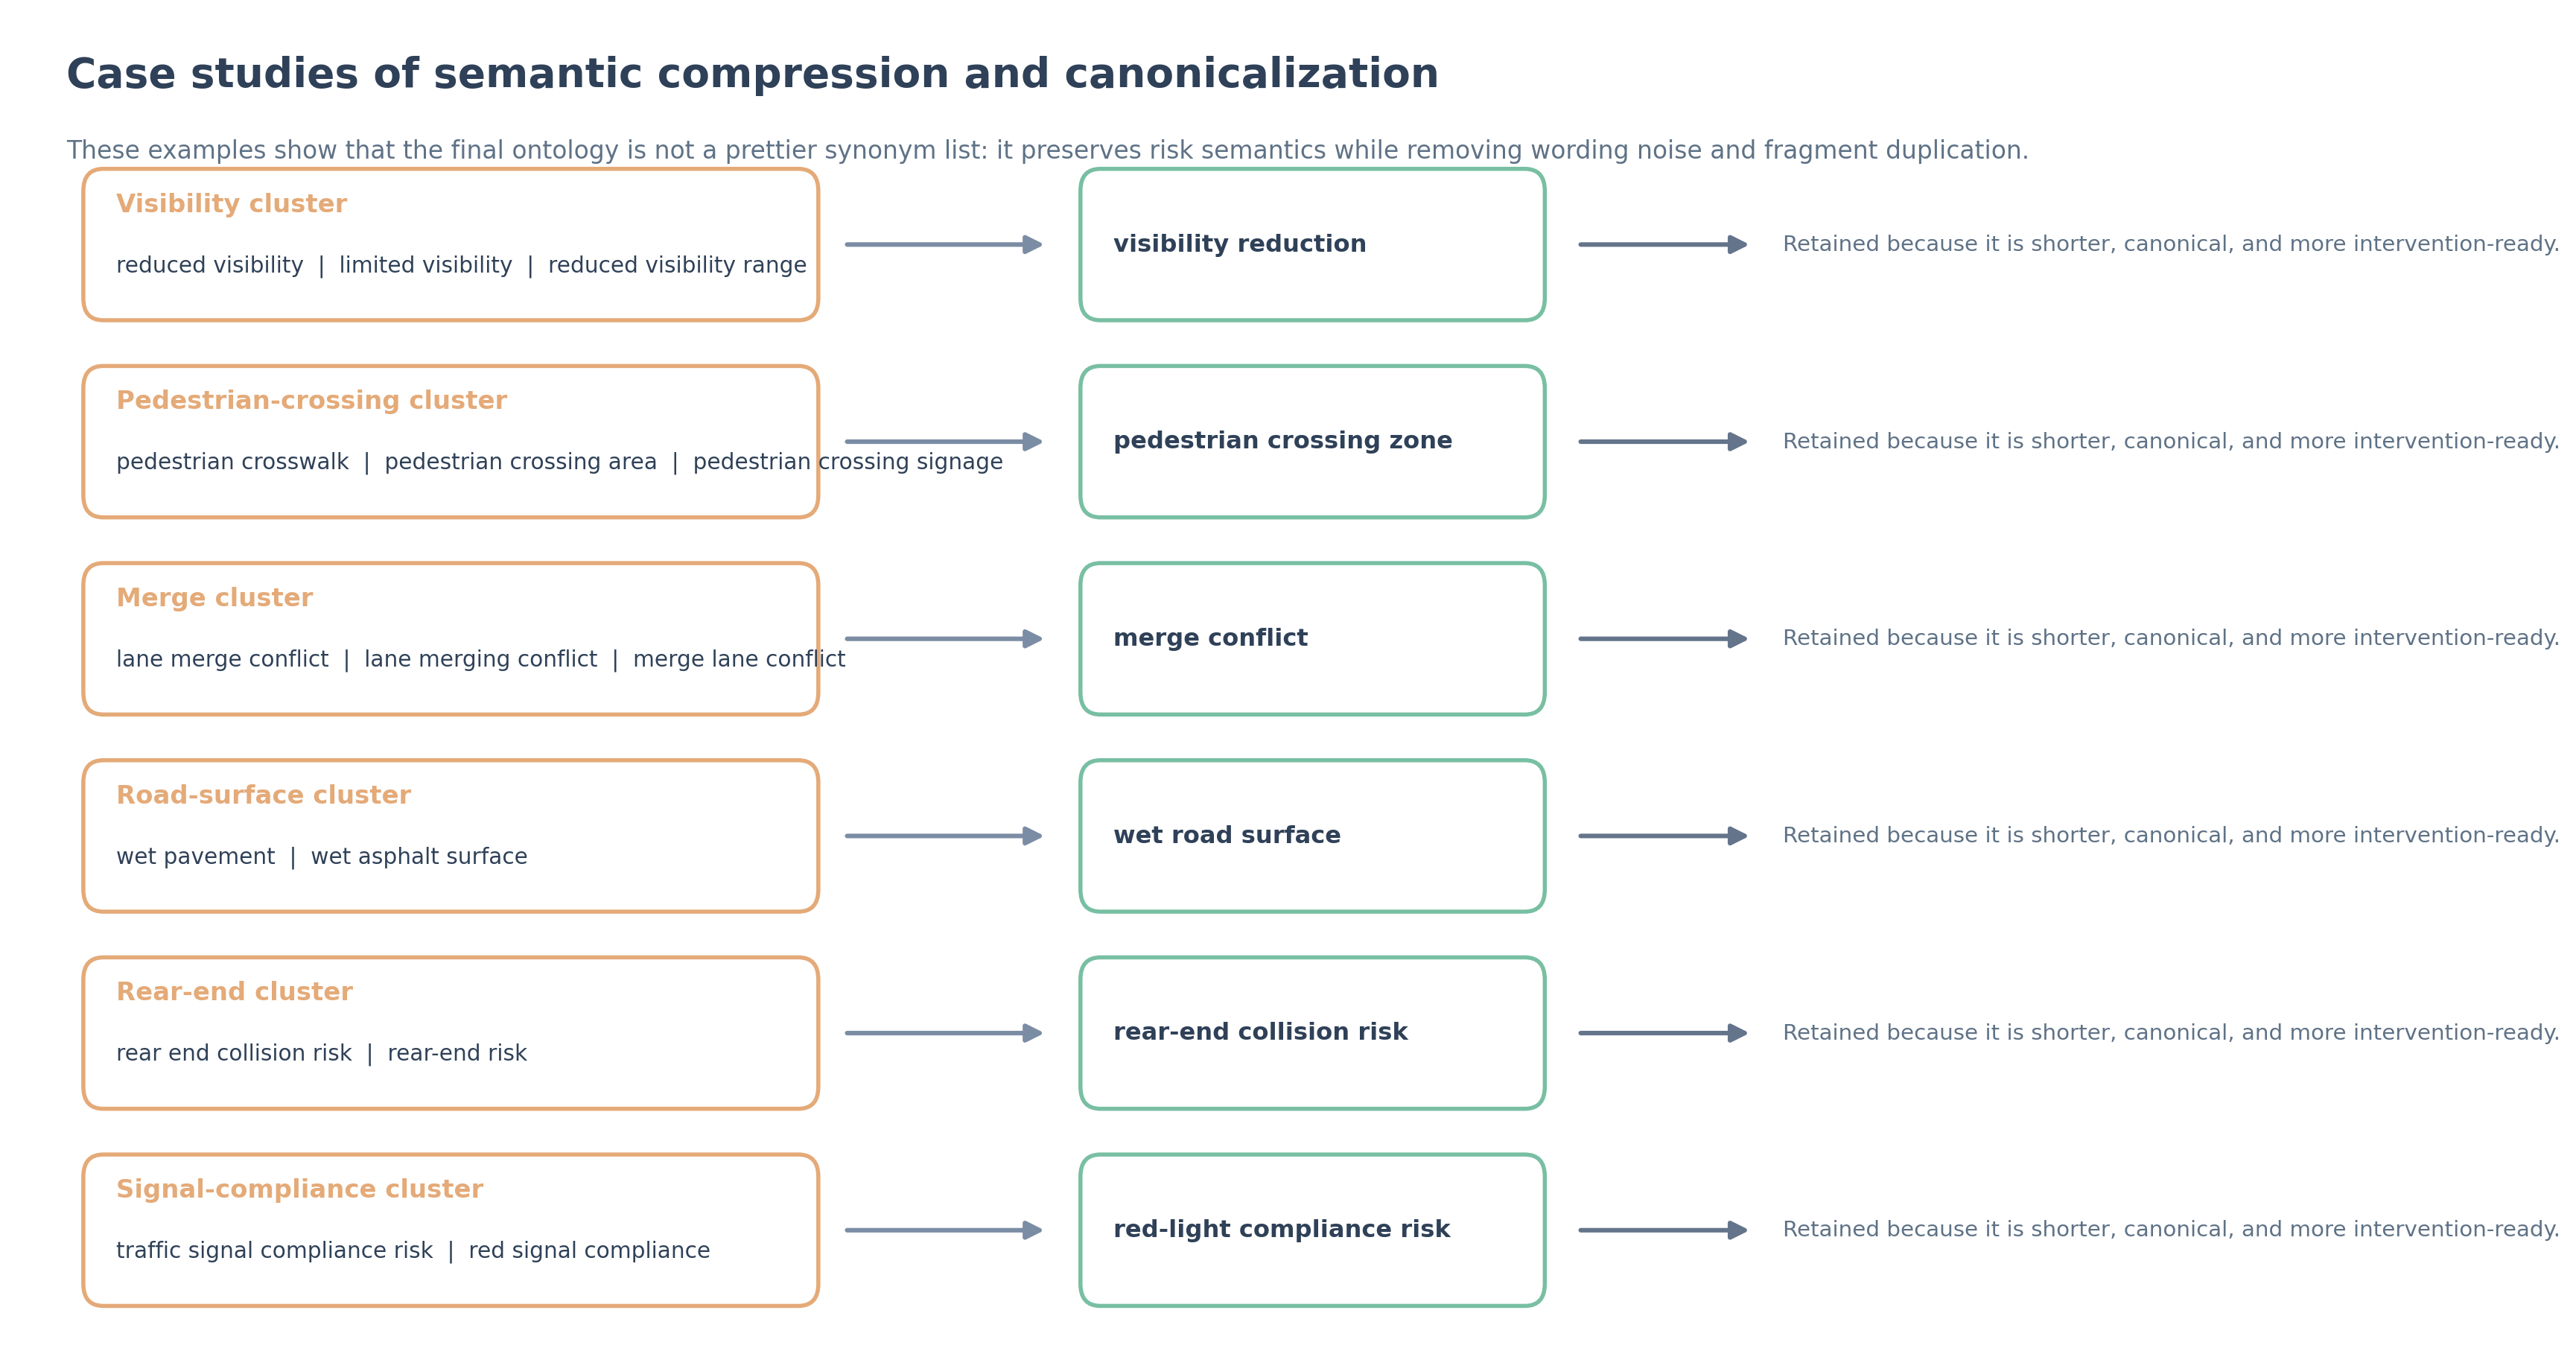
\includegraphics[width=0.985\textwidth]{../figures/insight_fig_concept_case_study.pdf}
  \caption{\textbf{Canonical merge examples from the paper-facing ontology.}
  The final ontology is not just shorter than the raw proposal pool. It
  preserves risk semantics while consolidating wording noise into canonical,
  intervention-ready concepts such as \emph{visibility reduction},
  \emph{pedestrian crossing zone}, and \emph{merge conflict}.}
  \label{fig:concept_case_study_main}
\end{figure*}

Figure~\ref{fig:motivation} already shows the semantic interface in use on a
real crash case, where concept activations and temporal evolution can be read
directly against the scene progression. Figure~\ref{fig:concept_case_study_main}
complements that example from the ontology side by making the canonical merge
policy concrete. Together, these figures show what we mean by a paper-ready
semantic interface: readable at inference time, but also governed as a stable
research artifact rather than as an ad hoc phrase bank.

\section{Conclusion}
\label{sec:conclusion}

We presented \method{}, a framework built around a language-grounded risk
concept interface for accident anticipation. The central contribution of the
paper is to show that such an interface can be constructed explicitly and
studied as a scientific object. In our setting, that means treating ontology
construction as part of the method rather than as hidden preprocessing, then
training an interpretable anticipation model on top of the resulting ontology.

This shift in perspective changes what the paper contributes. First, we provide
a reproducible pipeline for mining, refining, merging, balancing, and lightly
reviewing risk concepts from driving frames. Second, we show that the resulting
ontology is not merely descriptive: when deployed as the concept bottleneck of
the model, ontology choice changes the AP--mTTA operating point under matched
launchers. Third, we show that strong anticipation can coexist with a compact
and auditable semantic layer, including a competitive interpretable tier on DAD
and cleaner timing behavior on A3D.

Empirically, the paper is strongest on the semantic layer: the ontology
pipeline, the concept bottleneck, the controlled ontology comparisons, and the
case-study and audit artifacts. The timing module remains important as the
downstream consumer of semantic state, but the paper should be read first as a
semantic-interface contribution and only second as a policy-timing paper. The
actor-policy results are therefore useful mainly insofar as they clarify how
much of that behavior transfers beyond the classifier trajectory.

\paragraph{Limitations and future work.}
The concept labels are still based on CLIP-style pseudo-annotations rather than
human-verified frame-level concept supervision. The current semantic interface
is therefore auditable and trainable, but not yet a finished concept benchmark.
The evaluation also relies on offline visual features rather than end-to-end
video backbones. More importantly, while the timing module consumes the concept
state by construction, a complete policy-level intervention validation study
remains future work. We have strengthened the language-facing evidence with a
larger frame audit and full light-touch review of the released ontology, so the
main remaining empirical weakness is no longer missing ontology coverage but
DAD-side instability, limited cross-dataset ontology transfer evidence, and the
gap between classifier-derived anticipation scores and mature policy-level
timing behavior.

\paragraph{Evidence scope.}
To keep methodological integrity, the paper explicitly treats DAD as a
stress setting, not a universal performance frontier, and treats actor-policy
timing as a partial, support-only account. This choice keeps the central claim
on the part of the evidence that is strongest: concept-interface construction,
matched protocol contrast, and clean A3D flagship stability.

\paragraph{Broader impact.}
For safety-critical prediction, the practical value of \method{} is not merely
that it forecasts accidents, but that it exposes a more inspectable semantic
state than a purely opaque predictor. This could help engineers reason about
failure modes, ontology design, and warning behavior. At the same time, the
current paper does not establish that exposed concepts or CRS scores are
already reliable enough for direct human override in a deployment pipeline.
Any real-world use would still require much stronger calibration, robustness,
and human-factors validation.

\paragraph{Final takeaway.}
\method{} is strongest as a semantic-interface methodology paper:
ontology construction is explicit, auditable, and empirically linked to model
behavior.
The main remaining research direction is a tighter, uniformly decisive stress
envelope for short-horizon timing on DAD; ontology coverage is no longer the
primary gap.


\clearpage
\appendix
\section{Extended Analyses, Implementation Details, and Additional Qualitative Results}
\label{sec:appendix}

This appendix expands the main paper in five directions that matter for the
current semantic-interface framing: (i)~implementation detail and reproducibility,
(ii)~additional support for how the semantic interface connects to timing,
(iii)~scoped intervention evidence, (iv)~broader qualitative patterns and
failure cases, and (v)~dataset-specific discussion. The purpose is evidence
traceability: each appendix block makes one part of the semantic-interface
claim easier to inspect, reproduce, or bound.

\paragraph{Reader roadmap.}
Readers mainly interested in reproducibility should start with
Appendix~\ref{app:impl} and Table~\ref{tab:appendix_protocol_trace}. Readers
interested in the language-grounded ontology should continue to
Appendix~\ref{app:concept_pipeline}. Readers concerned about timing and
intervention scope should read Appendix~\ref{app:intervention} together with
the quantitative diagnostics in the main experiments section. Throughout the
appendix, we keep the same boundary as the main paper: \method{} provides a
governed semantic interface with measurable downstream effects, not a finished
policy-level causal benchmark.

\subsection{Implementation Details and Training Protocol}
\label{app:impl}

\paragraph{Input representation.}
Each video is represented as a sequence of per-frame object-centric ROI
features. We use $N{=}19$ object slots per frame and a feature dimension of
$D{=}4096$, following the same object-focused representation used in the main
architecture. For shorter clips, the sequence is padded to the fixed horizon;
for longer clips, we keep the standard anticipation window used by prior work.
This keeps the evaluation protocol aligned with the established accident
anticipation setting rather than introducing a custom temporal crop.

\paragraph{Concept vocabulary.}
The concept bottleneck can be instantiated with either a broad historical
vocabulary or a polished discovered ontology. Our historical setup uses
$K{=}837$ traffic-relevant concepts derived from a large candidate list and
filtered to maintain semantic plausibility for road scenes. The newer concept
pipeline instead constructs a paper-ready ontology through multimodal
large-vocabulary discovery, risk-first refinement, duplicate-cluster
consolidation, family balancing, and very-light human review. The current final
paper-facing discovered ontology contains 80 canonical risk concepts. The
resulting setup therefore gives us two complementary semantic interfaces: a
high-coverage historical vocabulary for legacy comparison and a compact,
auditable, and presentation-ready ontology for concept-set analysis and
next-stage controlled evaluation.

\paragraph{Concept discovery protocol.}
The discovery pipeline begins by sampling pre-crash frames from positive videos
into a frame manifest. A multimodal model is prompted to return candidate risk
concepts, short explanations, and family assignments, with explicit emphasis on
precursor semantics rather than generic scene description. We then apply a
risk-first refinement stage that removes low-value clutter, merges duplicates,
and rewrites phrases into compact risk primitives. Finally, a stronger
adjudicator model canonicalises the surviving concepts, balances semantic
families, and exports a trainable final candidate set. The paper therefore does
not treat the concept vocabulary as a hidden constant: ontology construction is
itself a reproducible algorithmic component.

\paragraph{Prompting and reproducibility.}
The prompt design is deliberately restrictive. We ask for safety-relevant
concepts that can plausibly function as early accident cues, such as closing
distance, cut-in behaviour, lane intrusion, braking onset, occlusion, or
visibility degradation. We discourage static scene trivia, rare one-off object
mentions, and overly dataset-specific wording. In the final paper package we
include prompt templates, JSON schemas, representative raw outputs, and a
controlled ontology-evaluation manifest/launcher so that readers can audit not
only the final ontology but also the intermediate selection process and the
exact evaluation entrypoints used for compact-ontology comparisons.

\paragraph{Pseudo-label binarization.}
For auxiliary concept supervision, we compute cosine similarities between the
CLIP image embedding of frame $t$ and all concept text embeddings. We then set
$\hat{c}_{t,k}=1$ if concept $k$ falls in the frame-wise top-3 similarities and
$\hat{c}_{t,k}=0$ otherwise. This sparse top-$m$ binarization is used in the
main runs reported in the paper; it avoids introducing a global similarity
threshold that would require dataset-specific calibration and keeps the concept
pseudo-targets comparable across ontology sizes. A larger audit over 500
sampled DAD frames from the paper ontology shows why top-3 is a reasonable
compromise: top-1 collapses to only 1.00 concept family per frame on average
and captures 5.5\% of the cumulative top-20 similarity mass, while top-10
expands to 5.14 families per frame and absorbs 51.5\% of that mass. Top-3
yields 2.34 families per frame and 16.0\% relative mass on average, which is
broad enough to avoid extreme concentration but still sparse enough to remain
selective.

\paragraph{Optimisation schedule.}
The total training objective combines classification, concept supervision,
Actor--Critic optimisation, and future-feature distillation. In practice,
these terms do not become useful at the same point in training. The concept
space needs to stabilise before the sequential policy can use it effectively,
and the future-feature distillation term is most helpful when the base visual
representation is already moderately meaningful. For this reason, the training
schedule uses a staged weighting strategy in which the classification and
concept terms dominate early learning, while the sequential decision terms are
allowed to become more influential later. This stabilises optimisation and
empirically avoids the degenerate behaviour where the policy learns to react to
noisy early concepts before those concepts have become semantically coherent.

\paragraph{Hyperparameters.}
In the strongest current configuration, the hidden state size is
$h{=}256$, the concept embedding size is $z{=}128$, the optimiser learning
rate is $2\times10^{-4}$, and the regularisation terms use small but non-zero
weights to avoid overwhelming the main anticipation objective. The concept
alignment, sparsity, and reconstruction losses are all intended as shaping
signals rather than dominant objectives. Their role is to make the bottleneck
more structurally meaningful, not to replace the anticipation loss itself.

\paragraph{Evaluation protocol.}
We report Average Precision (AP), mean Time-To-Accident (mTTA), and the common
threshold-based timing metrics used in prior anticipation work. This is
important because a strong anticipation model must succeed on two axes at once:
it must identify risky videos accurately, and it must do so early enough to be
useful. A method that improves AP while collapsing the warning window is not a
safety win; likewise, a method that warns early at the cost of many false
alarms is not practically deployable. The semantic-interface framing of
\method{} exists partly to address this tension directly.

\paragraph{Rollout and alert rule.}
For a positive video with accident time $\tau$, the agent processes frames in
order and emits either \texttt{wait} or \texttt{alert} at each step. Only the
first alert matters: once emitted, the episode terminates. If no alert is
emitted by frame $\tau$, the episode terminates with a missed-alert penalty.
For a negative video, any alert terminates the episode immediately with a
false-alarm penalty; otherwise the episode ends after frame $T$. In the current
paper, the headline AP/mTTA metrics use the classifier trajectory $p_t$ to
compute the first alert frame, while the actor policy remains an architectural
training component whose large-scale standalone timing reliability is not yet
fully established.

A compact rollout sketch is:
\begin{quote}
\small
for $t=1,\dots,T$: compute $(p_t, \pi_t)$ from $\mathbf{s}_t$;\
if evaluation and $p_t \ge 0.5$: trigger first alert and stop;\
if RL training and $a_t{=}\texttt{alert}$: assign terminal reward and stop;\
if positive clip and $t{=}\tau$ with no alert: assign miss penalty and stop;\
if negative clip and $t{=}T$ with no alert: end episode.\
\normalsize
\end{quote}

\begin{table*}[t]
\caption{Appendix protocol traceability map. This table expands the main-paper
protocol map by tracing each major table or figure to its dataset, ontology,
schedule family, checkpoint rule, seeds, and interpretive role. Its purpose is
to make clear which artifacts support headline prediction, ontology science,
timing support, component isolation, or scoped intervention evidence.}
\label{tab:appendix_protocol_trace}
\centering\scriptsize
\setlength{\tabcolsep}{2pt}
\begin{tabular}{p{0.13\linewidth}p{0.06\linewidth}p{0.10\linewidth}p{0.16\linewidth}p{0.12\linewidth}p{0.05\linewidth}p{0.22\linewidth}}
\toprule
Paper item & Data & Ontology & Schedule family & Checkpoint rule & Seeds & Purpose \\
\midrule
Table~\ref{tab:dad} & DAD & Hist.~837 & Curriculum-stabilized CE+aux+AC+TSD & Canonical single-run line & 1 & Headline interpretable DAD result \\
DAD robustness paragraph & DAD & Hist.~837 & Same clean curriculum family & Fixed epochs 25 and 30 & 3 & Checkpoint-sensitivity diagnostic \\
Table~\ref{tab:a3d} & A3D & Hist.~837 & Shared default CE+aux+AC+TSD & Canonical single-run line & 1 & Headline interpretable A3D result \\
Table~\ref{tab:ablation} & DAD & Hist.~support & Controlled support protocol & Fixed support line & 1 & Component isolation \\
Table~\ref{tab:concept_sets} & DAD/\allowbreak A3D & Hist./risk/\allowbreak perfect & Shared-launcher ontology comparison & One run per ontology-data pair & 1 each & Ontology effect on AP--mTTA trade-off \\
Table~\ref{tab:interp_quant} & DAD & Hist.~archived & Archived timing/intervention analyses & Analysis summaries only & Mixed & Quantitative interpretability diagnostics \\
Figure~\ref{fig:motivation}, Figure~\ref{fig:concept_case_study} & DAD / ontology assets & Mixed & Paper-facing semantic-interface visualization & Curated qualitative selection & -- & Main-paper semantic interface evidence \\
Concept-pipeline figures & Assets & Perfect~v1 & Discovery + consolidation + review pipeline & Asset export & -- & Ontology provenance and auditability \\
Appendix intervention figures & DAD & Hist.~archived & Stored-trajectory + backbone intervention analyses & Archived runnable line & Mixed & Partial intervenability evidence \\
\bottomrule
\end{tabular}
\end{table*}

\begin{table}[t]
\caption{CRS seed audit on the three clean DAD curriculum runs ($7/43/123$). Two seeds retain degenerate all-zero learned risk weights, while one seed learns a non-trivial ranking. The table therefore distinguishes predictive robustness from CRS robustness.}
\label{tab:crs_seed_audit}
\centering\scriptsize
\setlength{\tabcolsep}{3pt}
\begin{tabular}{p{0.14\linewidth}p{0.12\linewidth}p{0.12\linewidth}p{0.12\linewidth}p{0.32\linewidth}}
\toprule
Seed / metric & Epoch & AP$\uparrow$ & mTTA$\uparrow$ & CRS audit \\
\midrule
7 & 20 & 59.97\% & 2.11s & degenerate ($\mathbf{w}_{\text{risk}}\equiv 0$) \\
43 & 15 & 62.33\% & 1.95s & degenerate ($\mathbf{w}_{\text{risk}}\equiv 0$) \\
123 & 110 & 64.62\% & 2.16s & non-trivial ranking learned \\
\midrule
Top-10 overlap & -- & -- & -- & 1.00 for degenerate pair; 0.00 versus informative seed \\
Top-20 overlap & -- & -- & -- & 1.00 for degenerate pair; 0.00 versus informative seed \\
Top-50 overlap & -- & -- & -- & 1.00 for degenerate pair; 0.06 versus informative seed \\
Rank corr. & -- & -- & -- & undefined when one side is degenerate \\
Family consistency & -- & -- & -- & not meaningful without informative rankings in all seeds \\
\bottomrule
\end{tabular}
\end{table}

\begin{figure}[t]
  \centering
  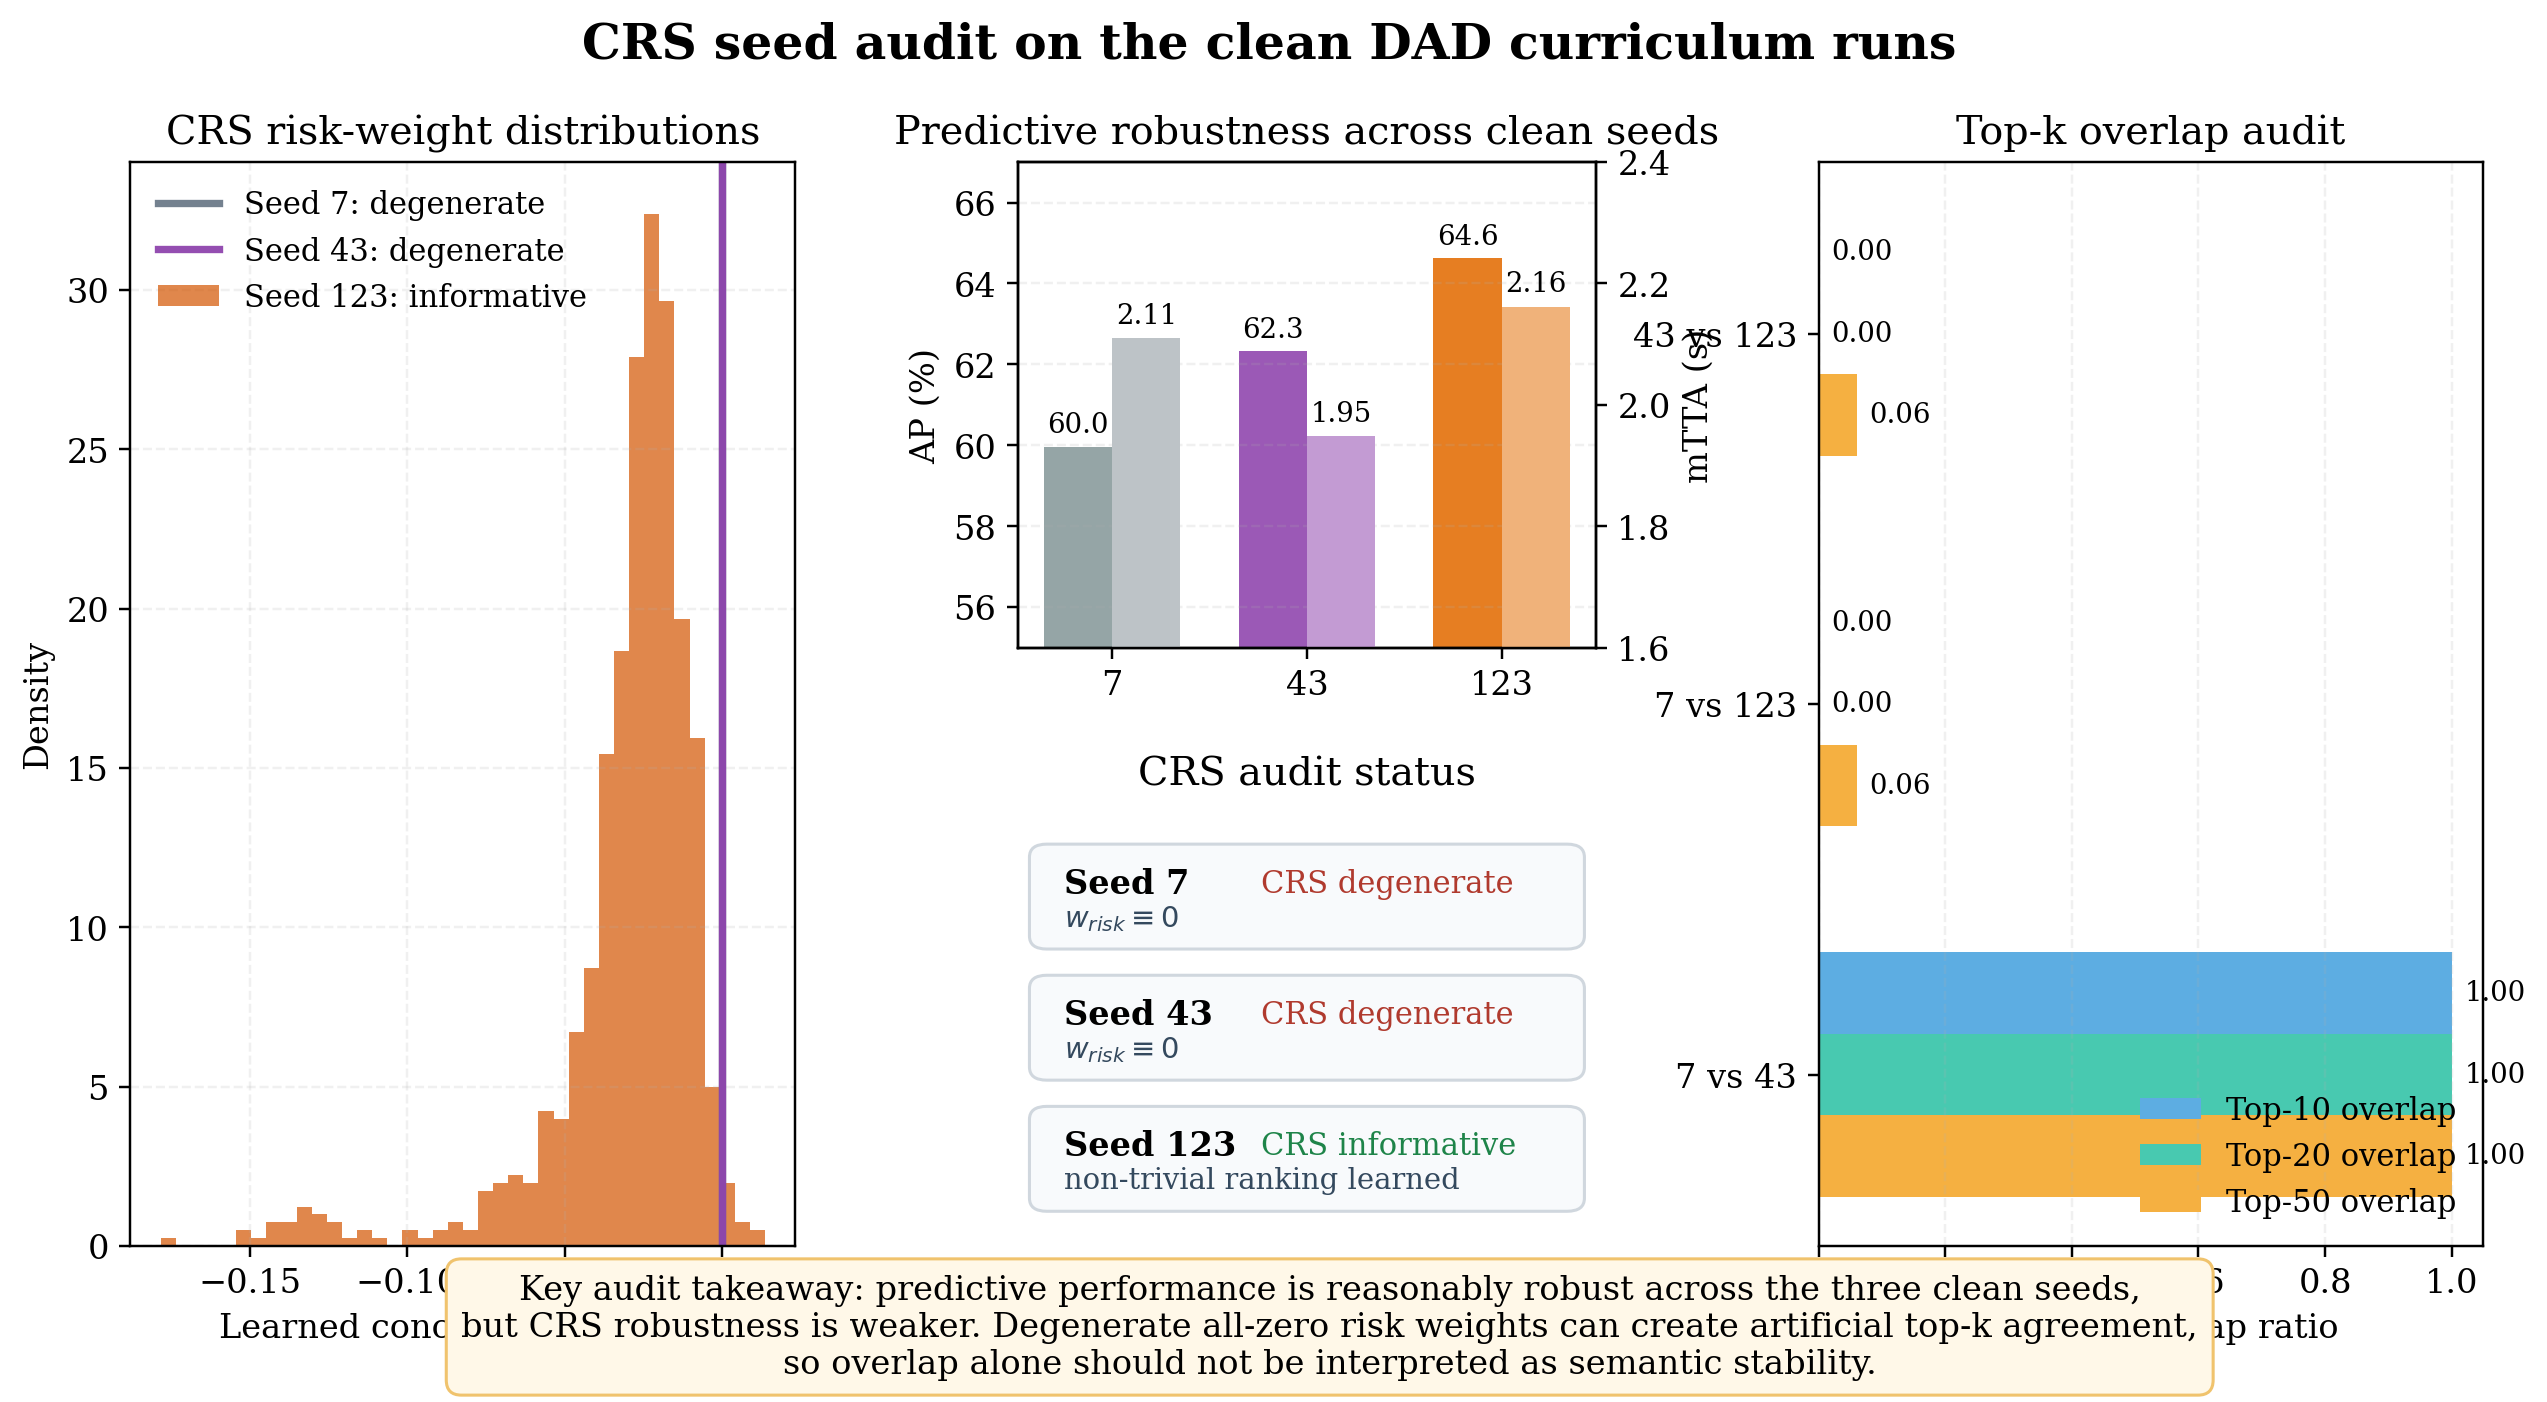
\includegraphics[width=0.98\linewidth]{../figures/insight_fig_appendix_crs_seed_audit.pdf}
  \caption{\textbf{CRS seed audit on the clean DAD curriculum runs.}
  Left: the learned CRS risk-weight distribution is degenerate for seeds 7 and
  43 (all-zero weights), while seed 123 learns a non-trivial ranking.
  Middle: predictive metrics remain reasonably similar across seeds, showing
  that predictive robustness and CRS robustness are not the same phenomenon.
  Right: pairwise top-$k$ overlap is high only for the degenerate pair and
  collapses against the informative seed, so overlap alone should not be read
  as evidence of semantic stability.}
  \label{fig:appendix_crs_seed_audit}
\end{figure}

\paragraph{Why this CRS audit matters.}
Reviewer-facing stability claims should distinguish \emph{predictive robustness}
from \emph{CRS robustness}. The three clean DAD seeds remain useful for the
former, but Table~\ref{tab:crs_seed_audit} and
Figure~\ref{fig:appendix_crs_seed_audit} show that they do not yet support a
strong claim that the learned concept-risk ranking is stable across seeds.
In particular, two of the three clean seeds are degenerate, while only one
learns a non-trivial CRS ranking. This means the current clean-seed degeneracy
rate is $2/3$, and it also means that top-$k$ overlap and family-level
agreement are not genuinely informative stability statistics at present because
there is only one informative seed in the audited pool. This motivates the
paper's current cautious wording: the semantic interface is architecturally
meaningful and partially supported quantitatively, but CRS should currently be
understood as a \emph{tentative audit signal} rather than as a mature,
deployment-ready inspector interface. A stronger multi-seed CRS stability study
should therefore be viewed as an explicit next validation target rather than as
a completed result.

\paragraph{Trigger-source support beyond one checkpoint.}
We also extended the actor-versus-classifier comparison beyond the single
representative DAD checkpoint used in the main table. Across six same-family
curriculum checkpoints, classifier-based trigger evaluation averages
$61.11\%\pm4.58$ AP and $2.17\pm0.19$~s mTTA, while actor-based trigger
evaluation averages $37.41\%\pm7.35$ AP and $3.73\pm1.39$~s mTTA. The mean
actor threshold-crossing rate at $0.5$ is only $0.68\pm0.43$, which exposes a
second source of instability: even when the actor emits usable timing behavior
on some checkpoints, its crossing dynamics are not yet consistent enough to
serve as the main paper metric path.

\subsection{Concept Ontology Construction: Additional Details}
\label{app:concept_pipeline}

\paragraph{Why this appendix section matters.}
A natural concern is whether our concepts are merely a fixed word list
chosen by hand. The answer is no. The current project contains a full pipeline
for constructing and comparing accident-risk ontologies, and this appendix
makes that process explicit so that the semantic interface of \method{} can be
audited as carefully as the neural architecture itself.

\paragraph{Ontology evolution across stages.}
Table~\ref{tab:concept_evolution} summarises the ontology evolution that is
actually relevant for the current paper. The progression is now sharper than in
earlier drafts: we begin with a broad historical vocabulary for high-coverage
training, keep a compact manual risk-core set as a human-prior baseline, and
then construct a paper-ready discovered ontology through large-vocabulary
mining, risk-first consolidation, family balancing, naming normalization, and
very-light human review. Figure~\ref{fig:concept_evolution} complements the
table with representative examples from these stages, while
Figure~\ref{fig:concept_case_study} makes the merge provenance concrete through
real canonicalization examples.

\begin{figure*}[t]
  \centering
  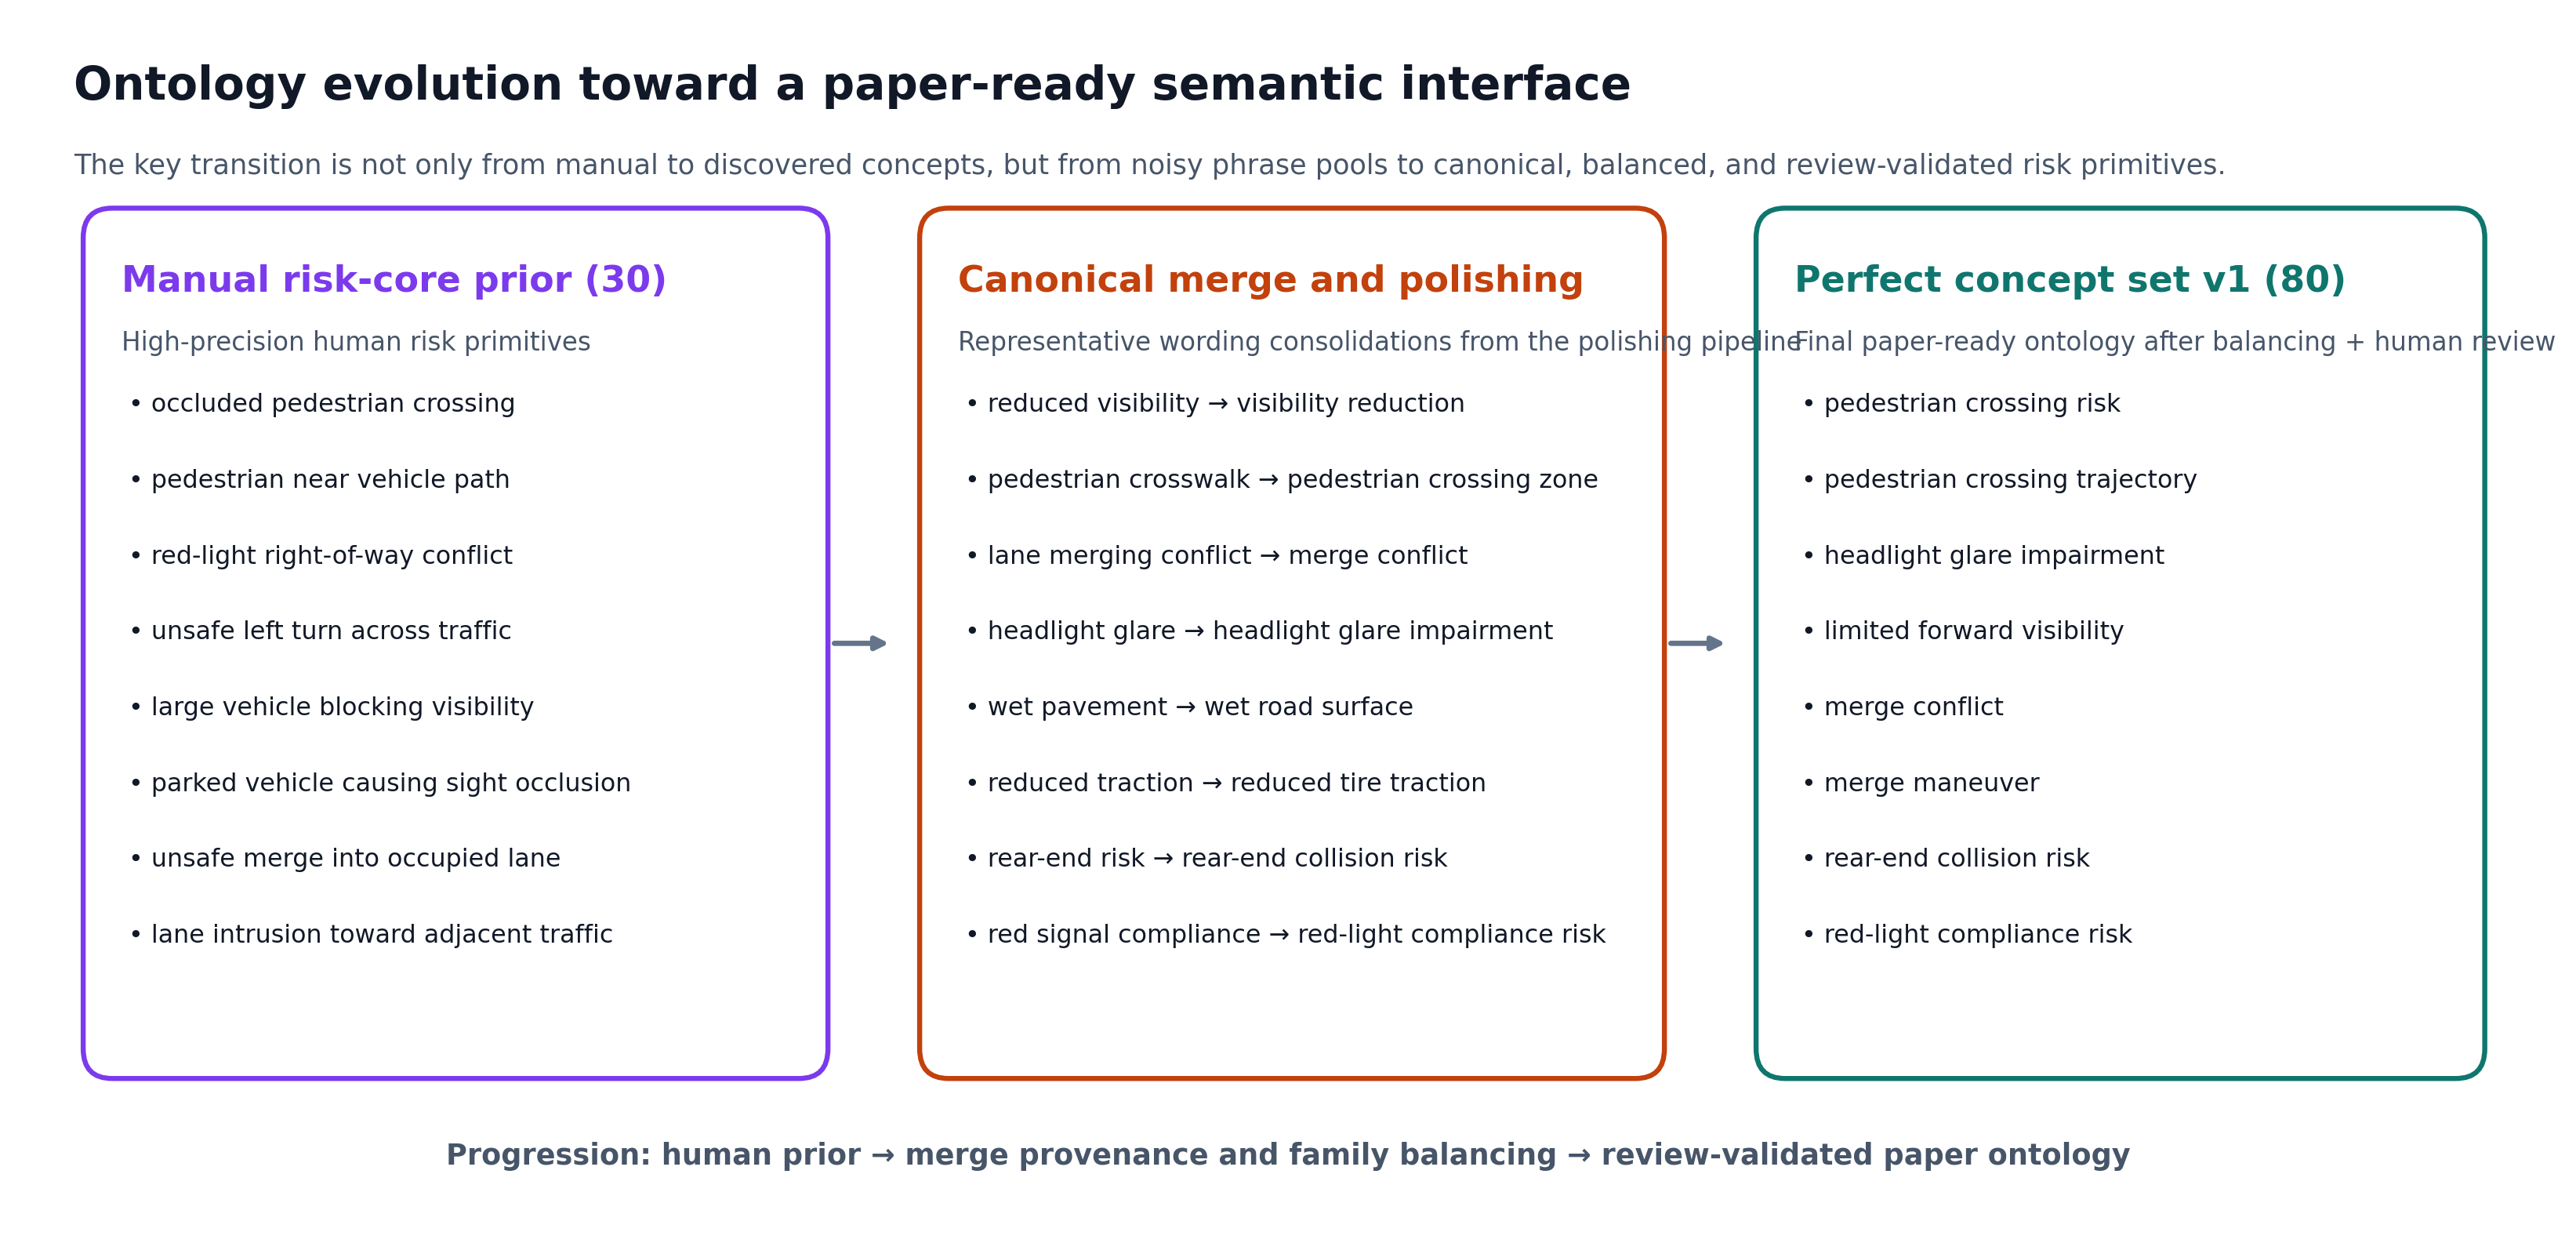
\includegraphics[width=0.98\textwidth]{../figures/insight_fig_concept_evolution.pdf}
  \caption{\textbf{Ontology evolution toward a paper-ready semantic interface.}
  Left: the manual risk-core ontology encodes strong human priors about accident
  precursors. Middle: representative merge and canonicalization examples from
  the polishing pipeline show how noisy or fragmented phrase clusters are
  compressed into stable risk primitives. Right: the final \emph{Perfect concept
  set v1} provides a balanced and review-validated ontology that is both more
  readable than the broad historical pool and more mature than early compact
  discovered pilots.}
  \label{fig:concept_evolution}
\end{figure*}

\begin{table}[t]
\caption{Concept ontology evolution across the project.}
\label{tab:concept_evolution}
\centering\small
\setlength{\tabcolsep}{4pt}
\resizebox{\linewidth}{!}{%
\begin{tabular}{lccp{0.42\linewidth}}
\toprule
Stage & \#Concepts & Source & Main property \\
\midrule
Historical full vocabulary & 837 & Broad CLIP-derived concept bank & High coverage, historically strongest CBM line, but semantically noisy and too large for clean paper presentation \\
Risk-core manual set & 30 & Manual risk-first curation & High-precision compact human prior over accident precursors \\
Perfect concept set v1 & 80 & Large-vocab discovery + polishing + human review & Balanced paper-ready ontology with canonical naming, merge provenance, explicit family coverage, and exhaustive per-concept review \\
\bottomrule
\end{tabular}%
}
\end{table}

\paragraph{Controlled ontology block status.}
The shared-launcher ontology comparison described in the main paper is now
complete as an artifact block: all six recommended runs
(\texttt{DAD/A3D} crossed with \texttt{historical\_full},
\texttt{risk\_core\_v1}, and \texttt{perfect\_v1}) are present with stored
checkpoints and \texttt{results.json} summaries. This matters because the
ontology claim is no longer resting on planned compute. On DAD, the compact
manual ontology achieves the highest AP while the polished discovered ontology
achieves the best mTTA; on A3D, the polished ontology achieves the strongest AP
while the compact manual ontology gives the best timing metrics. In other
words, the appendix now supports the main-paper reading directly: ontology
choice changes the operating point under one matched recipe.

The seed-backed extension of this block is also complete: all $18/18$
recommended seeded ontology runs have finished. This matters because the
ontology claim no longer depends on a half-completed follow-up.
The aggregate picture is consistent with the main paper's interpretation. On
A3D, the polished discovered ontology remains a strong AP-oriented operating
point under three seeds ($93.35\%\pm0.49$ AP), while on DAD the same ontology
is visibly more variable ($60.11\%\pm7.40$ AP). We therefore read the multi-seed
results as strengthening the ontology-science claim while also sharpening the
paper's limitation statement: the semantic interface looks materially more
stable on A3D than on DAD.

\paragraph{Prompt template design.}
Our prompts explicitly instruct the multimodal model to prioritise
\emph{safety-relevant early cues} rather than generic scene description.
Representative output fields include a compact concept phrase, a short risk
rationale, and a semantic family tag. A simplified prompt sketch is:
\begin{quote}
``Given a pre-crash driving frame, list short risk concepts that could function
as accident precursors. Prefer dynamic hazard cues, proximity conflict,
visibility degradation, braking or cut-in behaviour, and lane-level conflict.
Avoid generic objects or background scene tags unless they directly contribute
to accident risk.''
\end{quote}
We pair this instruction with a structured JSON schema so that outputs can be
programmatically filtered, clustered, and adjudicated. A representative schema
fragment is shown below.

\begin{quote}
\small
\noindent\parbox{0.95\linewidth}{\raggedright\ttfamily
\{"frame\_id": "dad\_xxx\_f042",\\
"risk\_concepts": [\\
\hspace*{1em}\{"concept": "trajectory conflict",\\
\hspace*{2em}"family": "motion\_conflict",\\
\hspace*{2em}"why\_risky": "vehicles are converging into\\
\hspace*{2em}the same path"\},\\
\hspace*{1em}\{"concept": "forward visibility limit",\\
\hspace*{2em}"family": "visibility",\\
\hspace*{2em}"why\_risky": "driver cannot reliably\\
\hspace*{2em}anticipate hidden hazards"\}\\
],\\
"discarded\_scene\_tags": ["road", "car", "intersection"]\\
\}}
\normalsize
\end{quote}

\paragraph{Concrete examples from the current polishing pipeline.}
The manual risk-core set contains phrases such as \emph{lane intrusion toward
adjacent traffic}, \emph{oncoming-traffic conflict}, and \emph{large vehicle
blocking visibility}. The newer large-vocabulary discovery stage produces a
much broader phrase pool that includes many useful but fragmented variants,
such as \emph{reduced visibility}, \emph{pedestrian crosswalk},
\emph{lane merging conflict}, or \emph{wet pavement}. The polishing stage then
consolidates these into canonical training-ready forms such as
\emph{visibility reduction}, \emph{pedestrian crossing zone},
\emph{merge conflict}, and \emph{wet road surface}. Including both raw and
canonical forms is important: it shows how the pipeline moves from high-recall
multimodal phrase mining toward a smaller, more stable, and more reviewable
ontology without losing the underlying risk semantics.

\paragraph{Failure modes in raw discovery.}
The raw discovery stage is intentionally high recall and therefore noisy.
Typical failure modes include: (i) generic object mentions that carry little
predictive value (e.g., ``road'', ``vehicle''), (ii) visually salient but weakly
risk-relevant background phrases, (iii) duplicate concepts with slightly different
wording, and (iv) over-specific phrases that do not transfer across clips.
These failure modes are precisely why the refinement and adjudication stages
are necessary; they are not implementation accidents, but expected properties
of an intentionally recall-heavy front end.

\paragraph{Why polishing plus human review is useful.}
The final ontology stage does more than clean spelling. It rebalances semantic
families, collapses near-synonyms, enforces canonical naming, and applies a
very-light human review over every retained concept. This matters for both
science and engineering: the method needs a reproducible ontology with visible
provenance, and the downstream model wants a small set of stable concepts
rather than a fragile bag of aliases. Figure~\ref{fig:concept_case_study} shows
representative real merge examples from this process, moving from noisy raw
multimodal phrases to final canonical concepts that can be presented in the
paper and used directly for downstream CBM training.

The current audit trail makes this concrete. Starting from 611 mined phrases,
the polishing pipeline compresses the pool to 81 post-polish canonical
candidates and a finalized paper release of 80 retained concepts. The review
record spans all 80 retained concepts across nine semantic families, and the
documented decisions are intentionally light-touch: wording is checked and
canonicalized, but the ontology is not rebuilt by hand. This is the level of
governance we want the paper to claim: explicit canonical naming, visible merge
provenance, and family balance that can be inspected by a reader without
pretending that the vocabulary is a finished standalone linguistic resource.

\paragraph{What the language-side evidence is meant to establish.}
The paper does not claim that these canonical names are universally optimal or
that the ontology has become a finished linguistic resource. The narrower and
more defensible claim is that the ontology is governed enough to function as a
scientific interface: canonical names remain reasonably stable under light
paraphrase variation, semantic families are explicit rather than implicit, and
merge choices are reviewable rather than hidden inside prompt iteration.

\begin{figure*}[t]
  \centering
  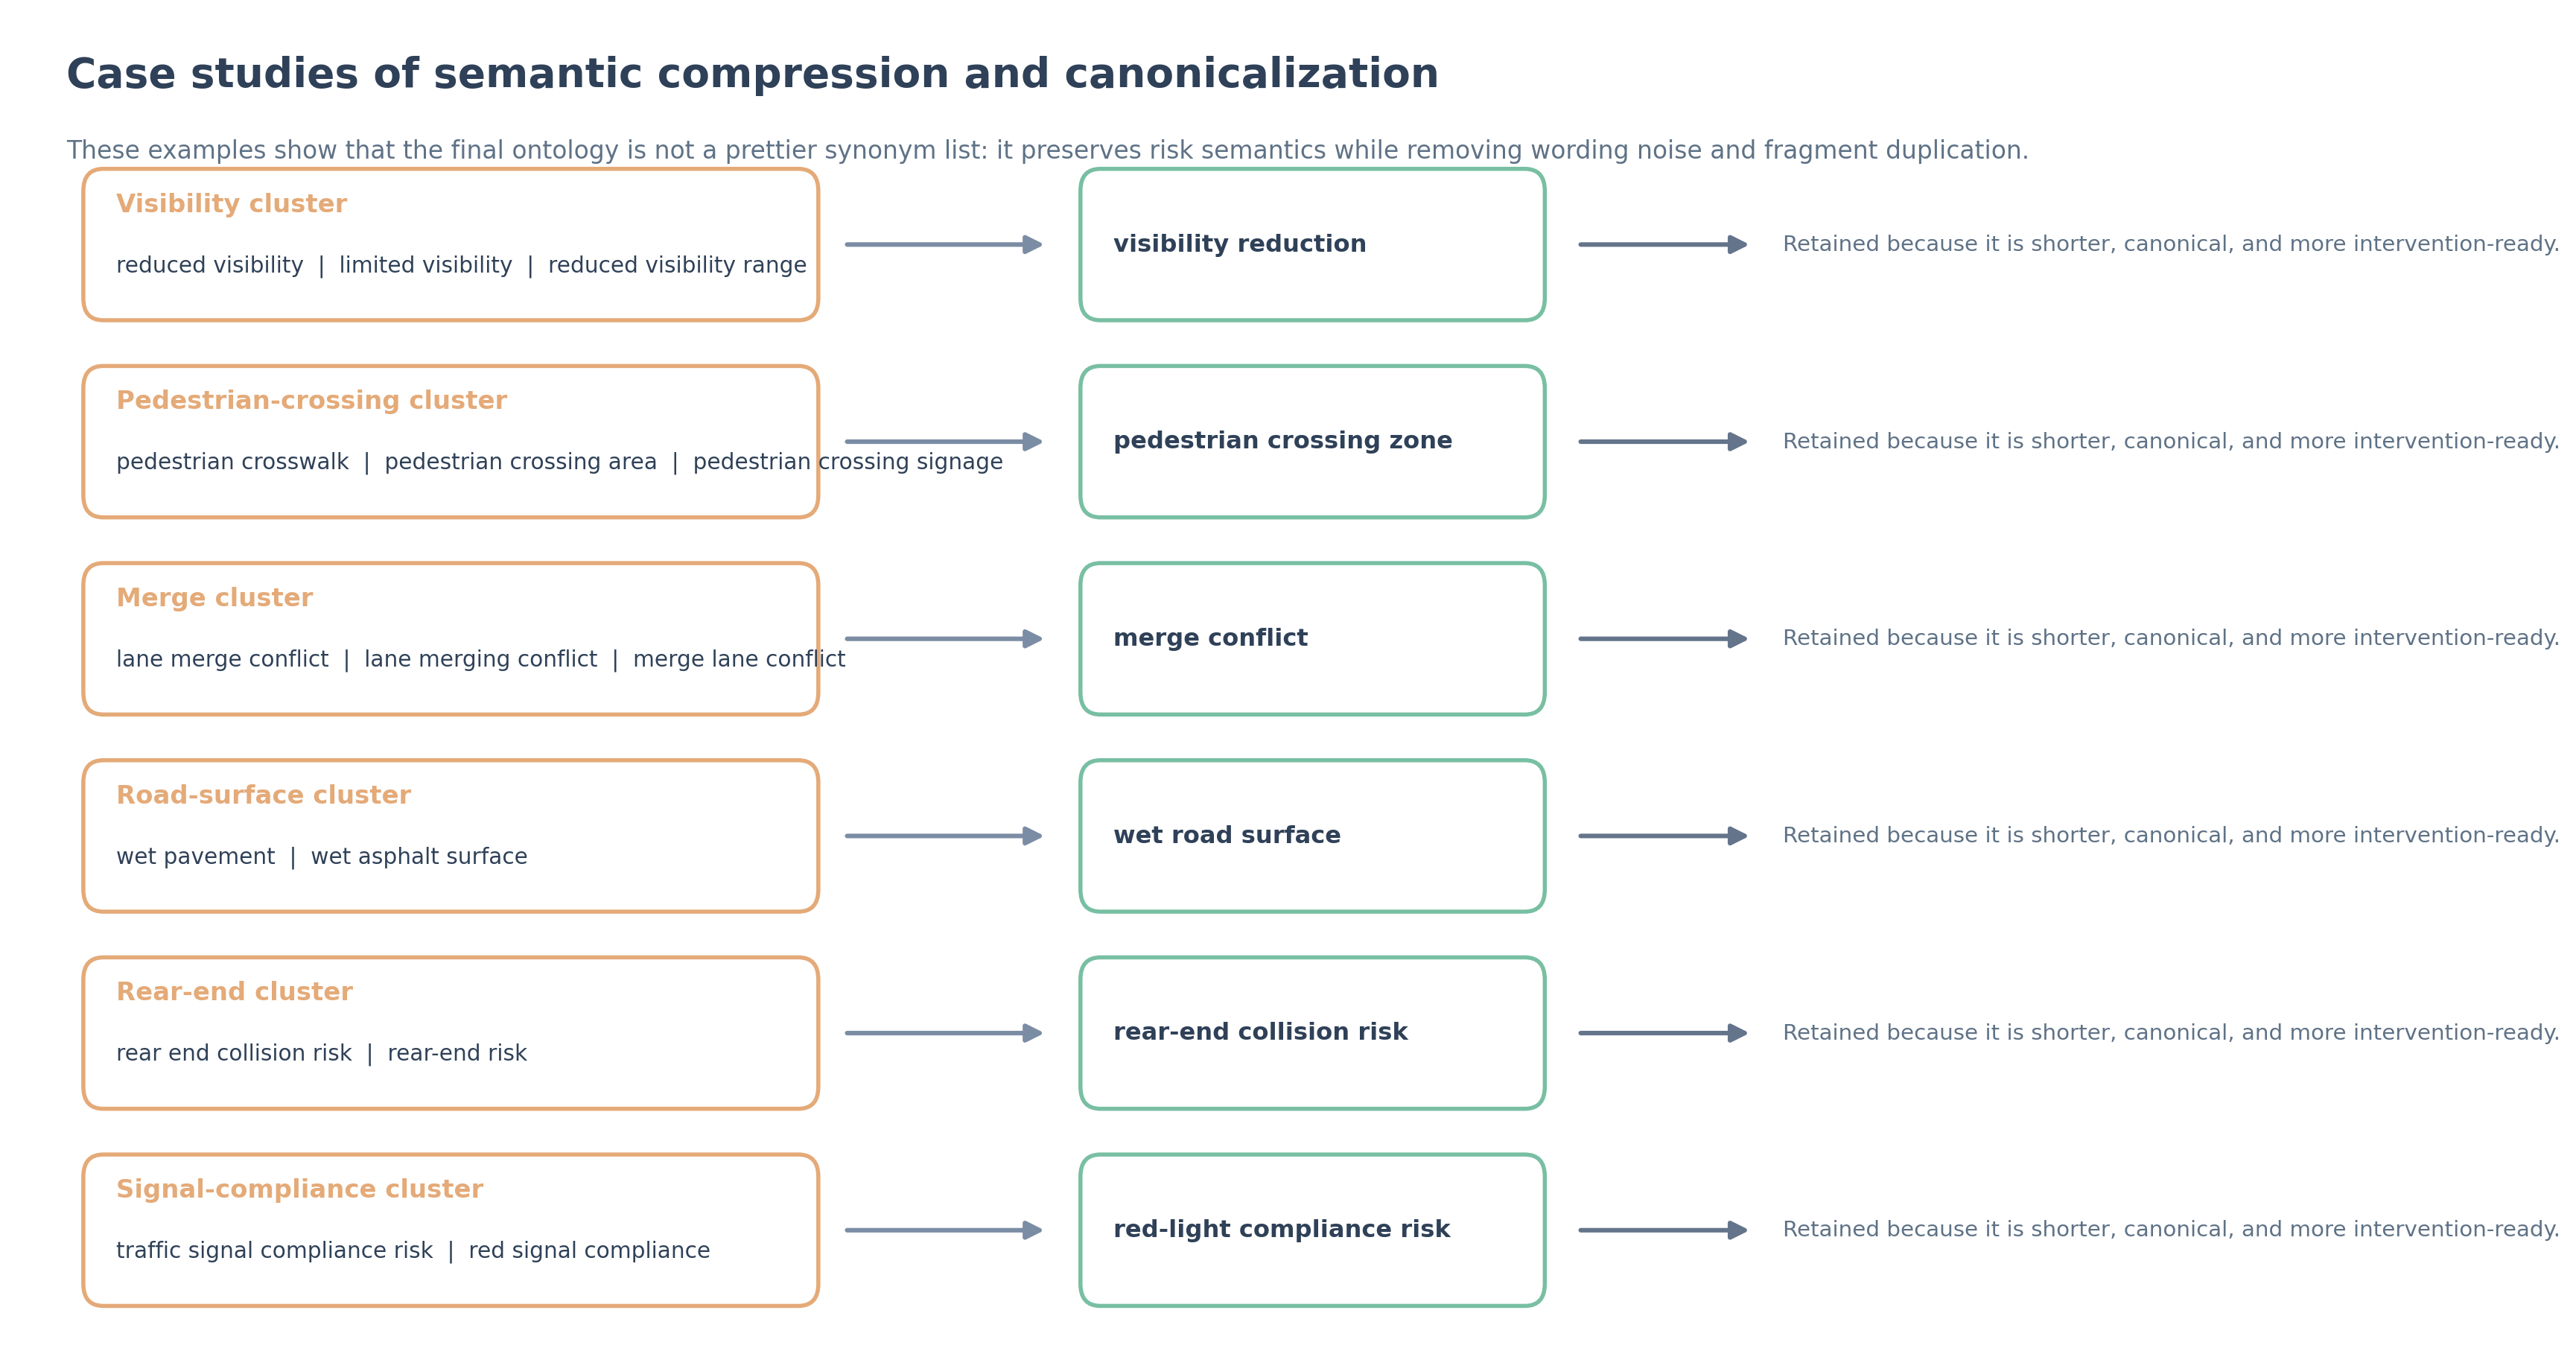
\includegraphics[width=0.98\textwidth]{../figures/insight_fig_concept_case_study.pdf}
  \caption{\textbf{Case studies of semantic compression and canonicalization.}
  Each row shows a representative merge path from noisy or fragmented phrase
  variants to a single canonical paper-ready concept. These examples make two
  points explicit: the pipeline removes lexical fragmentation, and the final
  ontology is not merely a prettier synonym list but a more stable semantic
  interface for downstream CBM training, family-level analysis, and external
  auditing.}
  \label{fig:concept_case_study}
\end{figure*}

\paragraph{What counts as success.}
A discovered concept set is successful only if it satisfies four criteria:
(1) semantic plausibility to a human reader, (2) coverage of major accident
precursor families, (3) trainability in the downstream CBM pipeline, and
(4) auditability at the paper level through family metadata, merge provenance,
and human review. This is why the paper reports not only ontology examples and
downstream training results, but also family-balance figures and merge case
studies. A pretty concept list without learning value is not enough; conversely,
a trainable but uninterpretable list would defeat the purpose of the semantic
interface.

\begin{figure}[t]
  \centering
  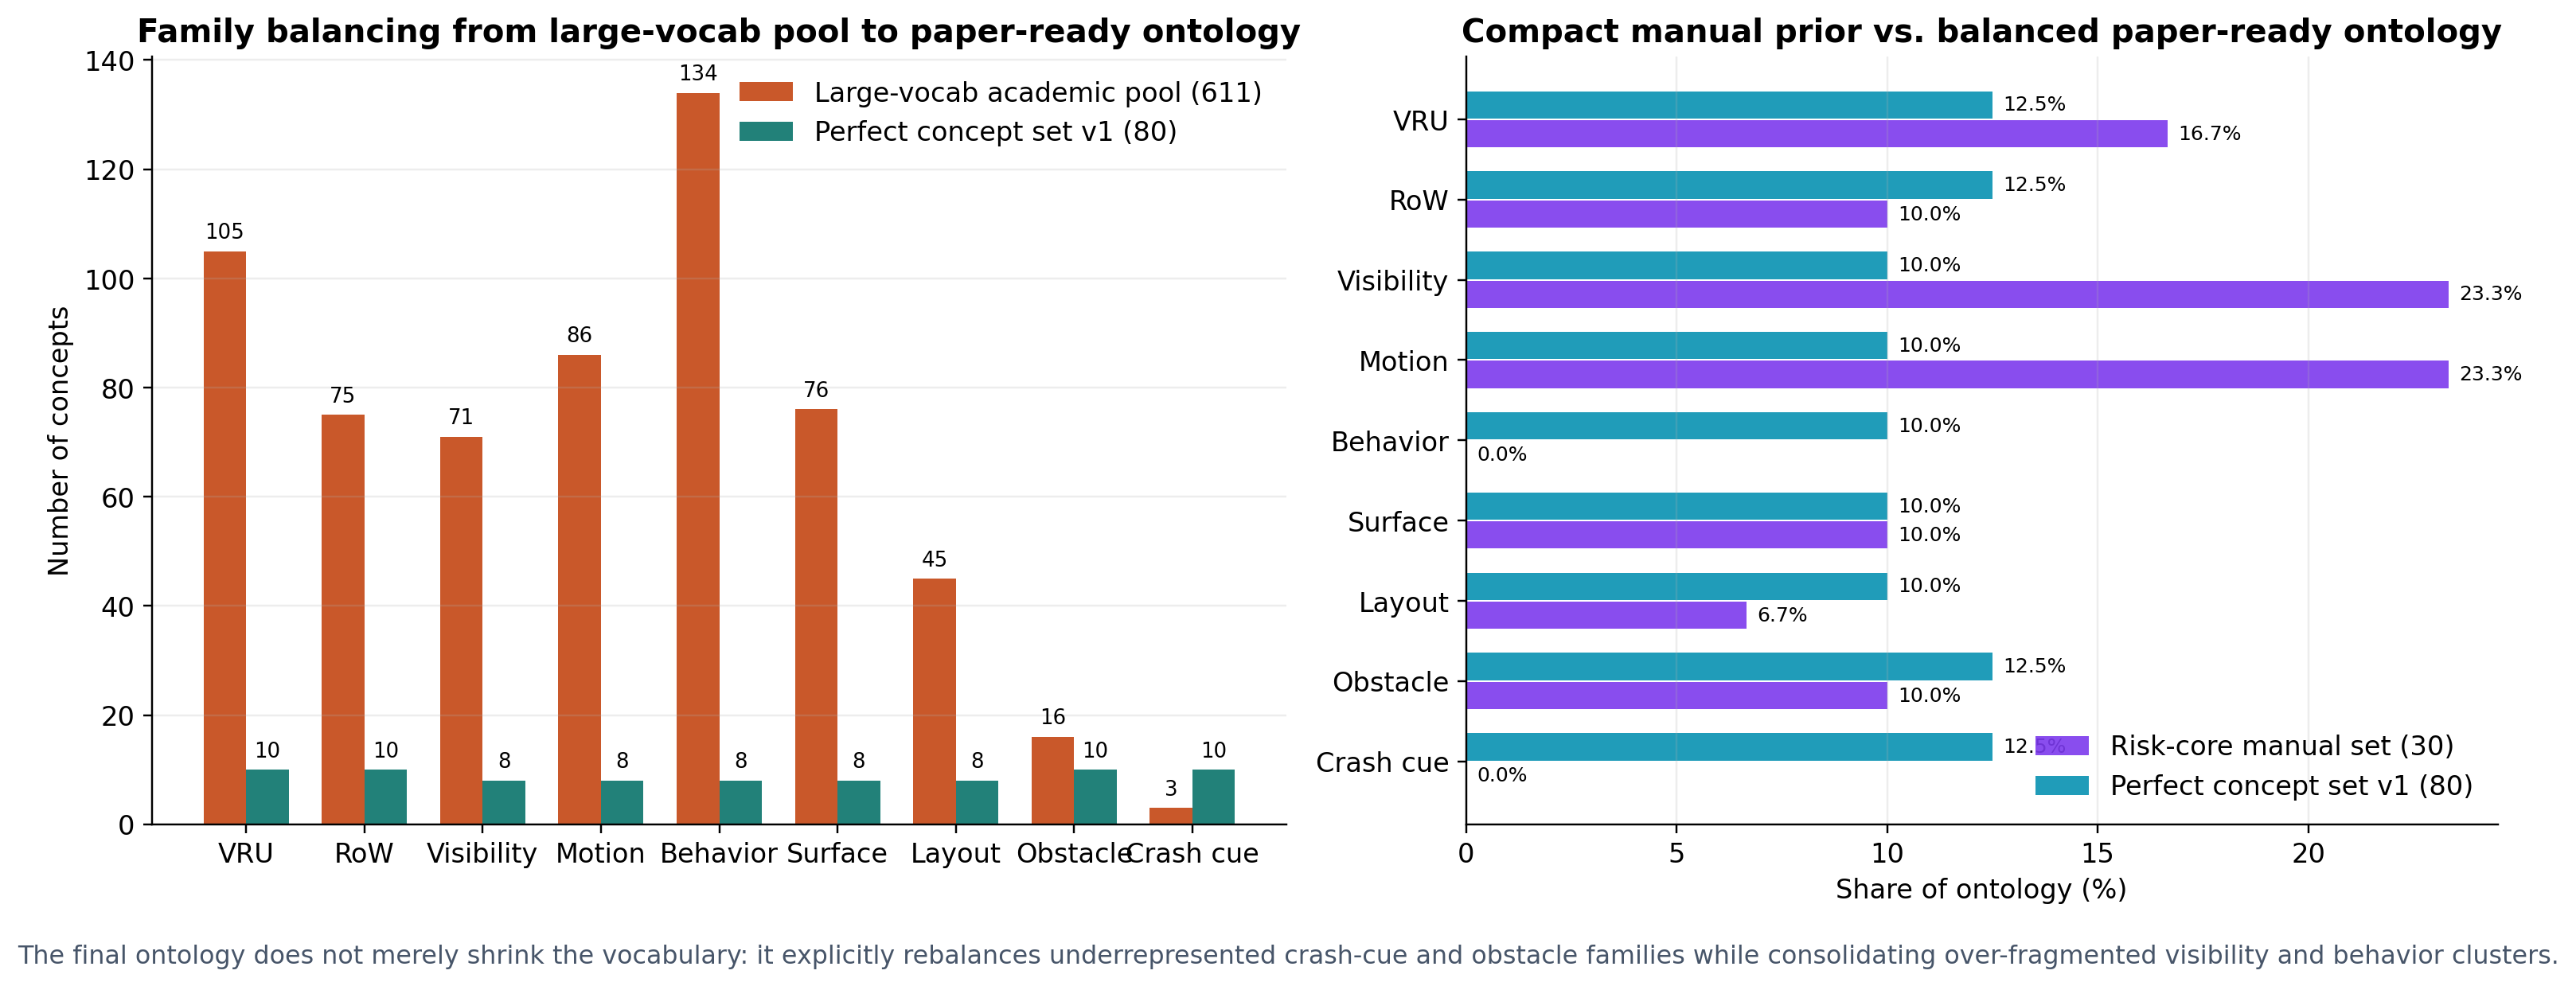
\includegraphics[width=0.98\linewidth]{../figures/insight_fig_concept_family_coverage.pdf}
  \caption{\textbf{Family coverage before and after ontology polishing.}
  The broad large-vocabulary pool is highly imbalanced, while the final paper-ready
  ontology explicitly rebalances crash-cue, obstacle, and vulnerable-road-user
  families without collapsing the ontology into a tiny manually curated list.
  This supports our claim that ontology polishing is not cosmetic compression;
  it is a structured operation that improves auditability and semantic balance.}
  \label{fig:concept_family_coverage}
\end{figure}

\subsection{Why the Semantic Interface Can Affect Timing}
\label{app:theory}

\paragraph{From latent prediction to semantic decision-making.}
A conventional recurrent anticipation model compresses all evidence into a
single latent state $\mathbf{h}_t$ and predicts risk from that state alone.
This is often sufficient for raw prediction, but it is weak from an auditing
perspective because the model offers no explicit separation between
\emph{evidence extraction} and \emph{decision timing}. By contrast, \method{}
explicitly decomposes these two roles:
\begin{itemize}[leftmargin=1.5em]
  \item the \textbf{semantic layer} estimates a concept state $\mathbf{c}_t$ that
  summarises semantically meaningful risk evidence, and
  \item the \textbf{timing layer} learns a timing policy over a concept-aware
  sequential state $\mathbf{s}_t=[\mathbf{h}_t\|\mathbf{c}_t]$.
\end{itemize}
This decomposition is not cosmetic. It changes the information geometry of the
problem: the policy no longer acts on an opaque hidden vector alone, but on a
state with an explicit semantic interface.

\paragraph{A simple monotonicity view.}
Suppose the concept state contains one or more dimensions corresponding to
hazard indicators whose increase is semantically consistent with increasing
risk. If the downstream timing policy is trained to reward earlier correct
alerts, then a policy conditioned on $\mathbf{s}_t=[\mathbf{h}_t\|\mathbf{c}_t]$
can, in principle, cross the alert boundary before a purely confidence-based
predictor reaches its peak. Informally, the concept channel acts as an early
warning basis: a rise in concept evidence can move the system toward action
before the latent classifier has accumulated maximal confidence. This is the
core reason the semantic and timing layers are coupled but not redundant.

\paragraph{Why intervention is meaningful.}
Let a concept edit be represented as a perturbation
$\Delta\mathbf{c}_t$ applied over a short pre-crash window.
Because the downstream predictor or policy consumes a state containing the
concept vector, the perturbation induces a corresponding perturbation in the
decision state:
\[
\mathbf{s}'_t = [\mathbf{h}_t\|\mathbf{c}_t + \Delta\mathbf{c}_t].
\]
If the architecture is truly concept-conditioned rather than merely
post-hoc-explainable, then semantically valid positive perturbations on a risk
concept should induce a stronger or earlier warning response at the output.
This is why the intervention analysis is an architectural test, not just a
visualisation trick. The test asks whether the semantic interface has
non-trivial structured influence on the decision pathway.

\paragraph{What this appendix-level analysis does and does not claim.}
We do not claim a formal global theorem guaranteeing monotone policy shifts for
all concept edits, since the recurrent dynamics and nonlinearities are too rich
for such a guarantee to be informative without unrealistic assumptions. The
point of the analysis is instead to make clear why the design is principled:
separating semantic evidence estimation from timing control creates a decision
pathway that is inspectable, perturbable, and therefore much closer to the
needs of safety auditing than a single black-box recurrent score.

\subsection{Scoped Intervention Evidence}
\label{app:intervention}

A standard promise of concept bottleneck models is \emph{intervenability}: a
human can inspect a concept, judge that it is mis-estimated, and correct it
without retraining the full network. For accident anticipation, this capability
is especially important because many practically relevant errors are not
arbitrary; they are tied to under-activation of an intuitively correct risk
concept. In the current paper, however, intervention should be read as
\emph{support evidence} for a meaningful semantic control surface, not as a
completed policy-level causal benchmark.

\begin{figure*}[t]
  \centering
  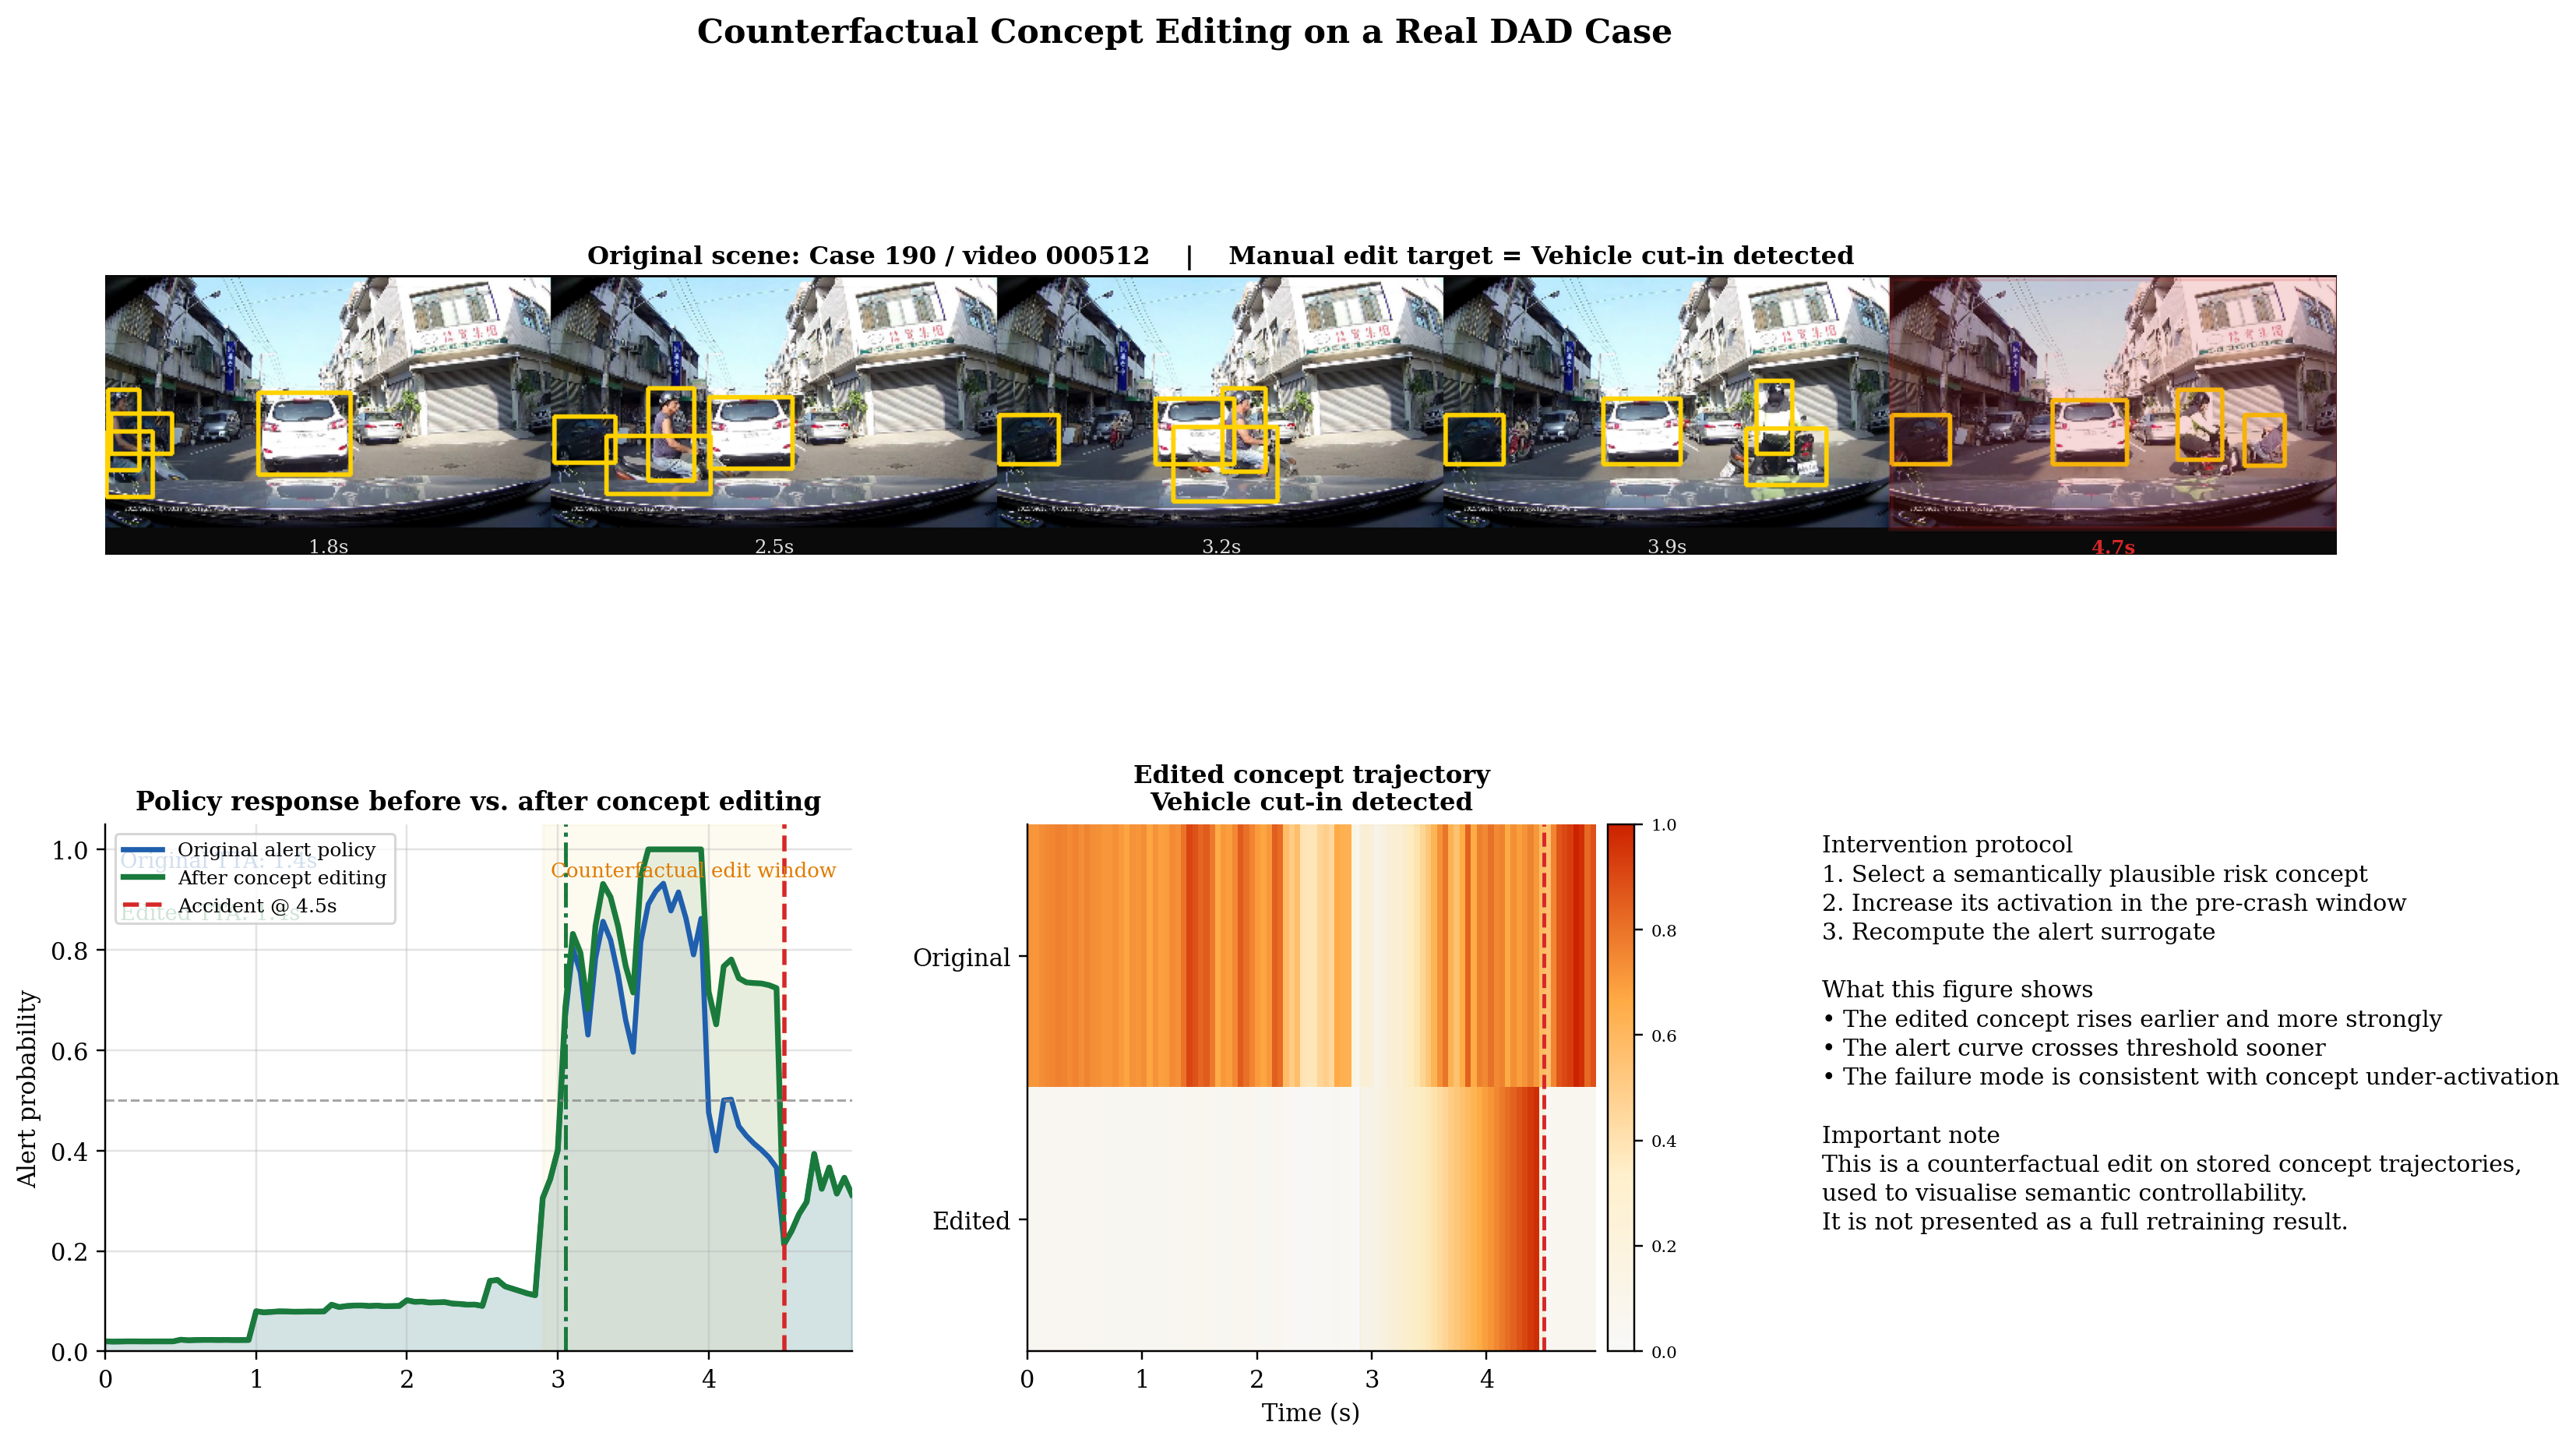
\includegraphics[width=\textwidth]{../figures/insight_fig_appendix_intervention.pdf}
  \caption{\textbf{Counterfactual concept editing on a DAD case.}
A semantically plausible pre-crash concept trajectory is increased and the
resulting warning surrogate is recomputed. The edited concept rises earlier,
and the alert curve crosses threshold sooner. This figure is intentionally a
stored-trajectory counterfactual rather than a full model re-run; its role is
to show that the model exposes a semantically meaningful control surface.}
  \label{fig:appendix_intervention}
\end{figure*}

\paragraph{Stored-trajectory intervention protocol.}
For a false-negative or borderline DAD case, we select a concept whose
activation is visibly inconsistent with the scene semantics, increase it over
the pre-crash window, and compare the original and edited warning trajectories.
This directly tests whether strengthening the right concept can move the
warning earlier.

\paragraph{Outcome.}
Figure~\ref{fig:appendix_intervention} shows that it can. The edited alert
curve rises and crosses threshold earlier than the original one. Across the
archived quantitative summaries, however, the effect remains heterogeneous. In
the strongest archived hybrid-boost setting, the mean alert shift is
$-2.04$ frames over 64 cases, but the median shift is still 0.0; by contrast,
both the null-style hybrid baseline and the risk-weight baseline produce a mean
shift of 0.0 over 32 cases each. The correct interpretation is therefore
\emph{partial structural intervenability} rather than a completed causal proof.

\begin{figure*}[t]
  \centering
  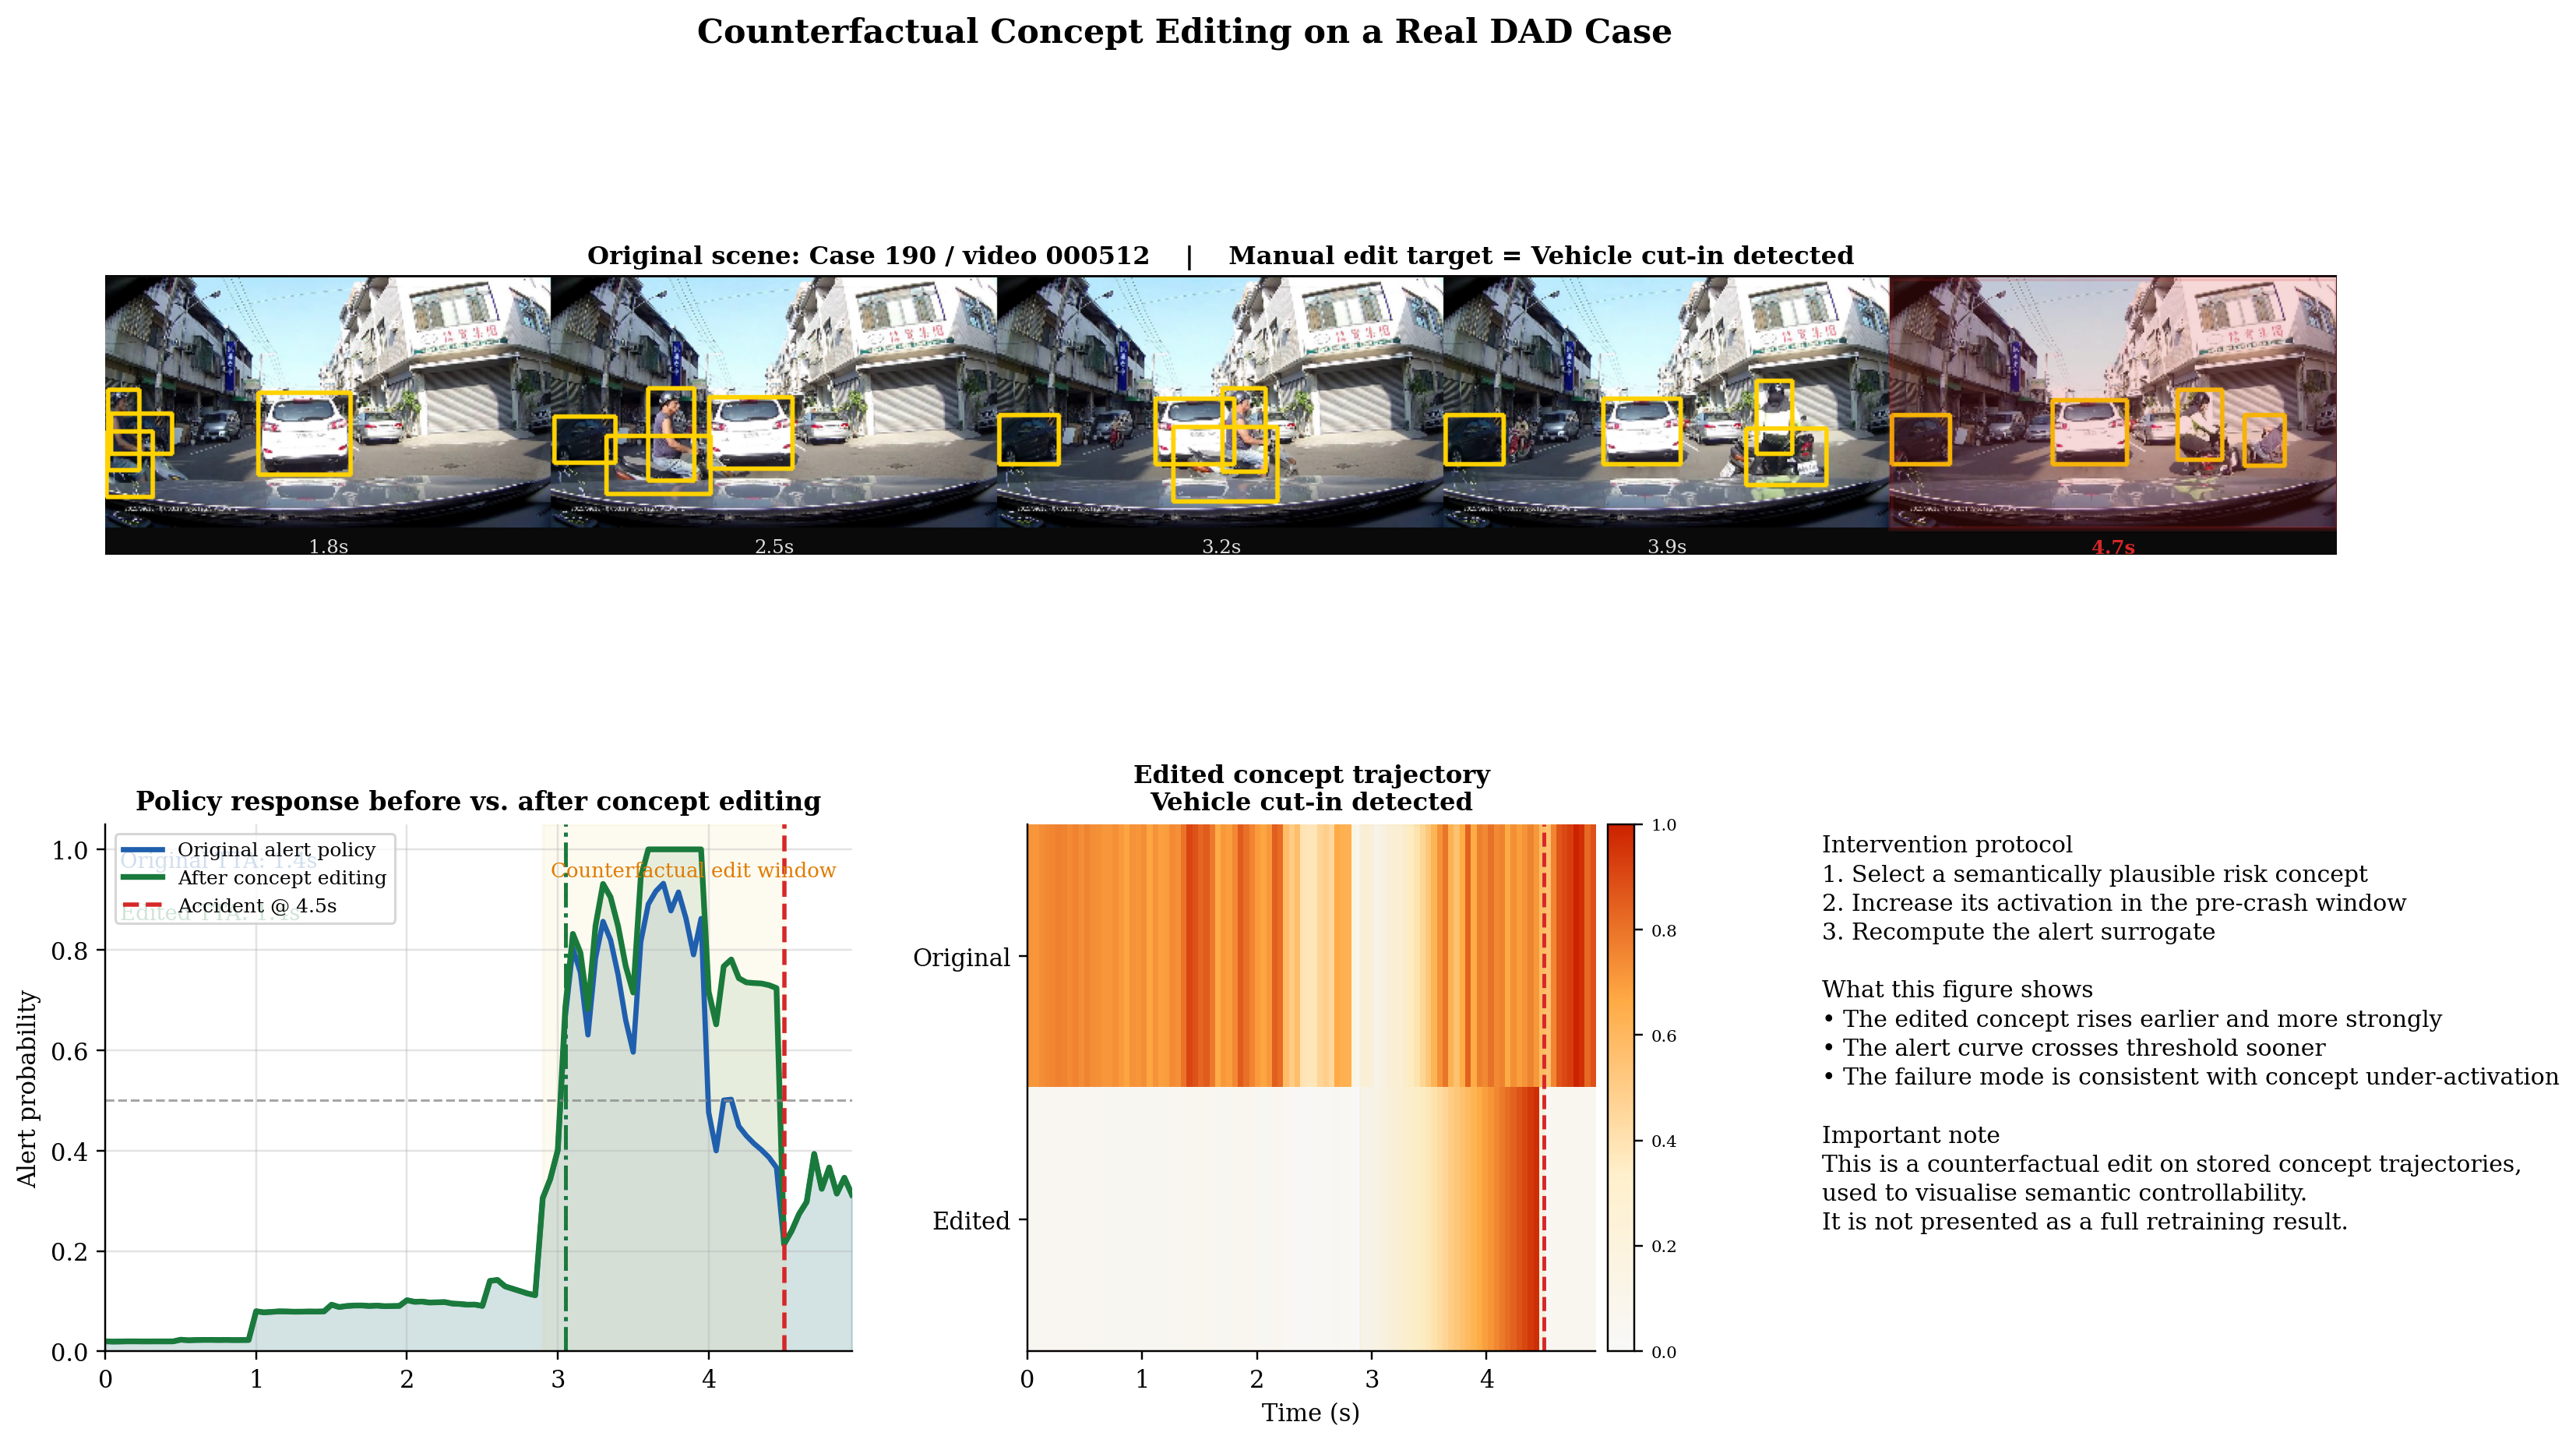
\includegraphics[width=\textwidth]{../figures/insight_fig_appendix_intervention_v4_backbone.pdf}
  \caption{\textbf{Backbone-level intervention re-run with the v4 DAD checkpoint.}
A concept channel is edited in the pre-crash window and the downstream
prediction branch is recomputed through the loaded backbone. This is a stronger
intervention path than stored-trajectory editing, but it is still not a full
policy-level intervention because the available checkpoint lacks the final
Actor--Critic head weights.}
  \label{fig:appendix_intervention_v4}
\end{figure*}

\paragraph{Backbone-level re-run.}
To go beyond stored-trajectory editing, we also run a backbone-level
intervention using the newer DAD line. The available checkpoint loads the
concept bottleneck, temporal modules, and recurrent backbone, but not the final
Actor--Critic head weights. We therefore edit one concept channel and recompute
the downstream prediction branch through the loaded backbone.

\paragraph{Interpretation.}
The backbone-level re-run shows that concept edits remain meaningful when
propagated back through the loaded model rather than only visualised post hoc.
It also makes the current evidence boundary explicit: we can support a
concept-conditioned backbone intervention, but not yet a full policy-level
intervention without the complete Actor--Critic checkpoint.

\paragraph{Backbone-level search as a robustness check.}
To test whether Figure~\ref{fig:appendix_intervention_v4} was unusually
favourable, we also ran an automatic search across positive DAD test cases
available to that checkpoint line. For each case, we selected several
high-activity pre-crash concepts, applied graded positive edits over the
pre-crash window, and re-ran the backbone-level prediction branch. The result
is best read as an intermediate intervention audit: concept edits can propagate
through the loaded model and sometimes move warning behaviour in the expected
direction, but they do not yet support a broad claim of large or reliable
timing gains across DAD. This conclusion is reinforced by the scan artifacts:
the best stored v4 search cases mostly show no TTA improvement at all, even
when peak prediction scores shift slightly.

\subsection{Additional Qualitative Analysis}
\label{app:qual}

\begin{figure*}[t]
  \centering
  
\includegraphics[width=0.84\textwidth]{../neurips2026/dad_case_contactsheet.pdf}
  \caption{\textbf{A broader DAD case bank for qualitative screening.}
  Positive DAD test cases were ranked by a simple combination of peak risk,
  pre-crash area, and rise strength, then reviewed for visual legibility.
  The contact sheet spans different traffic geometries and visibility
  conditions, reducing the chance of a single unusually clean case driving the
  qualitative story.}
  \label{fig:appendix_casebank}
\end{figure*}

The main paper intentionally keeps the qualitative section compact. Here we
summarise the broader qualitative patterns observed across DAD cases.

\paragraph{Empirical summary of the appendix case bank.}
Taken together, the contact-sheet screening and the intervention analysis show
that the semantic interface is visible across multiple DAD scenes rather than
only in a single clean success case. At the same time, the v4 backbone search
shows that stronger concept edits do not automatically translate into large
timing shifts in every case. The appendix therefore supports both breadth of
semantic evidence and a realistic boundary on controllability.

\paragraph{Hard-case symmetry audit snapshot.}
To avoid overclaiming from qualitative examples, we maintain a separate
family-level hard-case symmetry scaffold
(`paper/neurips2026/dad_hard_case_symmetry_audit.md`) generated from archived
casebank assets. Table~\ref{tab:appendix_hard_case_symmetry} reports the
current snapshot using a primary-family heuristic and prediction-branch timing
buckets. The table is intentionally conservative: it is an audit checkpoint,
not a claim that symmetry is solved.

\begin{table}[t]
\caption{DAD hard-case symmetry audit snapshot from archived v4 casebank assets.
Counts are from the current `strong_top` pool under primary-family assignment.
`auto\_pair` denotes heuristic early-vs-late mixed pair suggestions that still
require manual reviewer confirmation.}
\label{tab:appendix_hard_case_symmetry}
\centering\small
\begin{tabular}{lrrrr}
\toprule
Primary family & Early strong & Early marginal & Late/missed & Auto pair \\
\midrule
intersection\_merge & 1 & 3 & 10 & 4 \\
visibility\_night & 0 & 0 & 6 & 0 \\
pedestrian\_conflict & 0 & 0 & 7 & 0 \\
road\_surface\_weather & 0 & 0 & 2 & 0 \\
heavy\_vehicle\_conflict & 0 & 0 & 1 & 0 \\
\bottomrule
\end{tabular}
\end{table}

This snapshot reinforces the same scope boundary used in the main paper:
current synchronized diagnostics and archived casebank evidence reveal uneven
hard-case behavior, so stronger symmetry claims remain blocked until manual
pair-level outcomes are completed in the audit file.

\begin{figure*}[t]
  \centering
  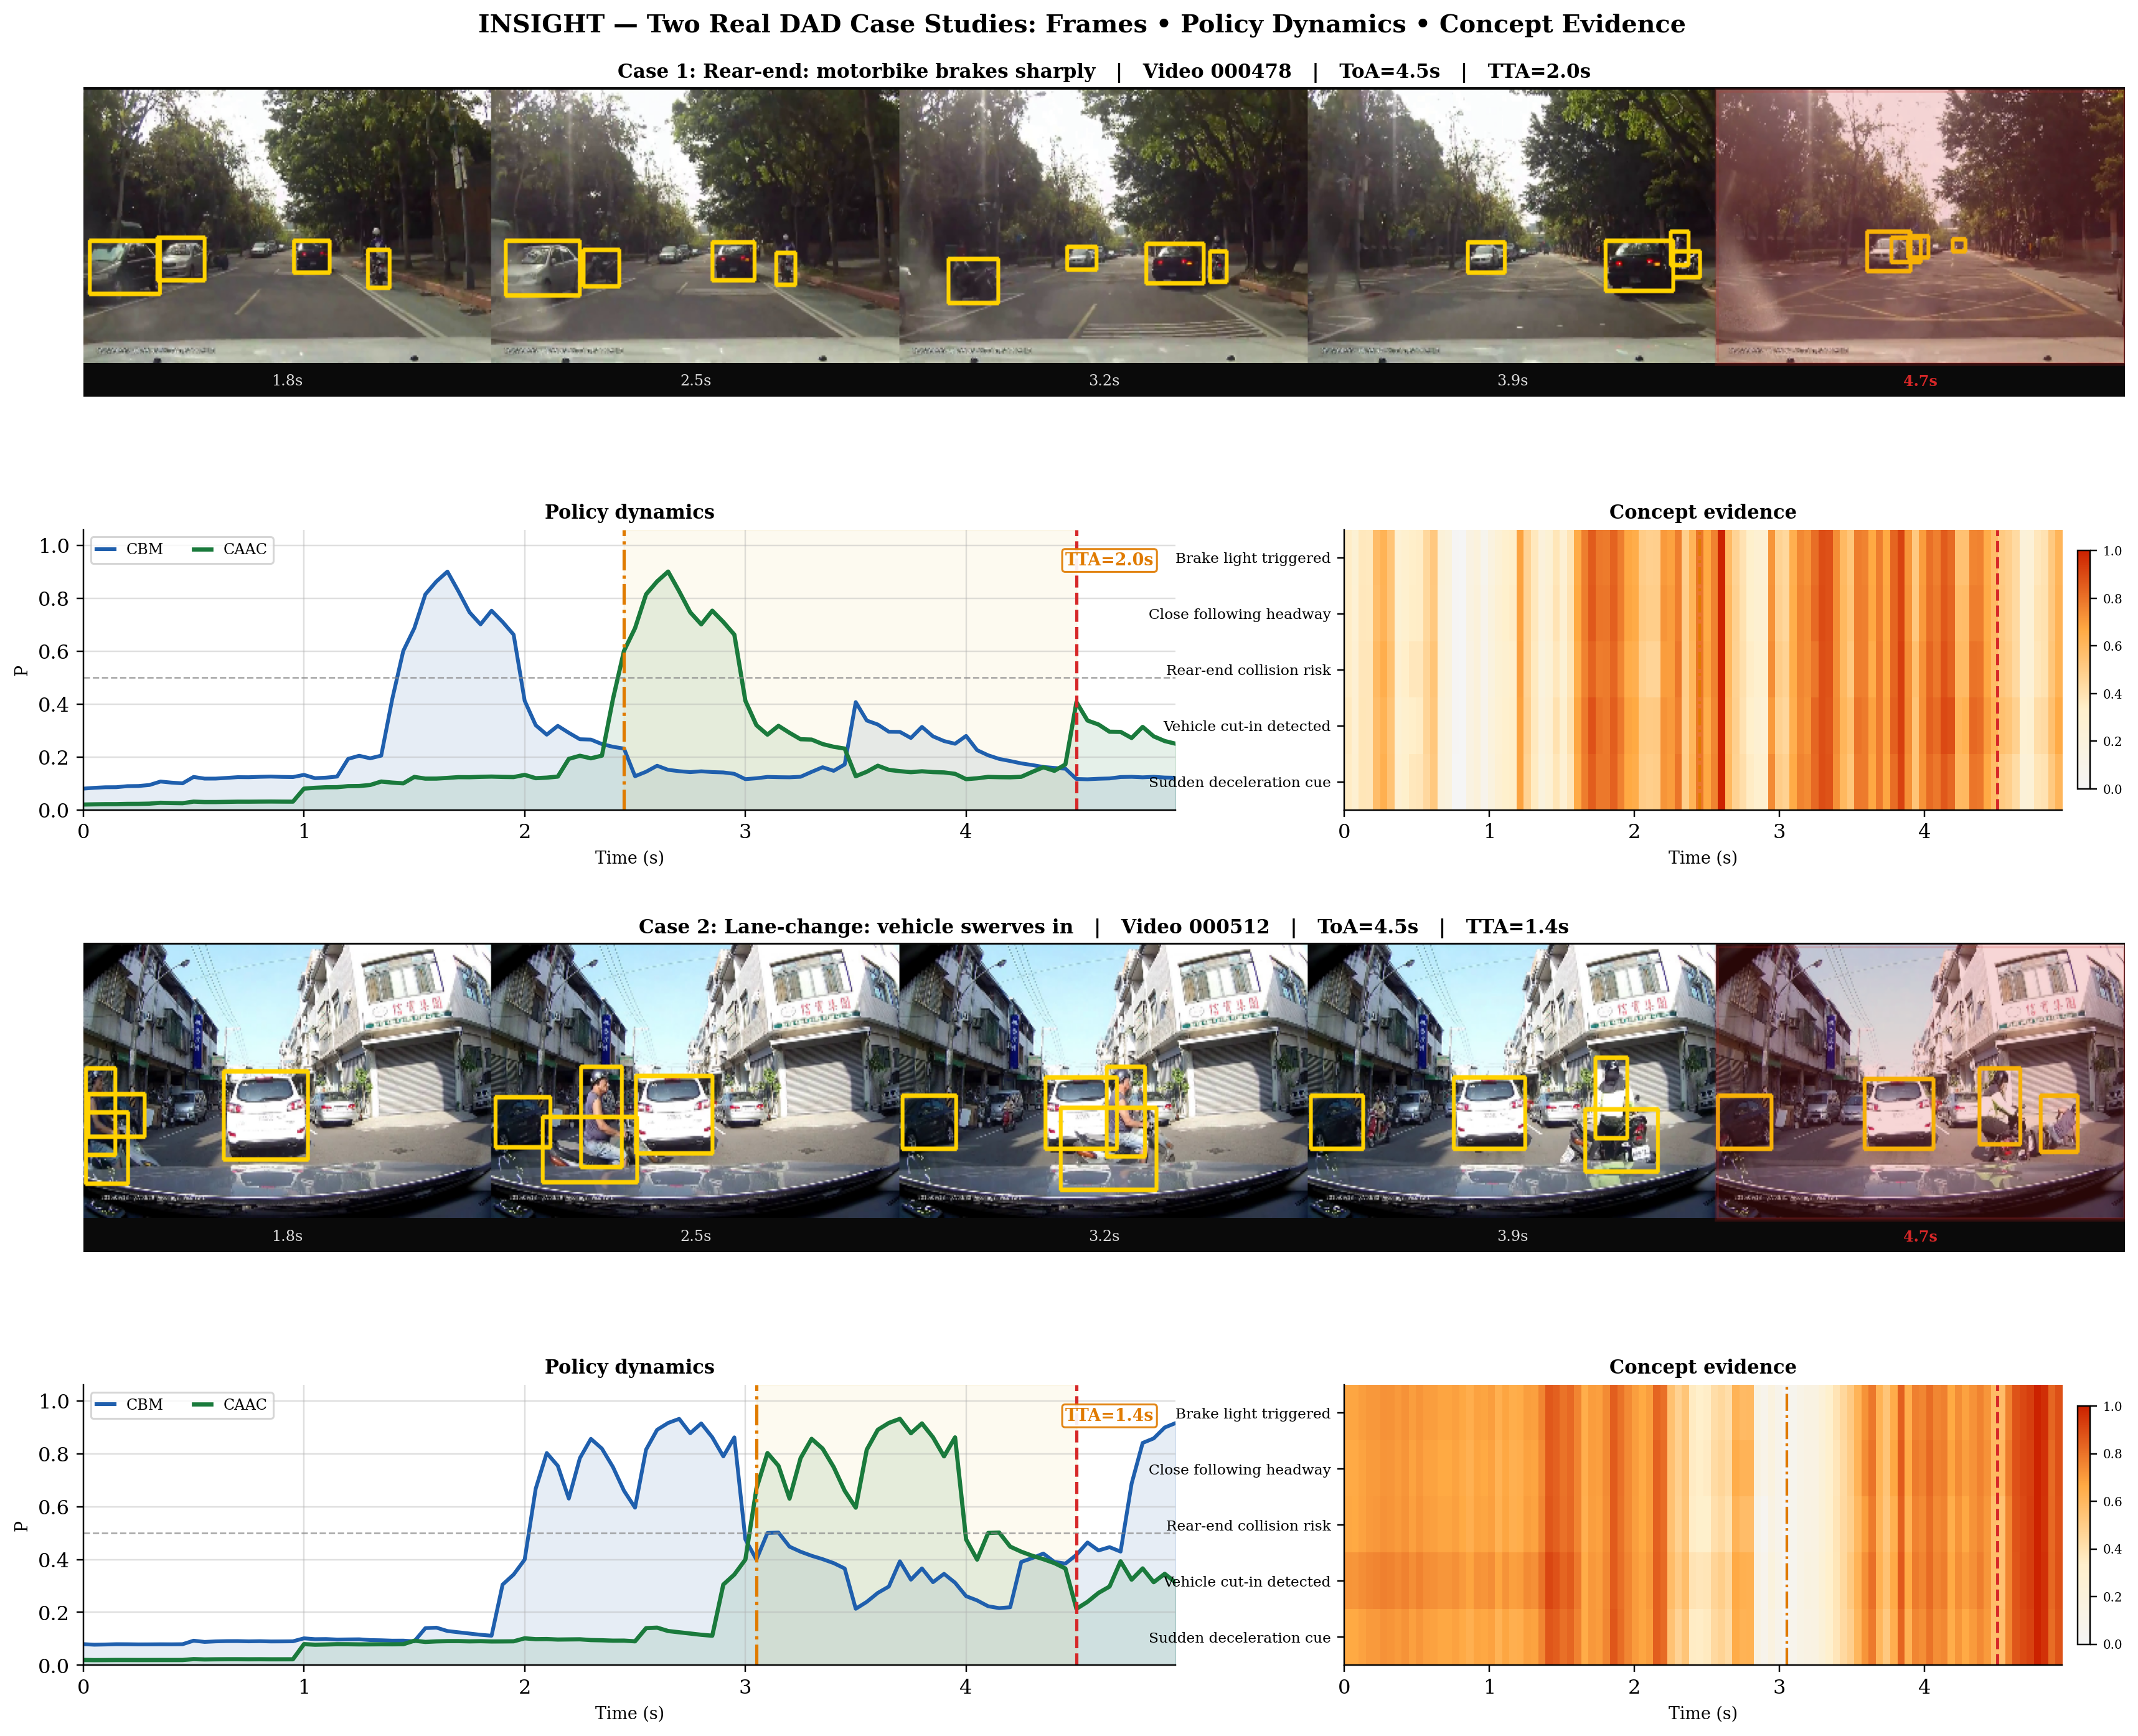
\includegraphics[width=0.98\textwidth]{../figures/insight_fig_appendix_v4_casebank_selected.pdf}
  \caption{\textbf{Selected v4 DAD cases ranked by prediction-branch behaviour.}
  Using the runnable v4 checkpoint, we extract a shortlist containing an
  earlier-warning case, near-threshold borderline cases, and a harder
  low-visibility example. Because the alert surrogate is nearly flat on this
  checkpoint line, the figure should be read as a prediction-level qualitative
  bank rather than as a policy-level alert benchmark.}
  \label{fig:appendix_v4_casebank_selected}
\end{figure*}

\paragraph{Case diversity.}
Across rear-end, lane-change, and intersection scenarios, the dominant
concepts change substantially, but the qualitative pattern stays similar: the
\cbm{} surfaces plausible risk factors first, and the downstream timing signal
responds as those factors rise. The appendix figures also show that visually
strong cases vary in difficulty, from clean agent separation to cluttered or
low-visibility scenes.

\paragraph{Policy-before-peak behaviour.}
In selected qualitative figures, the green \caac{} curve can cross its alert
threshold \emph{before} the blue raw accident-probability curve peaks. This is
consistent with the intended effect of the time-remaining reward: the timing
consumer can respond to a rising semantic trend rather than waiting for maximal
confidence. We present this as qualitative support for the design, not as a
standalone policy benchmark.

\paragraph{Frame--concept alignment.}
The strongest visual evidence occurs when a concrete scene change is mirrored
by a concept change: brake lights activate, headway shrinks, or a vehicle cuts
into the ego lane, and the corresponding concept rows intensify in the
heatmap. Not every high-scoring sample is equally legible, which is why case
selection matters for qualitative presentation.

\subsection{Failure Modes, Robustness Considerations, and Dataset-Specific Discussion}
\label{app:failure}

\paragraph{Low-visibility conditions.}
Night-time and poor-weather scenes remain challenging. In these settings, the
ROI features are weaker and concept activations become less reliable,
especially for fine-grained cues such as brake lights or subtle lane-boundary
signals. The resulting failure mode is usually concept under-activation rather
than an obviously incorrect timing policy.

\paragraph{Crowded scenes.}
When many agents are present simultaneously, the object-focused aggregation
must compress a large amount of interaction structure into a fixed hidden
state. This can dilute the representation of the single most critical risk
agent. A natural next step is a more explicit risk-agent selection mechanism
layered on top of the concept bottleneck.

\paragraph{Concept vocabulary coverage.}
Although 837 concepts provide broad coverage, rare corner cases still exist
where the needed concept is absent or too coarse. This is a limitation of any
finite concept vocabulary. Future work could investigate adaptive or
hierarchical concept sets that retain auditing benefits while improving
long-tail coverage.

\paragraph{Why A3D and DAD behave differently.}
The qualitative evidence suggests that the relative value of semantic
structuring is dataset-dependent. In A3D, many hazards develop progressively,
so early concept growth is especially useful for anticipation. DAD is harsher:
the margin between weak early signal and crash onset is smaller, and the scenes
are often more cluttered. This likely explains why DAD is both a harder
benchmark and a more sensitive test of concept reliability.

\paragraph{Robustness interpretation.}
The main robustness point is that the semantic interface remains useful across
multiple datasets and accident types even when controllability is not uniformly
strong across all checkpoints and scenes. The v4 appendix search therefore
serves as prediction-level qualitative support rather than as a policy-level
ranking result.
accident anticipation should be treated as a concept-conditioned sequential
decision problem, not merely as frame-wise classification with post-hoc
explanation.


\clearpage
\bibliography{insight}

\end{document}
